% 
%\iffalse meta-comment
%
% Copyright (C) 2017--2020 by Xiangdong Zeng <xdzeng96@gmail.com>
%
% This work may be distributed and/or modified under the
% conditions of the LaTeX Project Public License, either
% version 1.3c of this license or (at your option) any later
% version. The latest version of this license is in:
%
%   http://www.latex-project.org/lppl.txt
%
% and version 1.3 or later is part of all distributions of
% LaTeX version 2005/12/01 or later.
%
% This work has the LPPL maintenance status `maintained'.
%
% The Current Maintainer of this work is Xiangdong Zeng.
%
% \fi

%*********************************************************************
% fduthesis: 复旦大学论文模板
% 2020/08/30 v0.7e
%
% 重要提示:
%   1. 请确保使用 UTF-8 编码保存
%   2. 请使用 XeLaTeX 或 LuaLaTeX 编译
%   3. 请仔细阅读用户文档
%   4. 修改、使用、发布本文档请务必遵循 LaTeX Project Public License
%   5. 不需要的注释可以尽情删除
%*********************************************************************

\documentclass[type=master, oneside]{fduthesis}
% 模板选项:
%   type = doctor|master|bachelor  论文类型,默认为本科论文
%   oneside|twoside                论文的单双面模式,默认为 twoside
%   draft = true|false             是否开启草稿模式,默认关闭
% 带选项的用法示例:
%   \documentclass[oneside]{fduthesis}
%   \documentclass[twoside, draft=true]{fduthesis}
%   \documentclass[type=bachelor, twoside, draft=true]{fduthesis}

\fdusetup{
  % 参数设置
  % 允许采用两种方式设置选项:
  %   1. style/... = ...
  %   2. style = { ... = ... }
  % 注意事项:
  %   1. 不要出现空行
  %   2. “=” 两侧的空格会被忽略
  %   3. “/” 两侧的空格不会被忽略
  %   4. 请使用英文逗号 “,” 分隔选项
  %
  % style 类用于设置论文格式
  style = {
    % font = times,
    % 西文字体(包括数学字体)
    % 允许选项:
    %   font = garamond|libertinus|lm|palatino|times|times*|none
    %
    cjk-font = windows,
    % 中文字体
    % 允许选项:
    %   cjk-font = adobe|fandol|founder|mac|sinotype|sourcehan|windows|none
    %
    % 注意:
    %   1. 中文字体设置高度依赖于系统。各系统建议方案:
    %        windows:cjk-font = windows
    %        mac:    cjk-font = mac
    %        linux:  cjk-font = fandol(默认值)
    %   2. 除 fandol 和 sourcehan 外,其余字体均为商用字体,请注意版权问题
    %   3. 但 fandol 字体缺字比较严重,而 sourcehan 没有配备楷体和仿宋体
    %   4. 这里中西文字体设置均注释掉了,即使用默认设置:
    %        font     = times
    %        cjk-font = fandol
    %   5. 使用 font = none / cjk-font = none 关闭默认字体设置,需手动进行配置
    %
    font-size = -4,
    % 字号
    % 允许选项:
    %   font-size = -4|5
    %
    % fullwidth-stop = catcode,
    % 是否把全角实心句点 “.” 作为默认的句号形状
    % 允许选项:
    %   fullwidth-stop = catcode|mapping|false
    % 说明:
    %   catcode   显式的 “。” 会被替换为 “.”(e.g. 不包括用宏定义保存的 “。”)
    %   mapping   所有的 “。” 会被替换为 “.”(使用 LuaLaTeX 编译则无效)
    %   false     不进行替换
    %
    footnote-style = xits,
    % 脚注编号样式
    % 允许选项:
    %   footnote-style = plain|libertinus|libertinus*|libertinus-sans|
    %                    pifont|pifont*|pifont-sans|pifont-sans*|
    %                    xits|xits-sans|xits-sans*
    %
    hyperlink = none,
    % 超链接样式
    % 允许选项:
    %   hyperlink = border|color|none
    %
    % hyperlink-color = default,
    % 超链接颜色
    % 允许选项:
    %   hyperlink-color = default|classic|elegant|fantasy|material|
    %                     business|science|summer|autumn|graylevel|prl
    % 默认与西文字体保持一致
    %
    bib-backend = bibtex,
    % 参考文献支持方式
    % 允许选项:
    %   bib-backend = bibtex|biblatex
    %
    % bib-style = numerical,
    % 参考文献样式
    % 允许选项:
    %   bib-style = author-year|numerical|<其他样式>
    % 说明:
    %   author-year  著者—出版年制
    %   numerical    顺序编码制
    %   <其他样式>   使用其他 .bst(bibtex)或 .bbx(biblatex)格式文件
    %
    % cite-style = {},
    % 引用样式
    % 默认为空,即与参考文献样式保持一致
    % 仅适用于 biblatex;如要填写,需保证相应的 .cbx 格式文件能被调用
    %
    bib-resource = {refs.bib},
%    bib-resource = {fduthesis-template.bib},
    % 参考文献数据源
    % 可以是单个文件,也可以是用英文逗号 “,” 隔开的一组文件
    % 如果使用 biblatex,则必须明确给出 .bib 后缀名
    %
    % logo = {fudan-name.pdf},
    % 封面中的校名图片
    % 模版已自带,通常不需要额外配置
    %
    % logo-size = {0.5\textwidth},      % 只设置宽度
    % logo-size = {{}, 3cm},            % 只设置高度
    % logo-size = {8cm, 3cm},           % 设置宽度和高度
    % 设置校名图片的大小
    % 通常不需要调整
    %
    % auto-make-cover = true
    % 是否自动生成论文封面(封一)、指导小组成员名单(封二)和声明页(封三)
    % 除非特殊需要(e.g. 不要封面),否则不建议设为 false
  },
  %
  % info 类用于录入论文信息
  info = {
    title = {针对精密直线运动平台的滑模控制方法研究}, 
    % 中文标题
    % 长标题建议使用 “\\” 命令手动换行(不是指在源文件里输入回车符,当然
    % 源文件里适当的换行可以有助于代码清晰):
    %   title = {最高人民法院、最高人民检察院关于适用\\
    %            犯罪嫌疑人、被告人逃匿、死亡案件违法所得\\
    %            没收程序若干问题的规定},
    %
    title* = {Research of Sliding Mode Control Method for Precision Linear Motion Stages},
    % 英文标题
    %
%    author = {王攀},
     author = {XXX},
    % 作者姓名
    %
    % author* = {Your name},
    % 作者姓名(英文 / 拼音)
    % 目前不需要填写
    %
%    supervisor = {杨晓峰\quad 教授},
    supervisor = {XXX},
    % 导师
    % 姓名与职称之间可以用 \quad 打印一个空格
    %
    major = {微电子学与固体电子学},
    % 专业
    %
    degree = academic,
    % 学位类型
    % 允许选项:
    %   degree = academic|professional
    % 说明:
    %   academic      学术学位
    %   professional  专业学位
    %
    department = {工程与应用技术研究院},
    % 院系
    %
%    student-id = {18210860016},
    student-id = {18210860016},
    % 作者学号
    %
    date = {2021 年 3 月 31 日},
    % 日期
    % 注释掉表示使用编译日期
    %
    % secret-level = ii,
    % 密级
    % 允许选项:
    %   secret-level = none|i|ii|iii
    % 说明:
    %   none  不显示密级与保密年限
    %   i     秘密
    %   ii    机密
    %   iii   绝密
    %
    % secret-year = {五年},
    % 保密年限
    % secret-level = none 时该选项无效
    %
%    instructors = {
%      {杨晓峰\quad\,\,\,\,\,\, 教\quad 授\quad \quad},
%      {丁晨阳     \quad 青年研究员},
%      {殳\quad 峰 \quad 青年研究员},
%      {张志平     \quad 青年研究员}
%    },
    % instructors=none,
    % 指导小组成员
    % 使用英文逗号 “,” 分隔
    % 如有需要,可以用 \quad 手工对齐
    %
    keywords = {精密直线运动平台, 系统辨识, 递推最小二乘, 神经网络, 滑模控制},
    % 中文关键字
    % 使用英文逗号 “,” 分隔
    %
    keywords* = {precision linear motion stage, system identification, recursive least squares, neural network, sliding mode control},
    % 英文关键字
    % 使用英文逗号 “,” 分隔
    %
    clc = {TP273+.2}
    % 中图分类号
  }
}

% 需要的宏包可以自行调用
\usepackage{physics}
%\input fduthesis-test-toolkit
\usepackage{float}
\usepackage{subfig}
%\usepackage{subfigure}
\usepackage{cases}
%%
\usepackage{multirow}
\usepackage{booktabs}
\usepackage{threeparttable}
\usepackage{textcomp}
\usepackage{siunitx}  %可以输入摄氏度
\usepackage{subfig}
\usepackage{bm}
%\usepackage{mathastext}
%%

%%
\makeatletter  
\newif\if@restonecol  
\makeatother  
\let\algorithm\relax  
\let\endalgorithm\relax  
\usepackage[linesnumbered,ruled,vlined]{algorithm2e}
\usepackage{algpseudocode}
\usepackage{lscape}
\usepackage{url}
\renewcommand{\algorithmicrequire}{\textbf{Input:}} 
\renewcommand{\algorithmicensure}{\textbf{Output:}} % Use Output in the format of Algorithm%
%%
\usepackage{verbatim}
% 需要的命令可以自行定义
\newcommand{\hilbertH}{\symcal{H}}
\newcommand{\ee}{\symrm{e}}
\newcommand{\ii}{\symrm{i}}

\makeatletter
\fancyhead[L]{}
\fancyhead[R]{}
\fancyhead[C]{\fdu@kai\zihao{-3}复~旦~大~学~硕~士~学~位~论~文}
\let\ps@plain\ps@fancy
\patchcmd{\l@chapter}
  {\hfil}
  {\leaders\hbox{\normalfont$\m@th\mkern \@dotsep mu\hbox{.}\mkern \@dotsep mu$}\hfill}
  {}{}
\makeatother

\begin{document}

\frontmatter

% 目录
\tableofcontents
%% 插图目录
%\listoffigures
%% 表格目录
%% \listoftables

\begin{abstract}
芯片尺寸的不断缩小对扫描投影光刻机提出了严峻的挑战,其中,完成大量直线扫描运动的工件台及其控制是重要瓶颈之一。直线电机作为核心的执行机构,一直是研究的焦点和热点。但是,直线电机自身所含有的模型参数摄动、定位力、电磁非线性以及外部扰动等因素严重影响其位置跟踪性能,因此,如何克服上述影响因素成为实现精密直线运动平台高性能控制的关键。

本文以光刻机工件台为研究背景,针对上述核心问题,从基于直线电机的精密直线运动平台系统建模和滑模控制算法方面开展研究。主要研究内容和结论如下:

1) 建立了一种新的基于神经网络的扰动模型。该模型充分考虑了精密直线运动平台的各种非线性扰动,并将其分为时变和时不变两部分,并结合在线自适应补偿方法实现对各种非线性扰动的补偿。此外,对系统进行了初步的参数辨识,获得了系统的等效质量、等效阻尼和定位力最大空间周期,为后文控制器的设计奠定了基础。

2) 提出了一种改进型递推最小二乘积分滑模控制方法(Improved Recursive Least Square Integral Sliding Mode Control, IRLSISMC)。该方法在传统递推最小二乘积分滑模控制(Traditional Recursive Least Square Integral Sliding Mode Control, TRLSISMC)的基础上,将精密直线运动平台定位力的主要成分引入到递推最小二乘算法的回归向量中,实时地进行逆模型前馈控制和定位力补偿。与此同时,积分滑模反馈控制部分保证了位置跟踪误差渐近收敛到0,并通过李雅普诺夫理论证明了系统稳定性。


3) 提出了一种多核神经网络滑模控制方法(Multi-Kernel Neural Network Sliding Mode Control, MNNSMC)。该方法由多核神经网络(Multi-Kernel Neural Network, MNN)和带有动态边界层的滑模控制两部分组成。前者考虑了所研究的精密直线运动平台的动力学特性,将定位力与摩擦力的经典模型考虑进神经网络核函数的设计中,不仅保留了典型的高斯径向基函数,还引入了三角核函数和sigmoid核函数,分别在线拟合并补偿定位力与摩擦力引起的扰动。后者采用的动态边界层可以根据系统的速度信息实时地进行边界层厚度的调整,有助于系统状态轨迹收敛到滑模面,同时构建了李雅普诺夫函数,证明了MNNSMC的渐近稳定性。

4) 设计了三组不同设置的位置跟踪实验,验证了所提方法在精密直线运动平台上的高性能控制效果。与传统方法相比,IRLSISMC方法和MNNSMC方法能够有效地提升系统的位置跟踪精度和扰动抑制能力,并对模型参数摄动有一定的鲁棒性。
\pagenumbering{Roman}
\end{abstract}



\begin{abstract*}
 The continuous shrinking of chip size poses severe challenges to the scanning projection lithography machine. Among them, the wafer stage that completes a large number of linear scanning motions is one of the important bottlenecks. As the core actuator, the linear motor has always been the focus and hotspot of research. However, the linear motor itself contains model parameter variations, positioning force, electromagnetic nonlinearity, and external disturbance that seriously affect its position tracking performance. Therefore, how to overcome the above influencing factors has become the key to achieving high-performance control of precision linear motion stages.
 
 This thesis takes the lithography machine's wafer stage as the research background, aiming at the aforementioned core problems, and researches from the aspects of the precision linear motion stage model based on the linear motor and the sliding mode control method. The specific research contents and conclusions are as follows:
 
 1) Developed a new disturbance model based on neural network. The model fully considers the various nonlinear disturbances of the precision linear motion stage, and divides them into two parts, time-varying and time-invariant, and combines the adaptive control method to realize the compensation of various nonlinear disturbances online. In addition, preliminary parameter identification of the system was carried out, and the equivalent mass, equivalent damping and maximum space period of the positioning force of the system were obtained, which laid the foundation for the design of the controller later.
 
 2) Proposed an improved recursive least square integral sliding mode control (IRLSISMC) method. Based on the traditional recursive least square integral sliding mode control (TRLSISMC), this method introduces the main component of the positioning force of the precision linear motion stage into the regression vector of the recursive least squares algorithm to realize inverse-model-based feedforward control and positioning force compensation. At the same time, the integral sliding mode feedback control ensures that the position tracking error asymptotically converges to zero, and the system stability is proved by the Lyapunov theorem.
 
 
 3) Proposed a multi-kernel neural network sliding mode control (MNNSMC) method. This strategy consists of two parts: multi-kernel neural network (MNN) and sliding mode control with dynamic boundary layer. The former considers the dynamic characteristics of the studied precision linear motion stage, and introduced the classic models of positioning force and friction into the design of kernel functions, not only retaining the typical Gaussian radial basis function, but also introducing triangular functions and sigmoid function to fit and compensate for the disturbances caused by positioning force and friction, respectively. The latter can adjust the thickness of the boundary layer in real time according to the velocity of the mover, which helps the system state trajectory converge to the sliding manifold asymptotically. At the same time, the Lyapunov theorem is constructed to prove the asymptotic stability of MNNSMC. 
 
 4) Designed three different position tracking experiments settings to verify the high-performance control effect of proposed methods on a precision linear motion stage. Compared with traditional methods, the IRLSISMC method and MNNSMC strategy can effectively improve the system's position tracking accuracy and disturbance suppression ability, and have certain robustness to the model parameter variations.
\end{abstract*}

% 符号表
% 语法与 LaTeX 表格一致:列用 & 区分,行用 \\ 区分
% 如需修改格式,可以使用可选参数:
%   \begin{notation}[ll]
%     $x$ & 坐标 \\
%     $p$ & 动量
%   \end{notation}
% 可选参数与 LaTeX 标准表格的列格式说明语法一致
% 这里的 “ll” 表示两列均为自动宽度,并且左对齐
%\begin{notation}[lp{20em}]
%	$\sin$      &  正弦 \\
%	HPC         &  高性能计算 (High Performance Computing) \\
%	cluster     &  集群 \\
%	Itanium     &  安腾 \\
%	SMP         &  对称多处理 \\
%	API         &  应用程序编程接口 \\
%	PI          &  聚酰亚胺 \\
%	MPI         &  聚酰亚胺模型化合物,N-苯基邻苯酰亚胺 \\
%	PBI         &  聚苯并咪唑 \\
%	MPBI        &  聚苯并咪唑模型化合物,N-苯基苯并咪唑 \\
%	PY          &  聚吡咙 \\
%	PMDA-BDA    &  均苯四酸二酐与联苯四胺合成的聚吡咙薄膜 \\
%	$\Delta G$  &  活化自由能 (Activation Free Energy) \\
%	$\chi$      &  传输系数 (Transmission Coefficient) \\
%	$E$         &  能量 \\
%	$m$         &  质量 \\
%	$c$         &  光速 \\
%	$P$         &  概率 \\
%	$T$         &  时间 \\
%	$v$         &  速度
%\end{notation}

\mainmatter

\chapter{绪论}
\section{课题来源}
本课题来自国家科技重大专项“极大规模集成电路制造装备及成套工艺”(02专项)28nm节点浸没式光刻机产品研发项目子课题七“浸没光刻机亚纳米精度运动控制技术研究”(课题编号2017ZX02101007)。
\section{研究背景与意义}
扫描投影光刻机是半导体制造领域地位最为重要、技术难度最大、复杂程度最高的设备,也是目前芯片特征尺寸逐渐缩小,功能不断强大的有力保障。随着摩尔定律和后摩尔时代的发展,芯片的集成度将仍保持指数级增长,3$\sim$5纳米工艺节点呼之欲出。这种必然的趋势对整个集成电路产业链,包括设计、制造、封装和测试均提出了更高的要求,尤其是芯片制造领域,意味着未来必然迎来各种极大规模集成电路制造设备与工艺的升级换代。

集成电路的快速发展得益于光刻工艺的不断进步。在光刻工艺中,光刻机是决定性的设备,其必须同时满足芯片制造的关键尺寸、套刻精度和产率三大核心要求。如图\ref{光刻原理图1}所示,光刻机主要由光源及其控制系统、运动台及其控制系统以及环境控制系统等构成。整个光刻控制系统可以说是该设备的“大脑”,必须时刻维持高速、精准的控制,其作用主要是对硅片以及印有电路图形的掩模版进行超高精度、超高速度的操作,同时实现多自由度的空间相对运动,保证设计好的电路图形可以在亚纳米精度准确无误地曝光到硅片上,完成图形的转移。从实际需求考虑,光刻机控制技术的挑战主要集中在三个方面\cite{butler2011position}:1)小尺寸。现代集成电路芯片的特征尺寸逐渐缩小,已达到纳米级甚至亚纳米级,要保证电路图形精准地刻画在晶圆上,扫描曝光过程中允许的位置误差只有几纳米甚至不到1纳米,仅为特征尺寸的一小部分;2)高产率。光刻机用于大规模批量生产线,对产率的要求很高,通常每小时的产量为175片以上;3)高鲁棒性和可靠性。实际工业生产线上,保证机器持续稳定地工作是必然的追求,这与测量系统、环境调节和控制策略都有很大关系。

从运动台及其控制角度来看,曝光成像过程要在高速运动中完成,其扫描和定位精度直接影响曝光成像质量,包括成像精度和套刻精度,因此对光刻机运动系统的扫描和定位精度要求达到纳米级精度甚至亚纳米级精度。另一方面,高产率的需求要求运动系统具有高速高加速的特性,而高速高加速引起的振动会导致精度恶化、整定时间变长,从而导致产率下降。可以看出,高速度、高加速度、高精度以及高产率之间是相互矛盾的,需要采用额外的控制措施使得相互制约的性能指标都达到一个较为理想的值,这是一个非常具有挑战的工作。

\begin{figure}[!t]
	\centering
	\includegraphics[width=12cm]{figures/光刻原理图2}
	\caption{ASML扫描投影光刻机}
	\label{光刻原理图1}
\end{figure}
\begin{comment}
在扫描光刻控制系统领域,大部分还是使用闭环PID反馈控制器,PID 控制器的优点是明显的:简单好用,P,I,D 各项物理意义明确,稍有研究即可对其进行参数调试。基于PID解耦控制技术的传统工件台运动控制方法虽然已经取得了较好的效果[2-4],而且现在很多中低端光刻控制系统中仍然在使用传统PID控制方法,但是传统PID控制方法存在的一些问题限制了扫描光刻系统性能的进一步提升。首先,PID方法仅能解决单输入-单输出(SISO)控制问题。虽然现在运用解耦控制技术,可以将多输入-多输出(MIMO)通过解耦转换为单输入-单输出(SISO)控制问题。但实际效果很大程度上取决于解耦过程以及系统各变量之间的复杂关系,另外需要考虑系统各变量自身的稳定性,这些要求在工业环境中极为苛刻,很难保证完全解耦且系统各变量自身不随环境变化而变化。其次,传统PID方法缺乏对非线性因素的考虑,而扫描光刻系统的工件台控制存在非线性因素的影响,此外由于负载的变化、外界的扰动以及设备自身的磨损等因素引起的模型不确定性和一些未建摸特性都会影响传统PID控制系统的鲁棒性和稳定性。最后,PID 参数本身整定困难,而且一组参数一般只适用于一种工况,对时变的,动态的,非线性的,复杂的系统适应性差,而且在系统快速性和稳定性上难以同时兼顾。在这种情况下,针对原来系统模型设计的PID控制器不再合理,甚至失效,以至无法达到理想的控制效果。因此,对PID控制器的参数整定的研究具有重要的意义。
\end{comment}


光刻机运动台包括工件台和掩模台,其高速度和高加速度基本上都是由精密直线运动平台作为执行机构产生\cite{butler2011position},因此,要平衡高速度、高加速度、高精度以及高产率等性能要求,对精密直线运动平台进行高性能运动控制是重要突破点之一。精密直线运动平台经历了机械导轨、气浮导轨以及磁浮导轨的发展,但是不变的是执行机构大都是基于永磁同步直线电机(Permanent Magnet Synchronous Linear Motors, PMLSMs)或其变种,因此本文将基于PMLSMs的精密直线运动平台作为研究对象。如图\ref{直线电机结构}所示,相比于传统基于旋转电机的直线运动平台,PMLSMs摆脱了中间传动机制的限制,因而更适用于高速、高加速定位系统,然而,由于省略了中间传动机构,定位力、线缆力、纹波扰动以及模型参数摄动和外部扰动等不确定性因素将直接影响PMLSMs的位置跟踪性能\cite{wang2015detent}。因此,如何提高系统的扰动抑制能力成为实现PMLSMs高性能控制的关键\cite{yang2018investigation}。

PMLSMs的端部力和齿槽力合称为定位力,与电机的磁体结构有关,是一种不依赖于时间的扰动,只与PMLSMs动子运动的位置相关。线缆力也是一种位置依赖的扰动,其与位置的关系也呈现出典型的非线性特性\cite{yang2018integrated}。已经有很多经典模型被提出\cite{tan2002robust,chen2009modeling,wassink2005lpv},通过建模的方式能够在一定程度上消除定位力和线缆力对于PMLSMs位置跟踪性能的影响,但要进一步提高控制性能,还需要对定位力和线缆力的未建模部分以及纹波扰动、模型参数摄动、未知的外部扰动等时变的非线性扰动进行一定的补偿。
非线性扰动已经是影响工件台精度的主要原因之一。由于含有具有开关特性的鲁棒项,滑模控制能够有效地抑制非线性扰动\cite{heertjes2014self,li2016state}。自提出以来,滑模变结构控制已经拥有了非常成熟的一套理论体系\cite{young1999control},而且滑模控制方法简单易用,能够很自然地与自适应控制\cite{huang2008adaptive}、模糊控制\cite{tong2003fuzzy}以及神经网络控制\cite{qi2013adaptive}相结合,如今在精密运动控制领域也得到了广泛的应用。神经网络在处理非线性问题的时候,由于其对于非线性函数有着良好的拟合能力,且不需要具体的模型信息,因此对于补偿未知的时变扰动非常有优势。从实际应用的角度考虑,如果能够充分发挥滑模控制以及神经网络在非线性控制方面的优势,将非常有利于解决扫描光刻系统工件台控制面临的非线性影响因素带来的问题。
\begin{figure}[!t]
	\centering
	\includegraphics[width=12cm]{figures/直线电机结构图.pdf}
	\caption{永磁同步直线电机结构}
	\label{直线电机结构}
\end{figure}



本文通过对有铁芯PMLSMs动力学与扰动形式进行分析与建模,并结合递推最小二乘算法和神经网络的特性,对滑模变结构控制中的应用进行深入研究,旨在探索基于滑模控制的高性能运动控制方法来提高精密直线运动平台的位置跟踪性能和扰动抑制能力,以便其能够更广泛地应用于精密运动控制领域。
\section{精密直线运动平台控制方法研究现状及分析}
精密直线运动平台作为精密运动系统中的核心运动部件,广泛应用于集成电路制造、超精密伺服加工、纳米精度测量以及生物信息检测等领域\cite{董泽光2014精密气浮运动平台的建模}。在实际工程应用需求中,高速、高加速、高精度以及高稳定性是精密直线运动平台控制系统设计的主要目标。面临的控制方面的挑战主要来自于机械系统本身的谐振、定位力、测量噪声、参数摄动和电磁非线性以及外部非线性扰动等。在这些影响因素存在的情况下跟踪精度要达到纳米级,同时满足高产率的要求是一个极具挑战的工作。为了实现这些目标,国内外很多研究机构以及企业研发机构已经提出很多控制方法,这里对主要的几种控制方法做简要介绍。
\subsection{比例-积分-微分控制}
比例-积分-微分(Proportional-Integral-Derivative, PID)控制凭借其简单易用、物理意义明显等优势已经统治工程应用领域数十年,尤其是对于能够精确建模的应用对象,PID控制器能够实现良好的控制性能。但是随着技术的不断进步,对于精度和速度的极致追求使得传统的PID反馈控制方法面临了很多挑战。因此,现在的精密运动系统中常以改进的PID控制器作为反馈控制部分。Heertjes等人\cite{2009Performance}提出了一种N-PID,基于非线性滤波器,对经典PID控制方法进行了改进,从而提高光刻机工件台控制系统的位置跟踪性,并构建了李雅普诺夫函数,证明了其稳定性。Shin等人\cite{2011Anti}针对控制器输出饱和问题,提出了一种预测饱和稳态值的方法,让系统控制输出退出饱和时,将预测的稳态值引入积分环节并作为积分环节的初值,这样控制器的输出就能够很大程度上避免因饱和问题带来的超调大和整定时间长的问题,实验结果表明了所提方法在PID控制器存在输出饱和现象时拥有较好的控制性能。王学伦等人\cite{wang2011design}介绍了一种复合模糊免疫PID,用于PMLSMs的速度环,有效地提高了速度环的响应速度,通过自适应调节减小了速度环的误差。2014年,王辉和张段芹等\cite{王辉2014新型智能}提出了一种反向传播神经网络PID控制策略,网络的输出为PID参数,通过自适应的方法进行实时更新,有效地改善了基于永磁同步直线电机的调速系统的性能。2018年,一种基于扩张状态观测器的PID控制器被提出\cite{王文深2018基于},提高了气动机械手系统的定位精度和响应速度。2020年,一种基于粒子群优化的PID控制算法应用于微电子封装领域\cite{2020A},通过粒子群优化算法整定PID参数,改善了系统的控制指标。

PID控制器在运动控制领域的应用虽然仍旧非常普遍,但是随着跟踪精度要求越来越高,在超精密运动控制领域,单纯使用PID反馈控制器,实现高速、高精度控制有较大的挑战。因此,前馈控制与反馈控制相结合的方式引起了很多学者和工程师的关注。
\subsection{迭代学习控制}
迭代学习控制(Iterative Learning Control, ILC)是一种应用于重复参考轨迹的前馈控制方法,早期的期刊文献是1978年发表在日文期刊\cite{uchiyama1978formation},最初主要用于机械臂的重复轨迹控制中。ILC真正在学术界流行是1984年一系列文章\cite{1998Adaptive,kawamura1984iterative}发表之后,人们才认识到了ILC学习算法的重要价值。ILC作为一种前馈控制方式,不需要精确的数学模型,通过误差的迭代计算,即可学习到用于补偿扰动的补偿表,从而极大地提高系统的跟踪精度。Mishra等人\cite{mishra2010optimization}提出了一种基于优化约束的ILC设计方法,在执行器饱和约束的情况下采用跟踪误差的$L_2$范数作为评价指标,利用凸优化的思想设计得到ILC控制方法,提高了光刻机工件台位置跟踪性能,文章的主要贡献也是将数值优化的方法应用到了ILC的设计之中。Abidi等人\cite{abidi2010iterative}提出了一种基于时频域的ILC设计和分析的框架,比较了经典的P型、D型、D$^2$型和滤波器型的ILC的时频域特性,给出了采样时间与ILC收敛率之间的关系,对于ILC的设计提供了一种理论指引,最后还在压电平台上对于提出的设计框架进行了验证,仿真和实验结果都进一步表明所提设计准则的有效性。2007年,针对光刻机掩模台的一些非线性问题,Heertjes等人\cite{heertjes2007nonlinear}提出了一种非线性ILC,非线性主要体现在学习增益的设计中,在收敛速率和噪声抑制的平衡方面有了很大的改善。张等人\cite{zhang2018data}提出了一种局部动态线性化的方法被应用于针对非线性系统的自适应迭代学习控制系统设计中,整个系统的设计不依赖于模型信息,完全依赖于系统输入输出的数据,最后通过仿真验证了这种线性化的技术有益于数据驱动的ILC在非线性系统中的应用。Hao等人\cite{hao2020extended}针对工业批处理过程中的时变的不确定和外部扰动问题,提出了一种时域和迭代域相结合的ILC,这种ILC方法采用了双环结构,内环用基于扩张状态观测的反馈控制结构保证位置跟踪时间上的鲁棒性,外环采用P型ILC保证批处理过程的收敛性,还基于线性矩阵不等式保证了整个控制系统的输出是有界的。ILC在重复扰动占主导地位的控制系统中能够保证很好的控制性能,但是当系统中的非重复扰动占主导时,往往ILC控制性能会变差\cite{mishra2007precision}。为了解决基于采样数据的迭代学习控制在非重复扰动存在情况下的收敛性问题,池荣虎等人\cite{chi2020convergence}提出了一种新的分析方法,结合数学归纳法与收缩映射原理证明了系统变量的有界收敛性,并证明了当迭代变化的不确定性消失的情况下,系统跟踪误差能够收敛到一个较小的边界,这些结构都能够放松ILC限制性的重复条件。

但是在实际工业应用环境中,系统模型参数可能会出现摄动现象,即模型参数会随着时间有微小的变化,这种情况下,ILC作为一种典型的前馈控制方法,对于模型参数的变化非常敏感,进而会影响系统的跟踪精度。针对这种模型参数摄动等需要在线调节和控制的问题,人们对自适应控制寄予了更多期待。
\subsection{自适应控制}
自适应控制主要用来应对系统不确定性随时间或空间变化的情况,控制器能够根据系统状态的变化实时地进行调整以提高系统的跟踪性能和扰动抑制能力。2012年,Butler\cite{butler2012adaptive}针对光刻机工件台中位置依赖的扰动,提出了一种自适应前馈的方式,通过在线调整系统前馈控制器参数提高了系统的位置跟踪精度并缩短了系统曝光前的整定时间,该文通过很多的实际工程问题验证了高阶前馈控制器能够比仅采用加速度前馈更有效地减小位置跟踪的误差峰值。针对PMLSMs系统存在的周期性的扰动,一种新型的自适应扰动补偿策略被提出\cite{cho2014high},主要用来减小重复性的扰动,这一新型的自适应扰动观测器不依赖于扰动的模型,在每个时间周期内通过更新周期的自适应律进一步地削弱扰动带来的影响。张等人\cite{zhang2019force}将模型参考自适应(Model Reference Adaptive Control, MRAC)和周期自适应学习控制(Periodic Adaptive Learning Control, PALC)相结合,提出了一种新的补偿方法(MRAC-PALC),这种新的补偿方案采用了“分段函数”的思想,在首次迭代中使用MARC获取初始信息,在之后的迭代过程中,使用PALC从上次迭代的信息中学习并更新控制器参数来补偿扰动,文章也通过Lyapunov理论证明了所提方法的稳定性,所提方法在PMLSMs实验平台进行了验证,证明了其有效性。王树波等人\cite{wang2020parameter}提出了一种新的参数估计方法,用来估计含有摩擦力的非线性系统中的未知参数,与经典的自适应律相比,该方法引入了额外的滤波器在线提取估计误差来获得新的更新律,并将这种自适应的方法与鲁棒积分反馈机制相结合补偿有界的扰动,系统性能明显改善。2020年,付等人\cite{fu2020frequency}基于数据驱动的思想,提出了一种基于频域辨识的自适应ILC方法,该方法不需要系统模型的结构和参数,能够有效地避免模型参数适配带来的性能恶化问题,给出了详细的理论证明并在直线运动平台上进行了实验验证。

虽然自适应控制能够较好地改善系统模型参数摄动等问题,但是当外界非线性扰动形式较为复杂时,自适应控制的收敛速度会受到很大影响,而非线性扰动在超精密运动控制领域越来越不容忽视,因此,能够有效抑制非线性扰动的控制方法备受瞩目。
\begin{comment}
\subsection{精密直线运动平台PID控制器参数整定研究现状}
由于PID控制器在工业中应用极为广泛,但是其参数的调节比较依赖于经验,尤其是面对较为复杂的控制对象,参数调节在整个控制系统搭建中往往是最耗时耗力的。近年来,PID控制器参数的整定问题受到了越来越多的学者重视,相关的理论也在不断完善。

Ziegler和Nichols\cite{ziegler1942optimum}于1942年基于一阶惯性环节加纯延迟的被控对象,成功展示了PID控制器参数整定的Z-N法,对于一般被控对象,可以用一阶惯性环节加纯延时的模型近似拟合其阶跃响应曲线。由于该方法的简单易用,很快便在工业界得到了应用。同年,Ziegler又提出了临界振荡法来调整PID控制器参数\cite{黄友锐2010pid},在已知系统临界比例增益和振荡周期的情况下,根据经验公式即可得到PID控制参数。庄敏霞等人\cite{张建国2004pid}介绍了几种PID参数整定的优化准则,基于优化的思想进行控制器参数的整定,此方法理论上可行,实际应用过程中,符合工程实际指标的优化准则往往较难确定,因此该方法的工程应用并没有特别广泛\cite{黄友锐2010pid}。曾振平等人\cite{曾振平2004基于新的误差积分准则的}提出了一种改进的广义的误差积分准则(RGISE),用响应特征时间平衡广义平方误差积分准则中误差以及误差的导数之间的数量级,获得了较大的幅值稳定裕度,系统的响应曲线也得到了改善。曾庆山等人\cite{曾庆山2004分数阶}提出了一种分数阶PID参数整定方法,将传统PID控制器参数整定方法推广到分数阶,该方法不仅可以用于分数阶滑模,仍然可以用于其他整数阶实验系统,设计方法有较为普遍的适用性。张立群等人\cite{张立群2005h}基于线性时不变(LTI)系统提出了一种基于$H_\infty$优化的PID控制器参数整定方法,该优化指标采用混合灵敏度函数作为目标函数,获得了有较强鲁棒性的PID控制器。随着启发式优化算法的快速发展,很多学者将智能优化算法应用到PID控制器参数整定问题中。2006年,李丽香等人\cite{李丽香2006基于混沌蚂蚁群算法的}提出了一种基于混沌蚁群算法的参数整定方法,属于群智能理论中的一种,该方法以误差的积分为性能指标,以增益和相位裕度为约束,对PID控制器参数进行优化选择,获得了性能较优的PID控制器。同年,张怀相等人\cite{张怀相2006基于迭代学习控制的}将迭代学习控制的思想应用到PID控制器参数的整定问题中,提出了一种基于PD型迭代学习控制的PID控制器参数整定方法,通过仿真和实验验证了基于此方法获得的PID控制器能够提升系统的动态性能和鲁棒性。马建伟博士\cite{马建伟0多指标满意}在其博士论文中提出了一种多目标满意PID控制方法,该方法基于状态空间分析方法,建立了多目标的$H_\infty$优化指标,通过Lyapunov稳定性理论得到了一整套计算PID控制器参数的方法,提高了PID控制器的鲁棒性。李银伢等人\cite{李银伢2007基于参数空间图解法的多目标满意}于2007年又提出了基于参数空间图解法的多指标满意PID控制器,该方法应用边界穿越定理,基于区域极点指标和$H_\infty$指标得到了计算参数解集的方法,并通过一个算例证明了所提方法的有效性。吕建婷等人\cite{吕建婷2008卫星姿态调节的滑模}针对卫星姿态控制问题提出了一种滑模PID控制器,基于Lyapunov稳定性理论推导出了滑模PID控制器的控制律,该方法有效地提高了控制系统的鲁棒性。明学星等人\cite{明学星2008基于混沌理论的预测}基于混沌理论提出了一种自适应的PID控制器参数优化策略,其中神经网络作为模型预测的框架,采用混沌理论对PID控制器参数进行在线优化,通过仿真优化获得的控制器能够有效地克服工业过程中时变的扰动。文献\cite{meng2009design}提出了基于遗传算法的分数阶PID控制器参数整定方法,优化目标中不仅包括了系统的鲁棒性,还考虑了系统的相位裕度、超调量以及上升时间等指标,提供了一种有效的基于遗传算法的多目标优化PID控制器设计方法,通过仿真验证了所提方法的有效性。文献\cite{zribi2018new}针对非线性系统,提出了一种新的PID神经网络参数整定方法,该方法基于一种改进的梯度下降算法调整PID控制器的参数,稳定裕度作为一种目标函数,最后通过仿真验证了所提方法能够很好地提高系统的跟踪精度和对系统外部扰动的鲁棒性。文献\cite{cheng2019data}提出了一种数据驱动的方法来调节基于线性二次型优化的PID控制器参数,避免了传统基于线性二次型优化PID控制对于系统精确模型的要求,对于高阶系统,该方法也能够避免模型降阶和求解黎卡提方程的过程,仅通过系统的输出输出数据就可以获得较为理想的PID控制器参数,基于一种二阶和全阶系统的仿真结果验证了所提方法的有效性。2020年,一种基于群体学习过程的PID参数整定方法被提出\cite{pongfai2020novel},该方法基于自动电压调节器和直线电动机控制系统的仿真,分析了全局收敛和特征收敛两种情况,仿真结果都表明所提方法较已经存在的一些基于优化的PID控制器参数整定方法能更好地提高系统的控制性能。

PID控制器参数自整定过程大体上可以分为三个步骤:扰动产生、扰动响应的评估和控制器参数计算\cite{黄友锐2010pid}。对于上述众多PID控制器参数整定的方法总体上可以分为基于模型的整定方法、基于规则的整定方法和基于模式识别的整定方法。其中基于模型的整定方法适用于模型结构已知而参数未知的情况,这种方法通常采用系统辨识的方法得到模型参数,然后通过参数估计值与辨识的模型参数进行比较,当系统模型发生变化时,通过等价控制规律保证系统的模型参数稳定,从而达到提高系统鲁棒性的目的。基于规则的整定方法往往是依靠人们长期以来积累的调参经验或者专家的知识积累事先指定一套规则,然后应用于控制系统实现控制器参数的整定,典型的基于规则的整定方法有模糊控制、神经元控制和专家系统。基于模式识别的整定方法通常是根据系统的响应曲线,抽取一部分表征系统的特征,并根据这些特征判断系统的动态特性,进而根据指标要求进行控制器参数的调节,该方法最大的有点是不需要对系统模型进行辨识,对系统的变化有较强的鲁棒性。
\end{comment}
\subsection{滑模控制}

滑模变结构控制,也称滑模控制,凭借控制律中类开关特性的鲁棒项,在处理非线性问题方面有着明显的优势。20世纪50年代提出以后,滑模控制首先被用于线性系统的研究。基于线性空间的研究,其结论可以总结为滑模控制对于系统外部和内部的集总扰动具有不变性\cite{刘金琨2005滑模变结构控制}。70年代之后各国学者对滑模控制的研究从低维空间转向了高维空间,滑模控制的理论工作不断深入。1999年,K.D.Young等人\cite{young1999control}发表了一篇面向控制工程师的滑模控制综述,全面地分析了滑模控制的应用前景和挑战,突出强调了抖振问题,并基于连续滑模控制和离散滑模控制分别给出了几种削弱抖振的方法,这项研究工作对于滑模控制在实际工程领域的大规模应用起到了很大的促进作用,使滑模控制逐渐被工程师所掌握。滑模控制可以概括地分为两个过程:到达过程和滑动过程。大部分的研究工作聚焦于滑动过程,包括如何设计滑动模态和滑动模态的高阶微分。高为炳等\cite{高为炳1996变结构控制的理论及设计方法}首先研究了到达过程,并提出了趋近律的概念,详细分析了等速趋近律等四种不同的趋近律。此外,他们还率先研究了自由递阶滑模控制。
趋近律方法设计的到达条件简单,在描述到达过程方面更加方便,理解上也更加直观,目前是一种非常典型的滑模控制设计方法。虽然基于趋近律的设计方法有很多优势,但是由于符号函数的存在,系统抖振问题仍然十分明显,因此,既能保证快速趋近又能削弱抖振的方法一直是人们关注的研究问题。上个世纪90年代,有研究揭示了基于趋近律设计的滑模控制器产生抖振的原因\cite{bartoszewicz1996remarks}:系统状态轨迹接近滑模流形时,由于延时和惯性的影响,其会在以滑模流形为中心的一个窄带范围来回振荡,而非始终沿滑模流形运动。张等人\cite{张合新2013一种新型滑模控制双幂次趋近律}给出了一种新型双幂次趋近律,该趋近律能够保证在存在系统不确定性的情况下,系统状态轨迹始终能够保证快速收敛到滑模面。

基于线性系统的滑模控制理论与应用日益完善,然而,滑模控制由于控制律的不连续呈现强非线性特性,在解决非线性扰动问题方面更加受到了重视。而且,实际工业环境中几乎都有非线性因素存在,以PMLSMs为例,其定位力、纹波扰动以及模型参数摄动等都属于典型的非线性扰动,滑模控制凭借其易于实现、对非线性扰动具有强鲁棒性等优点在处理非线性扰动方面很受欢迎\cite{shtessel2009guidance,eker2010second,utkin2013adaptive,cheema2017combined,madani2016modular,zhao2019adaptive,王一光0滑模变结构控制在扫描光刻系统中的应用研究}。然而,滑模控制本质上类似开关的特性,容易引起控制信号的抖振,这对于系统的稳定性和跟踪精度来说是极大的挑战\cite{tseng2010chattering}。为了削弱抖振,Slotine等人\cite{slotine1983tracking}利用“准滑动模态”和“边界层”将传统符号函数原点附近的不连续性替换为线性饱和函数,能够明显地削弱抖振,并提高跟踪精度。张等人\cite{zhang2013design}提出了一种自适应输出反馈滑模控制器,将线性滑模面设计与自适应输出反馈相结合,并在奇异系统框架下给出了详细的设计步骤,使系统在不需要知道扰动的边界情况下可以保证误差均匀地趋于稳定。Eker等人\cite{eker2010second}设计了一种高阶滑模控制器,基于PID型滑模面,通过Lyapunov理论证明了所提方法的渐近稳定性,并通过实验结果表明了该方法在外部扰动存在的情况下,能够进一步提高系统的跟踪性能和鲁棒性。Cheema等人\cite{cheema2017combined}提出了一种带有积分作用的滑模控制,提高了PMLSMs的瞬态性能和稳态性能,但是饱和函数只能保证系统状态轨迹收敛到一定的范围内,不能保证其渐近收敛到滑模流形,阻碍了进一步提升系统跟踪精度。Madani等人\cite{madani2016modular}提出了基于快速终端滑模控制的模型化控制器,加速了系统状态的到达阶段,并有效地削弱了抖振,但是系统在特定的情况下会出现奇异现象。

但是,由于缺乏对系统扰动的准确建模,传统的滑模控制方法在高速和高精度系统中可能不够用,因此有必要将滑模控制与附加的补偿器结合使用以抑制扰动。引入了带有附加补偿项的滑模控制的许多改进,例如递推最小二乘(Recursive Least Squares, RLS)补偿器\cite{butler2013magnetic},干扰观测器\cite{zhang2016disturbance}和神经网络\cite{yuen2019data,zhao2019adaptive}。其中,由于不需要系统精确的模型信息,神经网络补偿器被广泛用于扰动补偿方面。 Yuen等人\cite{yuen2019data}提出了一种数据驱动的线性神经网络,以提高工业PMLSMs的跟踪精度。赵等人\cite{zhao2019adaptive}针对PMLSMs的扰动问题,将神经网络嵌入奇异快速终端滑模设计中,避免了普通快速终端滑模控制在特定情况下的奇异问题,同时径向基(Radial Basis Function, RBF)神经网络能够有效地减小外界扰动以及系统内部不确定性的影响,最后基于PMLSMs进行了实验验证,结果表明所提方法显著地改善了系统的位置跟踪精度、扰动抑制能力以及对不确定因素的鲁棒性。为了进一步解决系统不确定性和外部干扰的影响,Lin等人\cite{lin2010fpga}结合了智能互补滑模控制器和RBF神经网络,利用RBF神经网络在线拟合系统的总扰动,最后实验结果验证了所提方法的有效性。孙等人\cite{sun2019adaptive}针对磁悬浮系统开发了一种自适应滑模控制方法,该方法利用RBF神经网络的在线学习能力,有效地提高了系统的跟踪性和鲁棒性。可以看出,神经网络能够有效地补偿系统扰动带来的影响,但是,当系统扰动形式较为复杂时,传统的RBF神经网络往往需要非常多的隐含层节点,这给实时处理带来了一定的挑战。因此,研究改进的神经网络来提高控制系统的鲁棒性显得尤为必要。



\section{论文主要研究内容}
本文以光刻机工件台的高性能运动控制为研究背景,以精密直线运动平台为实验对象,旨在研究基于滑模控制的先进控制方法,用来降低PMLSMs的定位力、线缆力、纹波扰动以及模型参数摄动和外部扰动等不确定性因素对精密直线运动平台的位置跟踪性能的影响。首先,通过调研并阅读大量的国内外相关文献,对精密直线运动平台面临的挑战进行分析与总结,确定了以下研究思路和内容:第一,综合考虑PMLSMs扰动的主要来源,分析精密直线运动平台的动力学模型,并根据扰动的特性对精密直线运动平台模型进行改进;第二,对基于RLS的滑模控制方法进行研究,并结合实验对象对原有的方法进行改进,拟研究一种基于改进型RLS的积分滑模控制方法;第三,利用神经网络对非线性函数杰出的拟合能力对精密直线运动平台存在的非线性扰动进行拟合和补偿,并结合滑模控制进行研究,拟将精密直线运动平台的系统特性考虑到神经网络的核函数设计中,从而提出新的网络设计方法。最后,对上述所提方法在基于PMLSMs的精密直线运动平台上进行实验验证,并与同类型传统方法进行比较。

本研究工作的章节安排如下:


第1章$\,$绪论。本章对研究的背景与意义进行了介绍,并对常见的几种精密直线运动平台控制方法进行了综述,分析了各种方法的优缺点,最后提出了本文的主要研究内容,给出了后续篇章安排。

第2章$\,$精密直线运动平台工作原理与动力学建模。本章对精密直线运动平台的结构以及等效电路模型进行了梳理,并介绍了其工作原理。基于牛顿第二定律,给出了运动平台的动力学模型。此外,对其扰动进行了分析与归类,并进一步考虑了系统内部扰动和外部扰动,根据精密直线运动平台的系统特性,将其扰动分为时变的和时不变的两部分。最后,对实验对象进行了辨识实验,获得了初步的系统模型,以便后文工作的展开。

第3章$\,$基于递推最小二乘的积分滑模控制方法研究。本章首先介绍了滑模控制基本原理,并详细推导了递推最小二乘算法,将其总结为可直接编程实现的一组公式。然后针对精密直线运动平台,设计了一种基于传统递推最小二乘的积分滑模控制器,同时,为了进一步补偿精密直线运动平台的定位力带来的扰动,本章提出了一种基于改进型递推最小二乘的积分滑模控制方法,将定位力扰动的基频部分引入到递推最小二乘算法的回归向量中,既能够有效提高系统的位置跟踪精度,又没有增加额外的设计步骤,还能够有效地提高系统的位置跟踪精度和扰动抑制能力,闭环系统的稳定性由积分滑模反馈控制部分保证。

第4章$\,$基于神经网络的滑模控制方法研究。本章首先介绍并设计了基于RBF神经网络的自适应补偿器。其次,考虑到实际精密直线运动平台的系统特性,将其定位力与摩擦力模型引入传统RBF神经网络核函数的设计中,提出了一种新颖的基于多核神经网络前馈和带有动态边界层的滑模控制反馈的方法,并基于Lyapunov稳定性理论和LaSelle不变集定理证明了所提方法的渐近稳定性。

第5章$\,$精密直线运动平台控制系统实验验证与分析。本章首先介绍了用于验证所提控制方法的实验设置。然后对提出的基于改进型递推最小二乘的积分滑模控制方法进行了实验验证,并与基于传统递推最小二乘的积分滑模控制方法进行比较。最后,对提出的多核神经网络动态边界层滑模控制方法进行实验验证,并与基于传统RBF神经网络的滑模控制进行对比实验。

第6章$\,$全文总结与展望。本章总结了全文的工作,并对后续研究提出了展望。

为了更清晰地展示本文的组织结构,本文通过图\ref{论文章节安排}进一步体现主要章节安排。

% TODO: \usepackage{graphicx} required
\begin{figure}[H]
	\centering
	\includegraphics[width=12cm]{figures/章节安排.pdf}
	\caption{论文章节安排}
	\label{论文章节安排}
\end{figure}

\chapter{精密直线运动平台动力学建模与参数辨识}
\section{引言}
为了实现精密直线运动平台的高性能控制,了解与掌握被控对象的系统特性显得尤为重要,准确地建模与参数辨识成为实际工业应用环境中发挥先进控制方法优势的有力保障。
精密直线运动平台的典型代表就是永磁同步直线电机(Permanent Magnet Synchronous Linear Motors, PMLSMs),本文也以PMLSMs为例,后文提到的精密直线运动平台均指PMLSMs。

本章首先分析了精密直线运动平台基本工作原理。然后根据牛顿第二定律对精密直线运动平台进行了动力学建模,同时,分析了其典型的扰动类型,主要包括定位力\cite{zhao2005adaptive,chen2009modeling,bascetta2009force,hu2009coordinated,yao2011adaptive}、摩擦力\cite{de1995new}、模型参数摄动以及电磁非线性引起的扰动\cite{kano2005simple}。为了更方便地描述各种扰动与不确定性的影响,将其归纳为内部和外部的集总扰动。根据扰动与时间的关系,进一步将集总扰动分为时变的和时不变的两部分。最后,总结了辨识常用的几种方法,并对实验对象进行了初步的系统辨识实验,获得了系统等效质量、等效阻尼以及定位力的空间周期系统模型信息。为后续控制方法的研究奠定了基础。
\section{精密直线运动平台工作原理}
\begin{comment}
\subsection{架构组成}
精密直线运动平台系统架构主要包括机械结构、电气结构和软件控制架构,如图\ref{C2_01}所示。各部分具体描述如下:
\begin{figure}[H]
	\centering
	\includegraphics[width=12cm]{figures/平台架构}
	\caption{精密直线运动平台系统架构.}
	\label{C2_01}
\end{figure}

本文所述精密直线运动平台的机械结构主要是指PMLSMs,具体是指Akribis公司研发的ACM1-L100-TL80有铁芯PMLSMs,包括定子和动子,动子是由电枢线圈三相绕组、霍尔传感器以及光栅尺读数头组成;定子是由钕铁硼(NdFeB)永磁序列、导轨和直线位移光栅尺组成。ACM1-L100-TL80的具体规格参数如表\ref{T2-01}所示。
\begin{table}[H]
	\caption{ACM1-L100-TL80规格参数.}
	\label{T2-01}
	\centering
	\setlength{\tabcolsep}{5mm}
	\begin{tabular}{ccc}
		\toprule[1.5pt]
		规格参数 &值  &单位 \\
		\midrule
		%\hline
%		电机常数&33.1&$\text{N/SqRt(W)}$\\
		力常数&72.9&$\text{N/Arms}$\\
		极距&20.0&$\text{mm}$\\
		电感&18.2&$\text{mH}$\\
		最大总线电压&600&$\text{Vdc}$\\
		持续力&306.3&$\text{N}$\\
		峰值力&1321.8&$\text{N}$\\
%		持续功率&85.6&$\text{W}$\\
%		峰值功率&1593.3&$\text{W}$\\
		持续电流&4.2&$\text{Arms}$\\
        峰值电流&19.2&$\text{Arms}$\\
		反电动势常数&59.5&$\text{Vpeak/m/s}$\\
	    电气时间常数&3.8&$\text{ms}$\\
%热耗散常数&1.1&$\text{W/\SI{}{\degreeCelsius}}$\\
%磁吸引力&3091.0&$\text{N}$\\
		\bottomrule[1.5pt]
	\end{tabular}
\end{table}
本文所述精密直线运动平台的电气结构主要包括开关电源和Trust线性放大器,具体是指Trust公司TA310型号的线性伺服放大器,其内部嵌入了自动对相算法,能够保证电气系统上电之后,PMLSM即可实现自动对相,即可以自动搜索到保证所处位置最大出力的电流初始相位角,从而保证Trust线性放大器的有效功率最大。TA310的规格参数如表\ref{T2-02}所示。
\begin{table}[H]
	\caption{TA310规格参数.}
	\label{T2-02}
	\centering
	\setlength{\tabcolsep}{5mm}
	\begin{tabular}{ccc}
		\toprule[1.5pt]
		规格参数 &值  &单位 \\
		\midrule
		%\hline
		电源电压&15-48&$\text{V}$\\
		等效电机电压&$\le43$&$\text{V}$\\
		峰值电流&$\pm$8&$\text{A}$\\
		输入电压&$\pm10$&$\text{V}$\\
		电压-电流转换系数&$0.2-0.8$&$\text{V}$\\
		带宽&5&$\text{kHz}$\\
		\bottomrule[1.5pt]
	\end{tabular}
\end{table}

本文所述精密直线运动平台的软件控制架构主要包括电脑主机、Speedgoat实时控制系统、MATLAB/Simulink以及显示器。其中Speedgoat实时控制系统是由瑞士公司Speedgoat开发的一套实时控制系统开发与快速验证的设备,能够与MATLAB/Simulink无缝连接,极大地方便了先进控制方法的验证与实现,因此,本文所有提出的控制方法都是基于这一完整的实时控制系统进行实验验证与实现。

为了更直观地表示所述精密直线运动平台系统整体控制架构,如图\ref{精密直线运动平台系统信号流图}所示,本文在此给出所述精密直线运动平台系统各部分之间的信号流图,即系统架构各组成部分之间的连接关系和信号交互模式。
\begin{figure}[H]
	\centering
	\includegraphics[width=12cm]{figures/实验装置图.pdf}
	\caption{精密直线运动平台系统信号流图.}
	\label{精密直线运动平台系统信号流图}
\end{figure}
\end{comment}

%\subsection{工作原理}
精密直线运动平台的工作原理与旋转永磁同步电机类似,均来自矢量变换控制原理。矢量变换控制的基本思想为:
通过建立合适的坐标系($dq$轴),利用坐标变换工具,将交流三相绕组中的电流转换为两相直流绕组中的电流,这样既能够达到降维的目的,又能够减少耦合,能够极大地简化精密直线运动平台的模型。
\begin{comment}
通过数学上的坐标变换方法,可以实现交流三相到直流两相的转化,实现降维和解耦的目的,大大简化系统模型。
\end{comment}
精密直线运动平台的矢量控制中,将其三相电流合成出力电流矢量,定位于磁场的$q$轴,而令$d$轴励磁电流矢量为$0$,这样,PMLSMs就可以按照直流电机的方式进行控制,其出力为水平向力。PMLSMs通常采用$i_d=0$控制模式,也是最大力控制。这里值得注意的是,如果$i_d\neq0$,会使得永磁产生退磁现象。

如图\ref{dq轴示意图}所示,为永磁序列的磁通密度空间分布示意图,电机水平沿X向运动,水平磁通密度$B_x$和垂向磁通密度$B_z$都近似为正弦分布,且$B_z$空间相角超前于$B_x$空间相角90度。图中对PMLSMs进行矢量控制时永磁阵列表面空间的$d$、$q$轴定义进行了说明,其中磁通密度在垂向和水平向的正方向分别定义为沿Z轴正向和沿X轴正向。

	$\bullet$ 精密直线运动平台的$d$轴定义为:永磁阵列表面空间磁场中垂向磁通密度$B_z$正向最大位置,此时磁通密度$B_x$为0;
	
	$\bullet$ 精密直线运动平台的$q$轴定义为:$B_z$为0的位置,此时磁通密度$B_x$为正向最大。

% TODO: \usepackage{graphicx} required
\begin{figure}[H]
	\centering
	\includegraphics[width=12cm]{figures/dq轴示意图.pdf}
	\caption{dq轴示意图.}
	\label{dq轴示意图}
\end{figure}




电机三相中的变量和$d$、$q$轴中的变量关系如图\ref{三相变量与dq轴变量}所示。
\begin{figure}[H]
	\centering
	\includegraphics[width=12cm]{figures/三相变量与dq轴变量.pdf}
	\caption{三相变量与$dq$轴变量.}
	\label{三相变量与dq轴变量}
\end{figure}

在直线运动平台的矢量控制中,旋转磁动势作为等效衡量准则,通过Clark变换\cite{阮毅2016电力拖动自动控制系统},可以将三相交流电流$i_a$、$i_b$、$i_c$转化成两相交流电流$i_\alpha$、$i_\beta$,再通过坐标变换,可以等效成正交坐标系上的直流电流$i_d$和$i_q$。由于直流电流$i_d$和$i_q$相互正交,这样交流电机和直流电机就有类似之处。既然如此,从控制的角度讲,就可以实现以“直流控交流”的目的,因为交流-直流-交流这一变换的对象为电流矢量,所以这种通过坐标变换实现的交直流转化控制系统称为矢量控制系统。


将三相变量和$d$、$q$轴变量中的Clark变换统一到一起,称为Park变换\cite{阮毅2016电力拖动自动控制系统},以三相电流为例,其Park变换为
\begin{equation}
\begin{bmatrix}
i_{d} \\
i_{q} \\
i_{0}
\end{bmatrix}=\frac{2}{3}\cdot
\begin{bmatrix}
\cos \left(\frac{\pi x}{\tau}\right) & \cos \left(\frac{\pi x}{\tau}+\frac{2}{3} \pi\right) & \cos \left(\frac{\pi x}{\tau}+\frac{2}{3} \pi\right) \\
-\sin \left(\frac{\pi x}{\tau}\right) & -\sin \left(\frac{\pi x}{\tau}+\frac{2}{3} \pi\right) & -\sin \left(\frac{\pi x}{\tau}+\frac{2}{3} \pi\right) \\
0.5 & 0.5 & 0.5
\end{bmatrix}
\begin{bmatrix}
i_{a} \\
i_{b} \\
i_{c}
\end{bmatrix}
\end{equation}

Park变换的逆变换为
\begin{equation}
\begin{bmatrix}
	i_{a} \\
	i_{b} \\
	i_{c}
\end{bmatrix}=
\begin{bmatrix}
	\cos \left(\frac{\pi x}{\tau}\right) & -\sin \left(\frac{\pi x}{\tau}\right) & 1 \\
	\cos \left(\frac{\pi x}{\tau}+\frac{2}{3} \pi\right) & -\sin \left(\frac{\pi x}{\tau}+\frac{2}{3} \pi\right) & 1 \\
	\cos \left(\frac{\pi x}{\tau}-\frac{2}{3} \pi\right) & -\sin \left(\frac{\pi x}{\tau}-\frac{2}{3} \pi\right) & 1
\end{bmatrix}
\begin{bmatrix}
	i_{d} \\
	i_{q} \\
	i_{0}
\end{bmatrix}
\end{equation}

一般来说,精密直线运动平台三相绕组为星型连接,满足$i_a+i_b+i_c=0$,则有$i_c=-i_a-i_b$。代入上式进而可简化,因此Park变换可简化为:
\begin{equation}
\begin{bmatrix}
i_{d}\\
i_{q}
\end{bmatrix}=\frac{2}{3}\cdot
\begin{bmatrix}
\cos \left(\frac{\pi x}{\tau}\right)-\cos \left(\frac{\pi x}{\tau}-\frac{2}{3}\pi\right) & \cos \left(\frac{\pi x}{\tau}+\frac{2}{3}\pi\right)-\cos \left(\frac{\pi x}{\tau}-\frac{2}{3}\pi\right) \\
-\sin \left(\frac{\pi x}{\tau}\right)+\sin \left(\frac{\pi x}{\tau}-\frac{2}{3}\pi\right) & -\sin \left(\frac{\pi x}{\tau}+\frac{2}{3}\pi\right)+\sin \left(\frac{\pi x}{\tau}-\frac{2}{3}\pi\right)
\end{bmatrix}
\begin{bmatrix}
i_{a} \\
i_{b}
\end{bmatrix}
\end{equation}
通过三角函数变换,可进一步简化为
\begin{equation}
\begin{bmatrix}
i_{d} \\
i_{q}
\end{bmatrix}=-\frac{2}{\sqrt{3}} \cdot
\begin{bmatrix}
\sin \left(\frac{\pi x}{\tau}-\frac{1}{3}\pi\right) & \sin \left(\frac{\pi x}{\tau}\right) \\
\cos \left(\frac{\pi x}{\tau}-\frac{1}{3} \pi\right) & \cos \left(\frac{\pi x}{\tau}\right)
\end{bmatrix}
\begin{bmatrix}
i_{a} \\
i_{b}
\end{bmatrix}
\end{equation}

由公式(2.1)$\sim$(2.4)可知,在得到交、直流电流设定值$i_q$、$i_d$之后,可通过上述矩阵,得到电机三相电流$i_a$、$i_b$和$i_c$。普通直线电机由于仅在一个方向出力,因此通常直轴电流$i_d$设为0,通过控制算法使得交轴电流$i_q$设为给定电流,进而得到预期的电机出力。

为了更清晰地表达PMLSMs的工作原理,图\ref{PMLSM工作原理}给出了简化后的PMLSM工作原理示意图。
\begin{figure}[!t]
	\centering
	\includegraphics[width=12cm]{figures/PMLSM工作原理示意图.pdf}
	\caption{PMLSM工作原理示意图.}
	\label{PMLSM工作原理}
\end{figure}

在图\ref{PMLSM工作原理}中,A、B、C为三相交流电的相序,在不考虑端部效应的情况下,假设通入绕组的三相交流电为
\begin{equation}
\left\{\begin{aligned}
&i_a=I_m\text{sin}(\frac{2\pi p}{\tau}+\theta_0)\\ 
&i_b=I_m\text{sin}(\frac{2\pi p}{\tau}+\theta_0-2\pi/3)\\ 
&i_c=I_m\text{sin}(\frac{2\pi p}{\tau}+\theta_0-4\pi/3)\\
\end{aligned}\right.
\end{equation}
式中,

$I_m$为电流幅值,单位为(A);

$\tau$为PMLSM极距($\text{m}$);

$p$为PMLSM动子相对于参考原点的相对位置($\text{m}$);

$\theta_0$为$A$相电流初始相位角(rad)。

假设气隙磁密的变化呈标准正弦规律,即,
\begin{equation}
\left\{\begin{aligned}
&B_a=B_m\text{sin}(\frac{2\pi p}{\tau})\\ 
&B_b=B_m\text{sin}(\frac{2\pi p}{\tau}-2\pi/3)\\ 
&B_c=B_m\text{sin}(\frac{2\pi p}{\tau}-4\pi/3)\\
\end{aligned}\right.
\end{equation}
式中,

$B_m$为气隙磁密峰值($\text{T}$);

%$\tau$为PMLSM极距($\text{m}$);
%
%$p$为PMLSM动子相对于参考原点的相对位置($\text{m}$)。

根据洛伦兹原理,三相绕组在正弦磁场中产生的力分别为
\begin{equation}
\left\{\begin{aligned}
&F_a=i_aB_al_{eq}\\ 
&F_b=i_bB_bl_{eq}\\ 
&F_c=i_cB_cl_{eq}\\
\end{aligned}\right.
\end{equation}
式中,$l_{eq}$表示三相绕组在磁场中的等效长度。
  因为每一相产生的力的方向一致,则总的合力为$F=F_a+F_b+F_c$,结合公式(2.5)$\sim$(2.7),可以得出
\begin{equation}
F=\frac{3}{2}I_mB_mL\cos(\theta_0)
\end{equation}

由公式(2.8)可以看出,当$A$相电流的初始相位角能够使得$\cos(\theta_0)=1$时,可以得到最大出力$F_m=\frac{3}{2}I_mB_mL$,这一过程称为电机寻相。在本精密直线平台系统架构中由Trust线性放大器自动完成。

为了统一,后文提到的电磁推力均假设寻相过程已完成,另一方面,由于动圈式PMLSMs系统中,磁场由永磁体产生,因此控制变量仅为通入三相绕组的电流,这样电磁推力可以仅表示为电流的函数,得到电磁推力的简化方程为
\begin{equation}
F_e=K_eI_m
\end{equation}
式中,$K_e$为推力常数,在理想情况下为一正常数;$I_m$为驱动器输出的电流大小。

从上述描述中可以看到,在理想情况下,只需要控制驱动器的电流就可以实现对电机出力的控制,从而实现对PMLSMs的控制,使其在各种输入轨迹的情况下能够实现高性能的跟踪。为了更加了解和掌握被控对象的系统特性,我们仍然需要对其进行动力学建模,并分析其扰动类型,以便更好地对其进行补偿。
\section{精密直线运动平台动力学建模}
%\subsection{动力学建模}
由牛顿第二定律可以得到,精密直线运动平台的动力学方程可表示为
\begin{equation}
M_e\ddot{p}={{F}_{e}}-{{F}_{d}}-{{F}_{f}} 
\end{equation}
式中,

$M_e$为动子的等效质量;

$\ddot{p}$为电机动子的位移;

$F_e$为三相绕组在磁场中产生的电磁推力;

$F_d$为外部扰动,包括线缆力、定位力以及未建模动态等;

$F_f$为非线性摩擦力部分,根据LuGre模型\cite{de1995new},可表示为
\begin{equation}
\label{2.11}
{{F}_{f}}={{F}_{c}}\text{sgn}(v)+({{F}_{s}}-{{F}_{c}}){{e}^{-{{(v/{{v}_{s}})}^{2}}}}\text{sgn}(v)+{D_e}v
\end{equation}
式中,

$F_c$、$F_s$ 分别为系统的库仑摩擦最大值和静摩擦力;

$v$ 为动子的速度;

$v_s$ 表示Stribeck效应有关的参数;

$D_e$为粘滞摩擦系数;

$\text{sgn}(\cdot)$ 表示符号函数。

在驱动电流$I_m$较小时,$F_e$可以认为是正比于$I_m$,如式(2.9)所示。但是当负载变大,或者需要较大的加速度时,往往需要较大的驱动电流,此时推力常数$K_e$不再是定值,而是会受磁场的非线性因素影响而减小。因此,当考虑一些电磁非线性因素时,式(2.9)可改写为
\begin{equation}
F_e=K_eI_m-F_{cr}(I_m)
\end{equation}
式中,
$F_{cr}(\cdot)$表示电磁非线性因素导致的电磁推力与驱动电流之间的非线性关系,且定义$0$$\,$${\le}\,F_{cr}(I_m)$$\,$${\le}\,\zeta_{F_{cr}}$,$\zeta_{F_{cr}}$为一正常数,表示$F_{cr}(\cdot)$的上界。因此,在不考虑系统内部参数摄动的情况下PMLSM的动力学模型可改写为
\begin{equation}
\begin{aligned}
\ddot{p}&=\frac{{{K}_{e}}}{M_e}I_m-\frac{{{F}_{d}}+{{F}_{f}}+{{F}_{cr}}(I_m)}{M_e} \\ 
&=\frac{{{K}_{e}}}{M_e}U{{K}_{ui}}-\frac{{{F}_{d}}+{{F}_{f}}+{{F}_{cr}}(I_m)}{M_e} \\ 
&=AU+L  
\end{aligned}
\end{equation}
式中,

$A$$\,$=$\,$${{K}_{e}}{{K}_{ui}}/M_e$,$K_{ui}$ 表示控制电压与电流之间的转换参数,为一正常数;

$U$表示系统输入信号,这里指控制电压; 

$L$$\,$=$\,$$-(F_d+F_f+F_{cr}(I_m))/M_e$表示系统的泛外部扰动,包括线缆力、定位力、摩擦力以及电磁推力常数波动等等。因此,精密直线运动平台系统模型如图\ref{电机系统模型}所示。
\begin{figure}[H]
	\centering
	\includegraphics[width=12cm]{figures/电机数学模型}
	\caption{电机系统输入输出模型.}
	\label{电机系统模型}
\end{figure}

但是在实际工业环境中,精密直线运动平台的系统模型参数会随时间有一定的摄动,所以在实际应用中不得不考虑系统内部参数摄动情况。考虑模型参数摄动情况下,式(2.13)可进一步改写为
\begin{equation}
\label{2.14}
\begin{aligned}
\ddot{p}&=({{A}_{n}}+\Delta A)U+L \\ 
&={A}_{n}U+H  
\end{aligned}
\end{equation}
式中,

$A_n$指系统的名义参数;
$\Delta A$ 指的是系统参数的摄动,是未知部分,但假设其有界;
$H$指系统内部和外部的总扰动,表示为
\begin{equation}
\label{2.15}
H=\Delta AU+L
\end{equation}
假设总扰动$H$有界,即$H\le\mu$,$\mu$为一正常数。实际直线运动台中的扰动主要分为两种:一种是只依赖于系统状态,比如依赖于动子的位移和速度的摩擦力和定位力;一种是时变的扰动。为了更清晰地表示系统的扰动类型,式(\ref{2.15})可以进一步表示为:
\begin{equation}
H={{f}_{1}}(p,\dot{p},t)+{{f}_{2}}(p,\dot{p})
\end{equation}
式中,

$f_1(\cdot)$表示系统时变的扰动,包括纹波扰动、模型参数摄动、未知的外部扰动等时变的非线性扰动;

$f_2(\cdot)$表示系统时不变的扰动,包括定位力与摩擦力,分别依赖于PMLSMs动子的位移和速度。

对于定位力的建模,之前的文献中已经有所提及\cite{yao2011adaptive,song2017iterative},都将定位力建模成随位置变化的周期性函数,具体的数学表示为
\begin{equation}
F_{\text {cogging }}(p)=\sum_{i=1}^{\infty}\left(S_{i} \sin \left(\frac{2 i \pi p}{\tau}\right)+C_{i} \cos \left(\frac{2 i \pi p}{\tau}\right)\right)
\end{equation}
其中$\tau$为磁极距,$S_i$和$C_i$为常量系数。实际应用中,则往往选择公式中最重要的几个低阶项而忽略其他高阶项,例如$i$取从1到有界的值$n$。

从式(2.10)$\sim$(2.16)不难看出,PMLSMs控制系统要实现高精度的跟踪性能,最大的挑战就是要克服系统的总扰动$H$带来的影响。
%\subsection{定位力分析}

%\subsection{摩擦力分析}

\section{精密直线运动平台模型参数辨识}
参数辨识是指根据系统模型的结构对其相关参数进行辨识,往往是控制系统设计与实现的前提条件,对系统认识的越清楚越有利于控制器的设计。但是由于不同系统复杂程度的不同,系统辨识所需要的人力、物力也有很大区别。一般来说,根据参数估计是否实时进行,可将系统分为在线和离线辨识两种,这也是系统辨识中两个基本的概念。

1) 离线参数辨识要求把待辨识对象从系统中分离出来,然后给予辨识对象大量的输入,得到大量的输出信号,并保存输入输出信号。然后通过一定的算法对数据进行批处理,常用的有最小二乘、极大似然等,最后通过已知的模型结构进行系统参数辨识。

2) 在线参数辨识往往用于系统模型结构已知的情况,在设定初值之后,利用过去和现在的输入输出信息,采用递推的方式不断修正系统模型参数的估计值,这就要求辨识算法的运算速度足够快,能够保证在一个采样周期内计算出下一时刻的估计值,换句话说,如果辨识算法的运算需要的时间比较长,系统的采样频率必然只能维持在较低的水平,这对于高速高精度的系统来说是不能接受的。

在线辨识与离线辨识各有优缺点,总结如表\ref{在线辨识与离线辨识的优缺点比较}所示。
\begin{table}[H]
	\caption{在线辨识与离线辨识的优缺点比较.}
	\label{在线辨识与离线辨识的优缺点比较}
	\centering
	\setlength{\tabcolsep}{3mm}
	\begin{tabular}{ccc}
		\toprule[1.5pt]
		 &在线辨识  &离线辨识 \\
		\midrule
		%\hline
		优点&运算量小,可实时;&精度高,时间要求低\\
		缺点&精度低,时间要求高&占用存储空间,运算量大,耗时\\
		\bottomrule[1.5pt]
	\end{tabular}
\end{table}

本文被控对象为精密直线运动平台,常应用于高速、高精度工业环境中,因此,在线辨识方法不利于对系统特性的精确认识,这里采用离线辨识方法。

\subsection{离线辨识输入信号要求}
离线辨识要求输入信号满足持续激励条件和最优输入信号条件,其定义如下:
\begin{enumerate}
	\item[$\bullet$]持续激励条件,即在所观测周期内,系统的各阶模态能够对输入信号产生有效的响应,这要求输入信号的能量谱至少覆盖所关心的频带,同时能量大小足够激励各阶模态,这是保证辨识效果可信的先决条件\cite{刘金琨2013系统辨识理论及}。
	\item[$\bullet$]最优输入信号条件,更好的辨识精度,往往要求对输入信号类型、幅值、带宽等参数的选择尽可能达到最优,即最优输入信号设计问题。为了保证参数估计的有效性与最优输入信号条件联系起来,大多数最优输入准则都采用Fisher信息矩阵逆的标量函数作为评价函数J
	$$J=\phi(\textbf{\emph{$M_f$}}^{-1})$$
	其中,$\textbf{\emph{$M_f$}}$为Fisher信息矩阵,即$$\textbf{\emph{$M_f$}}=E_{\textbf{\emph{$y$}}|\textbf{\emph{$\theta$}}}\left\{\left[\frac{\partial \log p(\textbf{\emph{Y}}/\textbf{\emph{$\theta$}})}{\partial\textbf{\emph{$\theta$}}}\right]{\left[\frac{\partial \log p(\textbf{\emph{Y}}/\textbf{\emph{$\theta$}})}{\partial\textbf{\emph{$\theta$}}}\right]}^T\right\}$$
	式中$\textbf{\textit{Y}}$表示输入观测序列;$\textbf{\textit{$ \theta $}}$表示输入输出观测序列之间的参数向量。
	因此,当该评价函数达到最小时,可以认为输入信号最优。常见的满足最优输入信号条件的激励函数有白噪声、M序列和Chirp信号(频率随时间变化的正弦信号)。
\end{enumerate}
\subsection{基于频率响应函数的辨识方法}
基于频率响应函数(Frequency Response Function, FRF)的辨识方法是工程实际中最常用的辨识方法之一。输入激励信号在工程实际中常用的有两种:白噪声信号(或带有低通滤波器的白噪声信号)和Chirp信号。Chirp信号辨识实验往往需要的时间相对较长,精度较白噪声辨识会更高一些,但是在工程实际中,有时候为了快速得到模型信息,常采用白噪声信号辨识,由于本文所采用的控制方法的优势之一就是对模型信息要求不高,只需要知道系统大致的模型参数,即可实现高性能的控制,因此,在本文的辨识设计与实验中,均采用白噪声辨识的方法。关于辨识所采用的控制架构,一般有开环辨识、闭环辨识和半闭环辨识三种情况\cite{付雪微0有铁芯直线电机推力波动的分析与补偿方法研究}。

1)开环辨识。系统处于完全开环的状态下,直接给辨识对象输入激励信号,采集系统输出信号,然后根据系统自相关函数和互相关函数的傅里叶变换得出辨识对象的传递函数,即自功率谱和互功率谱,详见\cite{荣l1990系统辨识}。这里我们将根据考虑噪声情况的不同,分为两种情况介绍,如下图\ref{开环辨识控制框图}所示。

\begin{figure}[H]\centering
	\subfloat[含输出噪声]
	{\includegraphics[width=12cm]{figures/开环测试输出噪声.pdf}
		\label{含输出噪声} }\\
	\subfloat[含输入噪声]
	{\includegraphics[width=12cm]{figures/开环测试输入噪声.pdf}
		\label{含输入噪声} }
	\caption{开环辨识控制框图}\label{开环辨识控制框图}
\end{figure}

如图\ref{含输出噪声}所示,当输出有噪声时,采用如下公式计算辨识对象的传递函数:
\begin{equation}
H_1=\frac{G_{XY}}{G_{XX}}
\end{equation}
式中,

$G_{XY}$为输入输出信号的互功率谱;
$G_{XX}$为输入信号的自功率谱。

如图\ref{含输入噪声}所示,当输入有噪声时,采用如下公式计算辨识对象的传递函数:
\begin{equation}
H_2=\frac{G_{YY}}{G_{YX}}
\end{equation}
式中,

$G_{YY}$表示输出信号的自功率谱;

$G_{YX}$表示输出输入信号的互功率谱。

2)闭环辨识。系统处于闭环(这里指位置闭环)状态下,假设系统没有噪声,闭环辨识的系统框图如图\ref{闭环辨识控制框图}所示,给系统输入经过低通滤波的白噪声,通过测得系统的输入输出信号,并经过离线批处理得到其闭环传递函数$G_2$,再根据提前人为设定的控制器C(最典型的为PID控制器)的参数,即可求得辨识对象P的传递函数,即$G_2=PC/(1+PC)$,则可得$P=G_2/(C-G_2C)$。需要注意的是,这里的白噪声的能量谱密度选取应该满足持续激励条件。
\begin{figure}[H]
	\centering
	\includegraphics[width=12cm]{figures/闭环测试.pdf}
	\caption{闭环辨识控制框图.}
	\label{闭环辨识控制框图}
\end{figure}


3)半闭环辨识。半闭环辨识实际上也是一种闭环辨识方式,只不过输入信号的节点与闭环辨识相比产生了变化,如图\ref{半闭环辨识控制框图}所示。将位置参考信号设定为一个常数(这里是0),在位置环控制器输出后注入用于辨识的输入信号,然后通过位移传感器采集位置环输出信号,并经过离线批处理得到其传递函数$G_3$,即$G_3=P/(1+PC)$;进而结合提前设计好的控制器C的参数计算得出辨识对象P的传递函数,即$P=G_3/(1-G_3C)$;当$C$远大于1时,即$C\gg1$时,P退化为$P=1/C$,这是我们不期望的,因为此时的辨识精度会严重受影响,因此,我们在设计含闭环位置控制器的时候要尽量的设计较弱的闭环控制器,即其幅频响应在所关心的频率范围内要尽可能小。
\begin{figure}[H]
	\centering
	\includegraphics[width=12cm]{figures/半闭环测试.pdf}
	\caption{半闭环辨识控制框图.}
	\label{半闭环辨识控制框图}
\end{figure}
\subsection{基于频率响应函数的辨识结果}
本文综合考虑实际工程情况,采用半闭环辨识方法对精密直线运动实验平台进行了系统辨识,辨识所用的输入信号是由MATLAB/Simulink中自带的有限带宽的白噪声模块产生,相当于白噪声输出经过了低通滤波器,系统采样频率设为$5\,\text{kHz}$,在系统运行稳定之后,截取了$50\,\text{s}$时间的数据用于辨识所用的输入输出信号。数据处理基于前文所述方式,这里采用了MATLAB自带的tfestimate函数,最终得到的结果如图\ref{辨识结果}所示。
\begin{figure}[H]
	\centering
	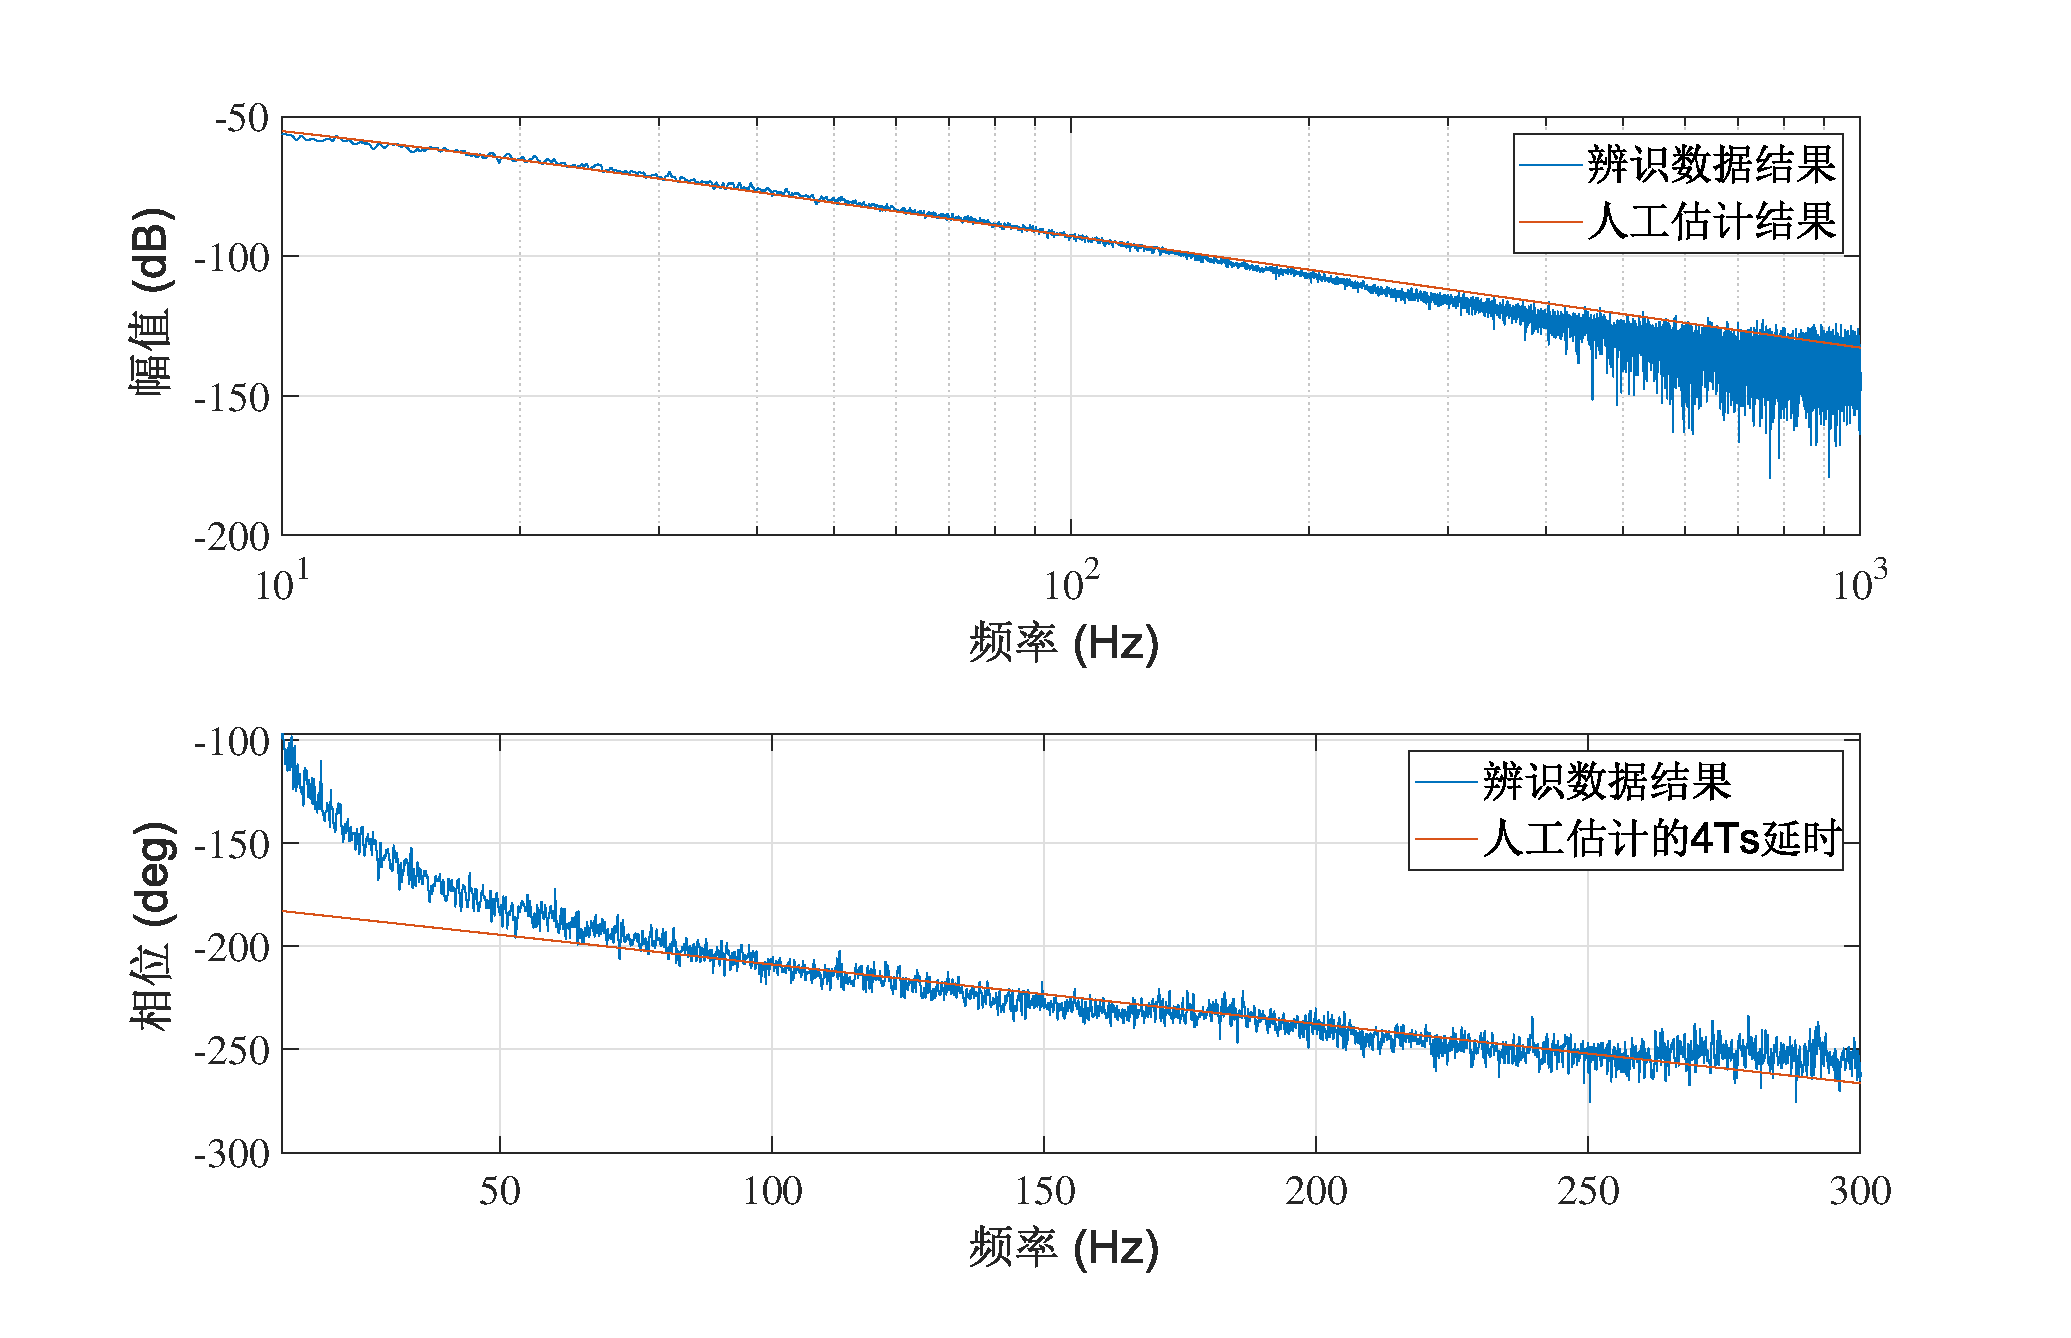
\includegraphics[width=12cm]{figures/辨识结果}
	\caption{辨识结果.}
	\label{辨识结果}
\end{figure}
图中,蓝色的线为实际辨识的数据,红色的线为辨识估计的数据。这里估计所采用的数学模型为最基础的二阶模型,如式(\ref{辨识公式})所示:
\begin{equation}
\label{辨识公式}
G(s)=\frac{1}{M_es^2+D_es}e^{-st_d}
\end{equation}
式中,由于辨识实际系统模型如图\ref{电机系统模型}所示,包含了驱动器部分,因此,辨识所得参数结果如下:

$M_e$为系统等效质量,这里为$\text{0.12$\,$Vs$^{2}$/m}$;

$D_e$为系统等效粘滞摩擦系数,这里为$\text{2.0$\,$Vs/m}$;

$t_d$为系统延时,这里为$\text{4$\,T_s$}$,即$\text{0.0008$\,$s}$。

从辨识结果来看,在300\,Hz以内,幅频曲线拟合的都比较好,超过300\,Hz,由于高频的未建模动态等因素,导致无法很好地拟合数据结果。相频曲线,从式(\ref{辨识公式})可知,估计采用的模型在$\text{s}$域内有两个极点,一个为0,另一个为$D_e/M_e$,即相位从-90°开始,在$\left|D_e/M_e\right|$\,Hz处下降90°,之后以斜率为$t_d$的直线变化,相对来说在300\,Hz以内,相频曲线较为理想。虽然高频无法很好地进行辨识,但辨识结果已经足以满足对于本文所涉及方法的要求,因为本文讨论的基于神经网络的一些方法对于模型的要求并不高,另外的一些补偿方法,也都会将模型的变化当做扰动的一种形式进行补偿。

此外,本文还对精密直线运动实验平台进行了定位力最大空间周期(即定位力的基频所对应的空间周期)的辨识,通过低速匀速运行,采集控制信号与位移信号,可以得到如图\ref{空间周期辨识}所示的结果,从图中很容易发现所标注的数据包含着定位力最大空间周期$\tau_{rip}=2\tau/3\,\text{mm}$的信息,其中$\tau$为实验平台PMLSM的极距($\tau=20\,\text{mm}$)。所标注出来的包含着几个非常常见的定位力的倍频所对应的空间周期,分别为$2\tau/3,\tau/3,\tau/4,\tau/6,2\tau/9$。
\begin{figure}[H]
	\centering
	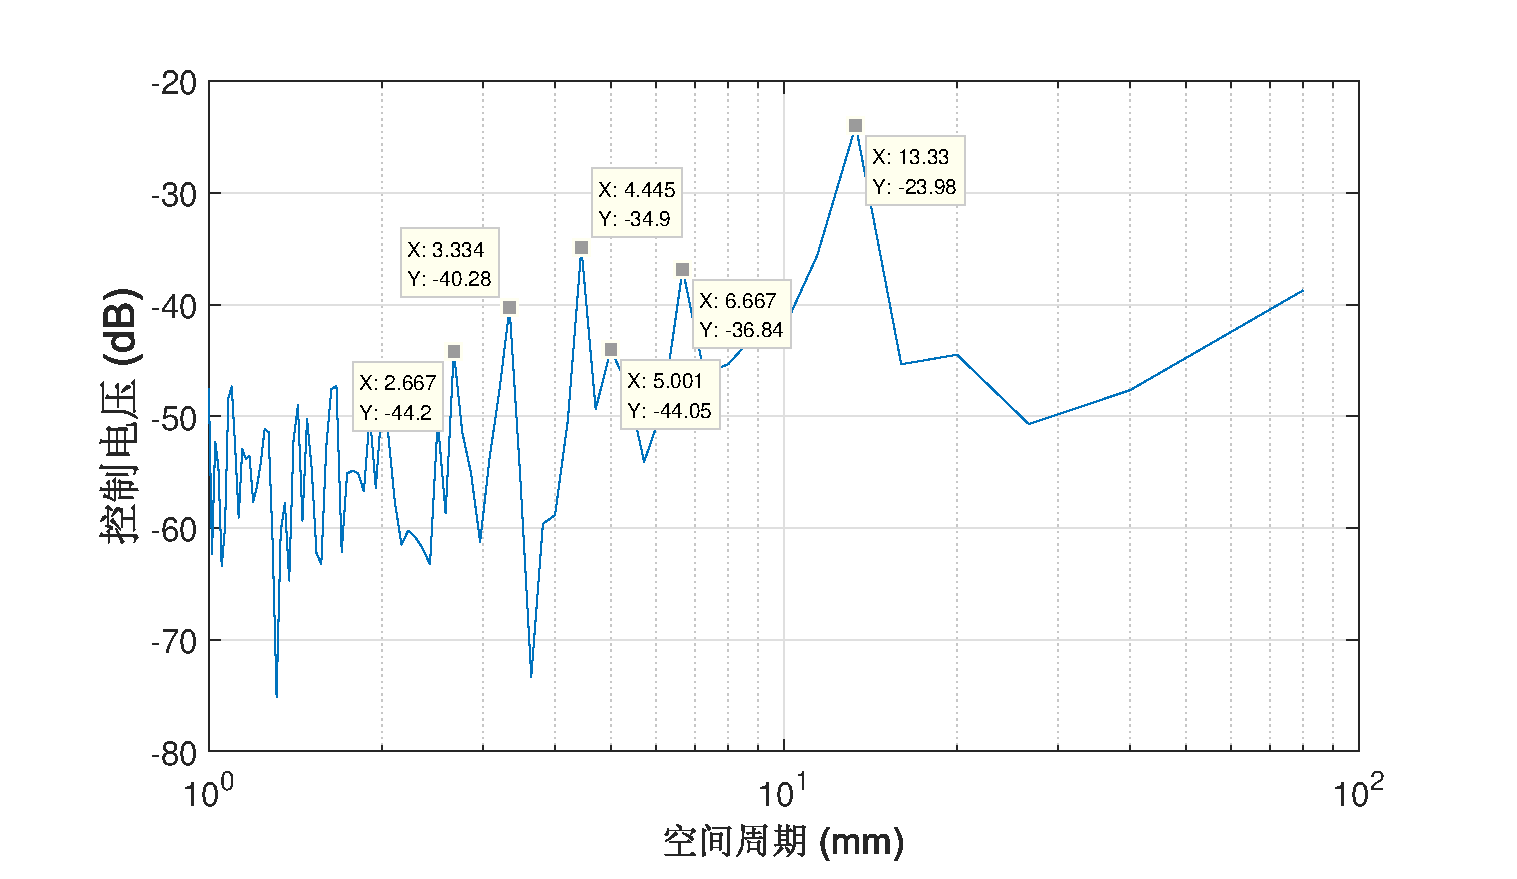
\includegraphics[width=12cm]{figures/空间周期辨识}
	\caption{定位力空间周期辨识.}
	\label{空间周期辨识}
\end{figure}
\section{本章小结}
本章首先介绍了精密直线运动平台系统工作原理,详细推导了PMLSMs的矢量变换控制原理。然后对精密直线运动平台动力学模型进行了详细介绍并提出了改进的扰动模型,其中,将系统扰动以集总扰动的形式进行了建模,为了方便后文控制方法的提出,进一步根据PMLSMs系统的特性,将集总扰动分为了时变的和时不变的两部分。此外,详细介绍了基于频率响应函数的系统辨识方法,详细介绍了离线开环辨识、闭环辨识和半闭环辨识三种辨识控制架构,并基于离线半闭环辨识控制架构对实验对象进行了辨识,得到了系统等效质量为$\text{0.12$\,$Vs$^{2}$/m}$,系统等效粘滞摩擦系数
为$\text{2.0\,Vs/m}$,系统延时为$\text{0.8$\,$ms}$,还对系统定位力的周期特性进行了辨识,得到其最大空间周期约为$13.33\,\text{mm}$,还可以发现,定位力的周期特性中,包含了2倍频、4倍频和6倍频的位置依赖扰动。这里系统模型特性为后续控制方法的研究提供了很好的基础。

\chapter{基于递推最小二乘的积分滑模控制方法研究}
\section{引言}
从第二章分析中可以知道,精密直线运动平台本质上也是一种非线性系统,尤其是其摩擦力、定位力、模型参数摄动、纹波扰动以及外部不确定扰动等均呈现出一定的非线性特性,因此,采用非线性的反馈控制器提高精密直线运动平台系统的整体控制性能显得很有必要,尤其是在超精密运动控制领域,抑制上述扰动带来的影响是提高运动控制性能的关键环节。近年来,滑模控制由于其控制律中含有具有开关特性的鲁棒项(符号函数及其变种),在处理PMLSMs诸多扰动因素时表现出优势\cite{wang2015modified,slotine1983tracking,burton1986continuous,tseng2010chattering,zhang2013design,lee2017adaptive}。但是,符号函数在原点附近的不连续会造成抖振,甚至可能造成系统不稳定或激发更多的不期望的模态,严重影响精密直线运动平台系统位置跟踪精度\cite{tseng2010chattering}。另一方面,由于缺乏对系统扰动的精确建模,传统的滑模控制方法在高速、高精度运动控制系统中不能完全满足要求,往往需要与额外的扰动补偿方法相结合。在精密直线运动平台控制系统中,前馈控制常常与反馈控制相结合,前者主要用来提高系统跟踪精度和补偿系统扰动,后者常用来维持系统稳定并一定程度上抑制系统的扰动,提高系统稳态精度。对于精密运动控制领域经常采用的三阶轨迹来说,前馈控制器主要在加减速段发挥作用,而反馈控制器主要在匀速段发挥作用。经典的前馈控制方法主要是基于系统的逆模型,但是往往需要提前辨识系统的模型,而且对模型辨识的精度要求极高,对于复杂的系统往往很难做到精确辨识,因此自适应的逆模型前馈控制显得很有必要。

本章首先介绍了滑模控制和递推最小二乘(Recursive Least Square, RLS)算法的基本原理,然后用积分滑模控制(Integral Sliding Mode Control, ISMC)作为反馈部分,用RLS实现逆模型的自适应前馈控制。为了能够补偿定位力带来的扰动,进一步对基于RLS的自适应逆模型前馈方法进行了改进,提出了一种基于改进型RLS的积分滑模控制方法,该方法将定位力的主要频率部分引入到RLS的回归向量中,从而进一步提高系统位置跟踪精度。
\section{滑模控制基本原理}
考虑单输入动态系统\cite{slotine2006应用非线性控制}
\begin{equation}
\label{4单输入动态系统}
x^{(n)}=f(\textbf{\textit{x}})+b(\textbf{\textit{x}})u
\end{equation}
式中,标量$x$是控制系统输出(如精密直线运动平台的位置),标量$u$是控制信号输入(比如电机的出力),向量$\textbf{\textit{x}}=[x,\dot{x},\dots,x^{n-1}]^T$为状态向量。$f(\textbf{\textit{x}})$通常表示一个非线性函数,用来表示系统的扰动,虽然不能精确知道,但一般都认为它的上界是$\textbf{\textit{x}}$的连续函数。$b(\textbf{\textit{x}})$也认为不能精确已知,但是其不确定性也认为是有界的,比如PMLSMs模型参数摄动等。

为了使有限控制$u$实现较为理想的跟踪任务,系统的期望状态的初始值$\textbf{\textit{x}}_d(0)$必须满足
\begin{equation}
\label{初态}
\textbf{\textit{x}}_d(0)=\textbf{\textit{x}}(0)
\end{equation}
即当$t=0$时控制系统输出与目标轨迹一致,这一条件在实际精密运动控制中基本都会满足,因为系统的位置和速度不会突变。

记跟踪误差为$e=x_d-x$,则跟踪误差向量为 $\textbf{\textit{e}}=\textbf{\textit{x}}_d-\textbf{\textit{x}}=[e \quad\dot {e} \quad\cdots \quad e^{n-1}]^T$。用标量方程$s(\textbf{\textit{e}};t)=0$定义n维状态空间中的滑模曲面$S(t)$
\begin{equation}
\label{滑模面0}
s(\textbf{\textit{e}},t)=\left(\frac{\text{d}}{\text{dt}}+\lambda\right)^{n-1}\textbf{\textit{e}}
\end{equation}
式中,$\lambda$为一正常数。$n$表示系统的阶数,比如机械系统,大部分会是二阶系统,即$n=2$,此时
\begin{equation}
\label{滑模面1}
s=\lambda e+\dot{e}
\end{equation}
即$s$仅是状态轨迹,即系统跟踪位置误差和速度误差的线性加权;$\lambda$为一正常数。


给定初始状态(\ref{初态}),跟踪问题$\textbf{\textit{x}}\equiv\textbf{\textit{x}}_d$则等价于当$t$\textgreater$0$时,通过一定的控制手段使系统状态轨迹能够始终停留在曲面$S(t)$上。实际上$s\equiv0$本质上为一种线性微分方程的表示,假定系统状态轨迹的初态满足式(\ref{初态}),则其唯一解为$\tilde{\textbf{\textit{x}}}\equiv0$。因此,通过一定的控制方式实现跟踪$n$维向量$\textbf{\textit{x}}_d$的问题可巧妙地转化为如何使标量$s$恒为零的问题。

更进一步,通过选择式(\ref{4单输入动态系统})中的控制信号$u$,使得状态轨线在曲面$S(t)$之外满足下式
\begin{equation}
\label{收敛条件}
\frac{1}{2}\frac{\text{d}}{\text{dt}}s^2\leq-\eta\left|s\right|
\end{equation}
从而保证$s$恒为零的问题简化为一阶问题,其中$\eta$为一正常数。如图\ref*{滑动条件}所示,系统状态轨线只要能够满足式(\ref{收敛条件}),系统状态轨线就会不断趋向于曲线$S(t)$,曲面$S(t)$就可以认为是一个不变集。系统状态轨线沿曲面$S(t)$运动的状态我们称为滑动模态。
%满足式(\ref{收敛条件})的曲面$S(t)$称为滑动曲面,当系统状态轨迹进入滑动曲面后,我们可以说系统进入了滑动模态,或滑动模。
\begin{figure}[H]
	\centering
	\includegraphics[width=10cm]{figures/滑动条件.pdf}
	\caption{滑动条件}
	\label{滑动条件}
\end{figure}
\begin{comment}
实际上,即使式(\ref*{初态})不满足,即初始时刻,系统输出与系统目标轨迹不一致,也就是说,系统不满足零状态,系统轨线仍然能够在小于$s(t=0)/\eta$的有限时间内到达曲面$S(t)$。总的来说,这种通过设计滑模面$S(t)$,并合理设计控制律$u$以使系统状态轨迹收敛到滑模面上的方法,成为滑模控制,是一种有效的容易实现的鲁棒控制方法。
\end{comment}
\section{递推最小二乘原理}
在介绍递推最小二乘原理之前,有必要先介绍最小二乘法。最小二乘法主要解决的问题是,对于像式(\ref{最小二乘})一样的表示,
\begin{equation}
\label{最小二乘}
y=\left[\begin{matrix}
x_{1} & \cdots & x_{n}
\end{matrix}\right]\left[\begin{matrix}
\theta_{1} \\
\vdots \\
\theta_{n}
\end{matrix}\right]
\end{equation}
其中$x$和$y$为一系列观测得到的数据,通过观测得到的$x$和$y$,求解其对应的估计参数$\symbf{\Theta}$的过程。可以用矩阵表示如下
\begin{equation}
\left[\begin{matrix}
y_{1} \\
\vdots \\
y_{k}
\end{matrix}\right]=\left[\begin{matrix}
\symbf{\phi}_{1}^{T} \\
\vdots \\
\symbf{\phi}_{k}^{T}
\end{matrix}\right] \symbf{\Theta}
\end{equation}
式中,
$k$表示观测到的数据个数;
$\symbf{\phi}_{i}^{T}=\left[\begin{matrix}x_{1}^{i} & \cdots & x_{n}^{i}\end{matrix}\right] \in \mathbb{R}^{1 \times n}$,表示第$i$组观测数据的输入量;

$y_i$表示第$i$组观测数据的输出量;

$\symbf{\Theta}=\left[\begin{matrix}\theta_{1} \\ \vdots \\ \theta_{n}\end{matrix}\right] \in \mathbb{R}^{n \times 1}$,为待估计参数。

记$\symbf{\Phi}_{k}=\left[\begin{matrix}\symbf{\phi}_{1}^{T} \\ \vdots \\ \symbf{\phi}_{k}^{T}\end{matrix}\right] \in \mathbb{R}^{k \times n}, \symbf{Y}_{k}=\left[\begin{matrix}y_{1} \\ \vdots \\ y_{k}\end{matrix}\right] \in \mathbb{R}^{k \times 1}$,则有
\begin{equation}
\label{3.8}
\symbf{\Phi}_{k}^{T}\left(\symbf{Y}_{k}-\symbf{\Phi}_{k} \hat{\symbf{\Theta}}_{k}\right)=0
\end{equation}
则通过方程(\ref{3.8}),即可求得最小二乘参数$\symbf{\Theta}_k$的估计,
\begin{equation}
\label{3.9}
\hat{\symbf{\Theta}}_{k}=\left(\symbf{\Phi}_{k}^{T} \symbf{\Phi}_{k}\right)^{-1} \symbf{\Phi}_{k}^{T} \symbf{Y}_{k}
\end{equation}
通过上述过程,可以发现,如果我们能够得到$x$和$y$的观测值,我们可以通过最小二乘方法求出$y$和$x$之间的函数关系。但是最小二乘法要求计算之前就能够得到所有的观测值,也就是说所有的数据都要提前准备好,这要求较大的存储空间,也影响计算速度,不利于实时在线的计算和补偿。因此,递推最小二乘应运而生。

递推最小二乘原理的根本目的是希望能够得到一种估计值的递推形式,比如$\hat{\symbf{\Theta}}_k=\hat{\symbf{\Theta}}_{k-1}+\Delta\hat{\symbf{\Theta}}_k$。下面是详细的推导过程:

最小二乘法的一般解如式(\ref{3.9})所示,这里分别表示$\symbf{\Phi}_{k}^{T} \symbf{\Phi}_{k}$和$\symbf{\Phi}_{k}^{T} \symbf{Y}_{k}$,令$\symbf{P}_{k}^{-1}=\symbf{\Phi}_{k}^{T} \symbf{\Phi}_{k}$,则有
\begin{equation}
\label{公式1}
\begin{aligned}
\symbf{\Phi}_{k}^{T} \symbf{\Phi}_{k}&=\left[\begin{matrix}
\symbf{\phi}_{1} & \cdots & \symbf{\phi}_{k}
\end{matrix}\right]\left[\begin{matrix}
\symbf{\phi}_{1}^{T} \\
\vdots \\
\symbf{\phi}_{k}^{T}
\end{matrix}\right]\\
&=\sum_{i=1}^{k} \symbf{\phi}_{i} \symbf{\phi}_{i}^{T}\\
&=\sum_{i=1}^{k-1} \symbf{\phi}_{i} \symbf{\phi}_{i}^{T}+\symbf{\phi}_{k} \symbf{\phi}_{k}^{T}\\
&=\symbf{P}_{k-1}^{-1}+\symbf{\phi}_{k} \symbf{\phi}_{k}^{T}
\end{aligned}
\end{equation}
同时,
\begin{equation}
\label{公式2}
\begin{aligned}
\symbf{\Phi}_{k}^{T} \symbf{Y}_{k}&=\left[\begin{matrix}
\symbf{\phi}_{1} & \cdots & \symbf{\phi}_{k}
\end{matrix}\right]\left[\begin{matrix}
y_{1} \\
\vdots \\
y_{k}
\end{matrix}\right]\\
&=\sum_{i=1}^{k} \symbf{\phi}_{i} y_{i}\\
&=\sum_{i=1}^{k-1} \symbf{\phi}_{i} y_{i}+\symbf{\phi}_{k} y_{k}\\
&=\symbf{\Phi}_{k-1}^{T} \symbf{Y}_{k-1}+\symbf{\phi}_{k} y_{k}
\end{aligned}
\end{equation}

此外,根据最小二乘法的一般解可以得到
\begin{equation}
\label{公式3}
\begin{matrix}
\hat{\symbf{\Theta}}_{k-1}=\left(\symbf{\Phi}_{k-1}^{T} \symbf{\Phi}_{k-1}\right)^{-1} \symbf{\Phi}_{k-1}^{T} \symbf{Y}_{k-1} \\
\Rightarrow \hat{\symbf{\Theta}}_{k-1}=\symbf{P}_{k-1} \symbf{\Phi}_{k-1}^{T} \symbf{Y}_{k-1} \\
\Rightarrow \symbf{P}_{k-1}^{-1} \hat{\symbf{\Theta}}_{k-1}=\symbf{\Phi}_{k-1}^{T} \symbf{Y}_{k-1}
\end{matrix}
\end{equation}

结合公式(\ref{公式1})$\sim$公式(\ref{公式3}),再次回顾最小二乘法的一般解,可以得出下面的推导
\begin{equation}
\begin{aligned}
\hat{\symbf{\Theta}}_{k}&=\left(\symbf{\Phi}_{k}^{T} \symbf{\Phi}_{k}\right)^{-1} \symbf{\Phi}_{k}^{T} \symbf{Y}_{k}\\
%&=\symbf{P}_{K} \symbf{\Phi}_{k}^{T} \symbf{Y}_{k}\\
&=\symbf{P}_{k}\left(\symbf{\Phi}_{k-1}^{T} \symbf{Y}_{k-1}+\symbf{\phi}_{k} \symbf{y}_{k}\right) \\
&=\symbf{P}_{k}\left(\symbf{P}_{k-1}^{-1} \hat{\symbf{\Theta}}_{k-1}+\symbf{\phi}_{k} \symbf{y}_{k}\right) \\
&=\symbf{P}_{k}\left[\left(\symbf{P}_{k}^{-1}-\symbf{\phi}_{k} \symbf{\phi}_{k}^{T}\right) \hat{\symbf{\Theta}}_{k-1}+\symbf{\phi}_{k} \symbf{y}_{k}\right] \\
%&=\hat{\symbf{\Theta}}_{k-1}-\symbf{P}_{k} \symbf{\phi}_{k} \symbf{\phi}_{k}^{T} \hat{\symbf{\Theta}}_{k-1}+\symbf{P}_{k} \symbf{\phi}_{k} \symbf{y}_{k}\\
&=\hat{\symbf{\Theta}}_{k-1}+\symbf{P}_{k} \symbf{\phi}_{k}\left(y_{k}-\symbf{\phi}_{k}^{T}\hat{\symbf{\Theta}}_{k-1}\right)\\
&=\hat{\symbf{\Theta}}_{k-1}+\symbf{K}_{k} \varepsilon_{k}\\
\end{aligned}
\end{equation}
至此,估计参数写成了$\hat{\symbf{\Theta}}_{k}=\hat{\symbf{\Theta}}_{k-1}+\Delta\symbf{\Theta}$的形式,其中$\Delta\symbf{\Theta}=\symbf{K}_k\varepsilon_{k}$。

综合上述的推导过程,这里可以进一步地给出递推最小二乘法的原理公式:
\begin{equation}
\label{RLS}
\left\{
\begin{aligned}
\hat{\symbf{\Theta}}_{k}&=\hat{\symbf{\Theta}}_{k-1}+\symbf{K}_{k} \varepsilon_{k}\\
\symbf{K}_{k}&=\symbf{P}_{k} \symbf{\phi}_{k}\\
\varepsilon_{k}&={y_{k}}-{\symbf{\phi}_{k}^{T} \hat{\symbf{\Theta}}_{k-1}}\\
\symbf{P}_{k}&=\left(\symbf{P}_{k-1}^{-1}+\symbf{\phi}_{k} \symbf{\phi}_{k}^{T}\right)^{-1}
\end{aligned}
\right.
\end{equation}
这里需要说明的是,$y_k$为标量、$\symbf{\phi}_{k}^{T}$、$\symbf{\Theta}_k$、$\symbf{\Theta}_{k-1}$都为向量。值得注意的是,公式(\ref{RLS})还无法通过编程实现递推最小二乘算法进行参数$\symbf{\Theta}$的估计。还要对其中的$\symbf{P}_k$进行进一步地求解。这里首先给出一个矩阵引逆定理(证明略):
假设矩阵$\symbf{A}\in \mathbb{C}^{N\times N}$,$\symbf{C}\in\mathbb{C}^{N\times N}$,均为非奇异矩阵,矩阵$\symbf{B}\in\mathbb{C}^{N\times M}$,$\symbf{D}\in\mathbb{C}^{M\times N}$,则矩阵$\symbf{A}+\symbf{BCD}$具有逆矩阵:
\begin{equation}
\label{引逆定理}
[\symbf{A}+\symbf{B C D}]^{-1}=\symbf{A}^{-1}-\symbf{A}^{-1} \symbf{B}\left[\symbf{C}^{-1}+\symbf{D} \symbf{A}^{-1} \symbf{B}\right]^{-1} \symbf{D} \symbf{A}^{-1}
\end{equation}
根据矩阵引逆定理(\ref{引逆定理}),
设 $\symbf{A}=\symbf{P}_{K-1}^{-1}, \symbf{B}=\symbf{\phi}_{k}, \symbf{C}=1, \symbf{D}=\symbf{\phi}_{k}^{T}$
则有
\begin{equation}
\label{逆}
\begin{aligned}
\symbf{P}_{k}&=\left(\symbf{P}_{k-1}^{-1}+\symbf{\phi}_{k} \symbf{\phi}_{k}^{T}\right)^{-1}\\
&=[\symbf{A}+\symbf{B C D}]^{-1}\\
&=\symbf{A}^{-1}-\symbf{A}^{-1} \symbf{B}\left[\symbf{C}^{-1}+\symbf{D} \symbf{A}^{-1} \symbf{B}\right]^{-1} \symbf{D} \symbf{A}^{-1}\\
&=\symbf{P}_{k-1}-\symbf{P}_{k-1} \symbf{\phi}_{k}\left[1+\symbf{\phi}_{k}^{T} \symbf{P}_{k-1} \symbf{\phi}_{k}\right]^{-1} \symbf{\phi}_{k}^{T} \symbf{P}_{k-1}\\
&=\symbf{P}_{k-1}-\frac{\symbf{P}_{k-1} \symbf{\phi}_{k} \symbf{\phi}_{k}^{T} \symbf{P}_{k-1}}{1+\symbf{\phi}_{k}^{T} \symbf{P}_{k-1} \symbf{\phi}_{k}}
\end{aligned}
\end{equation}

将式(\ref{逆})带入式(\ref{RLS}),可以得到最终的递推最小二乘算法:
\begin{equation}
\label{RLS1}
\left\{
\begin{aligned}
\hat{\symbf{\Theta}}_{k}&=\hat{\symbf{\Theta}}_{k-1}+\symbf{K}_{k} \varepsilon_{k}\\
\symbf{K}_{k}&=\symbf{P}_{k} \symbf{\phi}_{k}\\
\varepsilon_{k}&={y_{k}}-{\symbf{\phi}_{k}^{T}\hat{\symbf{\Theta}}_{k-1}}\\
\symbf{P}_{k}&=\symbf{P}_{k-1}-\frac{\symbf{P}_{k-1} \symbf{\phi}_{k} \symbf{\phi}_{k}^{T} \symbf{P}_{k-1}}{1+\symbf{\phi}_{k}^{T} \symbf{P}_{k-1} \symbf{\phi}_{k}}
\end{aligned}
\right.
\end{equation}
其中,

$y_k$为输出观测值;

$\symbf{\phi}_k$为输入观测向量,也称回归向量;

$\hat{\symbf{\Theta}}_{k}$为待估计参数向量;

$\symbf{P}_k$为更新律。
至此,所得到的递推最小二乘算法可以直接通过编程实现。


\section{基于传统递推最小二乘的前馈控制器设计}
在光刻机工件台与掩模台运动控制系统中,由于高分辨率和高产率的需求,常常希望精密直线运动平台加速段的精度更高、整定时间更短,这时,往往只靠反馈控制器不能很好地实现这一目的,因此,将前馈补偿与反馈控制相结合成为了一种较为流行的控制架构。经典的前馈补偿方式为系统逆模型前馈,通过事先辨识好系统的模型参数,然后通过逆模型前馈的方式计算得到需要的力。但是这种方式,需要对模型参数事先进行辨识,而且要求的辨识精度较高,往往需要付出额外的人力物力成本。一种较好的策略是通过在线自适应的方式调整系统的逆模型前馈参数\cite{butler2012adaptive},这样对于提前辨识的参数精度要求不高,只需要一个粗略的初始值即可实现逆模型自适应前馈控制,本节重点研究基于递推最小二乘方法进行逆模型自适应前馈的策略,并将之与积分滑模控制相结合,实现精密直线运动平台的高性能控制。

传统递推最小二乘积分滑模系统控制框图如图\ref{传统RLS}所示,主要包含自适应逆模型前馈与积分滑模反馈两部分,下面具体介绍基于传统递推最小二乘的前馈控制器的设计。
% TODO: \usepackage{graphicx} required
\\
\begin{figure}[H]
	\centering
	\includegraphics[width=12cm]{figures/RLSISMC2.pdf}
	\caption{传统递推最小二乘的积分滑模控制系统框图}
	\label{传统RLS}
\end{figure}

%\subsection{基于传统递推最小二乘的前馈控制器设计}

以经典的集中质量模型$1/(M_es^2+D_es+K_e)$为例,逆模型前馈控制信号可以表示为
\begin{equation}
\label{传统逆模型前馈}
u_{ff}=(M_es^2+D_es+K_e)p_d
\end{equation}
式中,$p_d$为系统位置参考轨迹。$M_e$、$D_e$和$K_e$为系统逆模型待确定的参数,$s$为拉普拉斯算子,表示微分。

如果将逆模型待确定的参数表示为向量的形式$\symbf{\Theta}=[M_e\,\, D_e\,\, K_e]^{T}$,则根据式(\ref{RLS1}),$\symbf{\Theta}$可以被估计为
\begin{equation}
\label{3.20}
\hat{\symbf{\Theta}}_{k}=\hat{\symbf{\Theta}}_{k-1}+\symbf{P}_{k} \symbf{\phi}_{k}\varepsilon_{k}
\end{equation}
式中,

$\hat{\symbf{\Theta}}_{k}$表示待确定参数向量的估计值;

$\symbf{P}_k$为自适应更新律,为一矩阵,可以表示为$\symbf{P}_{k}=\symbf{P}_{k-1}-\frac{\symbf{P}_{k-1} \symbf{\phi}_{k} \symbf{\phi}_{k}^{T} \symbf{P}_{k-1}}{1+\symbf{\phi}_{k}^{T} \symbf{P}_{k-1}\symbf{\phi}_{k}}$;

$\symbf{\phi}_{k}$为递推最小二乘的回归向量,即基向量,可以表示为$\symbf{\phi}_{k}=\left[\frac{d^{2} p_d}{d t^{2}} \,\,\frac{d p_d}{d t} \,\,p_d \right]^{T}$,这里指系统的三阶参考轨迹;

$\varepsilon_{k}$表示估计误差。

一旦$\symbf{\Theta}_k$的估计值$\hat{\symbf{\Theta}_k}$得到,就可以通过计算得出前馈控制器的估计输出指令
\begin{equation}
\label{3.21}
\hat{u_{ff}}=\hat{\symbf{\Theta}_k}^{T}\symbf{\phi}_{k}
\end{equation}
理想前馈控制器输出指令与估计得到的输出指令之间的差值可以表示为
\begin{equation}
\label{3.22}
\varepsilon_{k}^{'}=u_{ff}-\hat{u_{ff}}=\left[\symbf{\Theta}_k-\hat{\symbf{\Theta}_k}\right]^{T}\symbf{\phi}_{k}
\end{equation}
结合式(\ref{3.20})和式(\ref{3.22})以及文献\cite{landau1980extension}中定理2.1所表示的系统,$\varepsilon_{k}^{'}$又可假设为
\begin{equation}
\label{3.23}
\varepsilon_{k}^{'}=u_{ff}-\hat{u_{ff}}=Q\left[\Theta_k-\hat{\Theta_{k}}\right]^{T}\phi_{k}
\end{equation}
式中,$Q$为一离散的有理分式,根据波波夫超稳定性理论\cite{landau1980extension},如果$Q^{'}=Q-\frac{\lambda}{2}\,(0<\lambda<1)$严格正定,那么不管参数向量的估计初值$\hat{\symbf{\Theta}_0}$和自适应更新律初值$\symbf{P}_0$为何值,都有$\varepsilon_{k}^{'}$有界且
\begin{equation}
\label{3.24}
\lim _{k \rightarrow \infty} \varepsilon_{k}^{'}=0
\end{equation}

根据式(\ref{3.22})和式(\ref{3.23}),不难发现,在这里离散的有理传递函数$Q=1$,而且$Q^{'}=Q-\frac{\lambda}{2}>\frac{1}{2}$严格正定,因此,基于式(\ref{3.25})的递推最小二乘估计算法能够保证估计参数的收敛性。从图\ref{RLSISMC}
中可以看到,自适应前馈部分并未包含在系统的反馈回路中,因此,只要能够保证自身参数的收敛性,基于递推最小二乘估计的自适应前馈部分并不影响整个系统的闭环稳定性,闭环稳定性完全由积分滑模控制部分决定。
\begin{comment}
\subsection{基于积分滑模的反馈控制器设计}

精密直线运动平台的系统模型如式(\ref{2.14})所示,
$$
\begin{aligned}
\ddot{p}&=({{A}_{n}}+\Delta A)u_{fb}+L \\
&={A}_{n}u_{fb}+H  
\end{aligned}
$$
这里假设总扰动$H$有界,即$H\le\mu$,$\mu$为一正常数。$u_{fb}$表示反馈控制指令。

定义系统位置跟踪误差为
\begin{equation}
\label{3.25}
e=p_d-p
\end{equation}
可以得到误差对时间的导数为
\begin{equation}
\label{3.26}
\dot{e}=\dot{p_d}-\dot{p}
\end{equation}
滑模控制部分的设计主要包括两部分:滑模面的设计和控制律的设计。
这里设计滑模面为含积分项的滑模面
\begin{equation}
\label{3.27}
s=\lambda e+\beta\int_{}^{}e\text{d}t+\dot{e}
\end{equation}
式中,$\lambda$和$\beta$均为正常数。

根据式(\ref{3.26})和(\ref{3.27}),可以得出滑模面对时间的一阶导数为
\begin{equation}
\label{3.28}
\begin{aligned}
\dot{s}&=\lambda \dot{e}+\beta e+\ddot{e} \\ 
&=\lambda\dot{e}+\beta e+{{{\ddot{p}}}_{d}}-\ddot{p} \\ 
&=\lambda \dot{e}+\beta e+{{{\ddot{p}}}_{d}}-{{A}_{n}}u_{fb}-H  
\end{aligned}
\end{equation}
这里考虑到系统状态轨线的初始状态可能与目标轨迹的初始状态不一致,即系统可能不是零状态,因此需要一定的到达阶段才能保证系统状态轨线收敛到滑模面,为了方便,选定到达阶段的趋近律为等速趋近律
\begin{equation}
\label{3.29}
\dot{s}=-\eta\text{sgn}(s)
\end{equation}
式中,

$\text{sgn}(\cdot)$为符号函数;

$\eta$为正常数,满足$\eta\ge\mu$,主要决定到达阶段的趋近速率以及滑模控制的鲁棒性。

另一方面,设计滑模控制律为
\begin{equation}
\label{3.30}
u_{fb}=\frac{1}{A_n}\left(\lambda \dot{e}+\beta e+\ddot{p_d}+\eta\text{sgn}(s)\right)
\end{equation}
将式(\ref{3.30})代入式(\ref{3.28}),可得
\begin{equation}
\label{3.31}
\dot{s}=-\eta \text{sgn}(s)-H
\end{equation}

如前面提到的,基于递推最小二乘的积分滑模控制系统的闭环稳定性取决于积分滑模控制部分,这里为了证明其稳定性,根据Lyapunov稳定性理论,选择Lyapunov函数
\begin{equation}
\label{3.32}
V=\frac{1}{2}s^2
\end{equation}
两边对时间求导,即可得
\begin{equation}
\label{3.33}
\dot{V}=s\dot{s}
\end{equation}
将式(3.31)代入(3.33)中可以得到
\begin{equation}
\label{3.34}
\begin{aligned}
\dot{V}&=-\eta s\text{sgn}(s)-sH\\
&=-\eta\left|s\right|-sH\\
&\leq-\eta\left|s\right|+\mu\left|s\right|\\
&\leq-(\eta-\mu)\left|s\right|\\
&\leq 0
\end{aligned}
\end{equation}
取$\dot{V}\equiv0$,则$s\equiv0$,由LaSalle不变集定理可知,当$t\to\infty,s\to0$。至此,积分滑模反馈控制部分的渐近稳定性得以证明,反馈控制部分也设计完毕。
\end{comment}

\section{基于改进型递推最小二乘的积分滑模控制器设计}
\begin{comment}
在精密直线运动平台中,采用传统的基于递推最小二乘的积分滑模控制方法能够提高系统的位置跟踪精度,尤其是基于递推最小二乘的自适应逆模型前馈,能够有效地提高加速段的跟踪精度,同时减小系统从加速段进入匀速段的整定时间。但是正如第二章讨论的一样,由于精密直线运动平台本身的诸多非线性因素的影响,要进一步地提高系统的位置跟踪精度和扰动抑制能力,仅依赖逆模型前馈的积分滑模控制还有改进的空间。
\end{comment}




本节重点针对精密直线运动平台的定位力带来的扰动,在自适应前馈阶段引入了定位力的最大空间周期对应的扰动,对原有递推最小二乘的回归向量进行了改进,改进后的回归向量为$\symbf{\phi}_{k}^{'}=\left[\frac{d^{2} p}{d t^{2}} \,\,\frac{d p}{d t} \,\,p \,\,\text{sin}\left(2\pi p/\tau_m\right)\,\,\text{cos}\left(2\pi p/\tau_m\right)\right]^{T}$,其中,$\tau_m=2\tau/3=40/3\,\text{mm}$。改进之后的递推最小二乘可以分为两个部分:一是逆模型前馈部分,主要用来提高系统的瞬态响应速度;另一个是定位力补偿部分,用来补偿位置依赖的扰动对位置跟踪精度的影响。两部分都通过改进的递推最小二乘估计方法进行自适应调节,改进递推最小二乘积分滑模控制系统框图如图\ref{RLSISMC}所示。下面详细地介绍各部分的设计过程。
\begin{figure}[H]
	\centering
	\includegraphics[width=12cm]{figures/RLSISMC系统框图.pdf}
	\caption{改进递推最小二乘积分滑模控制系统框图}
	\label{RLSISMC}
\end{figure}

\subsection{基于改进型递推最小二乘的前馈控制器设计}
在工程实际中,还存在一种带遗忘因子的递推最小二乘算法\cite{butler2012adaptive}:
\begin{equation}
\label{RLS2}
\left\{
\begin{aligned}
\hat{\symbf{\Theta}}_{k}&=\hat{\symbf{\Theta}}_{k-1}+\symbf{K}_{k} \varepsilon_{k}\\
\symbf{K}_{k}&=\symbf{P}_{k} \symbf{\phi}_{k}\\
\varepsilon_{k}&={y_{k}}-{\symbf{\phi}_{k}^{T}\hat{\symbf{\Theta}}_{k-1}}\\
\symbf{P}_{k}&=\frac{1}{\zeta}\left(\symbf{P}_{k-1}-\frac{\symbf{P}_{k-1} \symbf{\phi}_{k} \symbf{\phi}_{k}^{T} \symbf{P}_{k-1}}{\zeta+\symbf{\phi}_{k}^{T} \symbf{P}_{k-1} \symbf{\phi}_{k}}\right)
\end{aligned}
\right.
\end{equation}
式中,$\zeta$为遗忘因子,$0<\zeta<1$,一般取0.98$\sim$0.999。本节改进型递推最小二乘的自适应更新律即采用式(\ref{RLS2})中的更新律。


因为改进后的回归向量为$\symbf{\phi}_{k}^{'}=\left[\frac{d^{2} p}{d t^{2}} \,\,\frac{d p}{d t} \,\,p \,\,\text{sin}\left(2\pi p/\tau_m\right)\,\,\text{cos}\left(2\pi p/\tau_m\right)\right]^{T}$,其中,$\tau_m=2\tau/3=40/3\,\text{mm}$。
这里将待确定的参数向量表示为$\symbf{\Theta}^{'}=[M_e\,\, D_e\,\, K_e\,\,a_1\,\,b_1]^{T}$,则根据式(\ref{RLS1}),$\Theta$可以被估计为
\begin{equation}
\label{3.25}
\hat{\symbf{\Theta}_{k}^{'}}=\hat{\symbf{\Theta}_{k-1}^{'}}+\symbf{P}_{k}^{'} \symbf{\phi}_{k}^{'}\varepsilon_{k}^{'}
\end{equation}
%式中,
%
%$\hat{\Theta_{k}^{'}}$表示待确定参数向量的估计值;
%
%$P_k^{'}$为自适应更新律,为一矩阵,可以表示为$P_{k}^{'}=P_{k-1}^{'}-\frac{P_{k-1}^{'} \phi_{k}^{'} {\phi_{k}^{'}}^{T} P_{k-1}^{'}}{1+{\phi_{k}^{'}}^{T} P_{k-1}^{'}\phi_{k}^{'}}$;
%
%$\phi_{k}^{'}$为改进后的回归向量;
%
%$\varepsilon_{k}^{'}$表示估计误差。

一旦$\Theta_k^{'}$的估计值$\hat{\Theta_k^{'}}$得到,就可以通过计算得出前馈控制器的估计输出指令
\begin{equation}
\label{3.26}
\hat{u_{ff}^{'}}=\hat{\symbf{\Theta}_k^{'}}^{T}\symbf{\phi}_{k}^{'}
\end{equation}


\subsection{基于积分滑模的反馈控制器设计}

精密直线运动平台的系统模型如式(\ref{2.14})所示,
$$
\begin{aligned}
\ddot{p}&=({{A}_{n}}+\Delta A)u_{fb}+L \\
&={A}_{n}u_{fb}+H  
\end{aligned}
$$
这里假设总扰动$H$有界,即$H\le\mu$,$\mu$为一正常数。$u_{fb}$表示反馈控制指令。

定义系统位置跟踪误差为
\begin{equation}
\label{3.27}
e=p_d-p
\end{equation}
可以得到误差对时间的导数为
\begin{equation}
\label{3.28}
\dot{e}=\dot{p_d}-\dot{p}
\end{equation}
滑模控制部分的设计主要包括两部分:滑模面的设计和控制律的设计。
这里设计滑模面为含积分项的滑模面
\begin{equation}
\label{3.29}
s=\lambda e+\beta\int_{}^{}e\text{d}t+\dot{e}
\end{equation}
式中,$\lambda$和$\beta$均为正常数。

根据式(\ref{3.28})和(\ref{3.29}),可以得出滑模面对时间的一阶导数为
\begin{equation}
\label{3.30}
\begin{aligned}
\dot{s}&=\lambda \dot{e}+\beta e+\ddot{e} \\ 
&=\lambda\dot{e}+\beta e+{{{\ddot{p}}}_{d}}-\ddot{p} \\ 
&=\lambda \dot{e}+\beta e+{{{\ddot{p}}}_{d}}-{{A}_{n}}u_{fb}-H  
\end{aligned}
\end{equation}
这里考虑到系统状态轨线的初始状态可能与目标轨迹的初始状态不一致,即系统可能不是零状态,因此需要一定的到达阶段才能到达滑动模态,为了方便,选定到达阶段的趋近律为等速趋近律
\begin{equation}
\label{3.31}
\dot{s}=-\eta\text{sgn}(s)
\end{equation}
式中,

$\text{sgn}(\cdot)$为符号函数;

$\eta$为正常数,满足$\eta\ge\mu$,主要决定到达阶段的趋近速率以及滑模控制的鲁棒性。

另一方面,设计滑模控制律为
\begin{equation}
\label{3.32}
u_{fb}=\frac{1}{A_n}\left(\lambda \dot{e}+\beta e+\ddot{p_d}+\eta\text{sgn}(s)\right)
\end{equation}
将式(\ref{3.32})代入式(\ref{3.30}),可得
\begin{equation}
\label{3.33}
\dot{s}=-\eta \text{sgn}(s)-H
\end{equation}

如前面提到的,基于递推最小二乘的积分滑模控制系统的闭环稳定性取决于积分滑模控制部分,这里为了证明其稳定性,根据Lyapunov稳定性理论,选择Lyapunov函数
\begin{equation}
\label{3.34}
V=\frac{1}{2}s^2
\end{equation}
两边对时间求导,即可得
\begin{equation}
\label{3.35}
\dot{V}=s\dot{s}
\end{equation}
将式(\ref{3.33})代入式(\ref{3.35})中可以得到
\begin{equation}
\label{3.36}
\begin{aligned}
\dot{V}&=-\eta s\cdot\text{sgn}(s)-sH\\
&=-\eta\left|s\right|-sH\\
&\leq-\eta\left|s\right|+\mu\left|s\right|\\
&\leq-(\eta-\mu)\left|s\right|\\
&\leq 0
\end{aligned}
\end{equation}
取$\dot{V}\equiv0$,则$s\equiv0$,由LaSalle不变集定理可知,当$t\to\infty,s\to0$。至此,积分滑模反馈控制部分的渐近稳定性得以证明,反馈控制部分也设计完毕。

最终得到的基于改进型递推最小二乘的积分滑模控制律可以表示为
\begin{equation}
\label{改进的控制律}
u=u_{ff}^{'}+u_{fb}
\end{equation}
式中,

$u_{ff}^{'}=u_{IM}+u_{fr}$表示总的前馈控制指令,包括逆模型自适应和定位力补偿自适应;

$u_{fb}$表示积分滑模反馈控制指令。
至此,基于改进型递推最小二乘的积分滑模控制方法设计完毕。
\section{本章小结}
本章为了提高精密直线运动平台的位置跟踪精度,首先研究了传统的基于递推最小二乘的自适应前馈补偿方法,该方法主要通过自适应系统逆模型来实现自适应前馈控制。另外,提出了一种基于改进型递推最小二乘的积分滑模控制方法,该方法充分考虑了精密直线运动平台定位力扰动带来的影响,将定位力的模型引入改进型递推最小二乘方法的回归向量中,并采用带有遗忘因子的更新律,实现了自适应前馈补偿,并与积分滑模反馈控制相结合,完成了基于改进型递推最小二乘的积分滑模控制方法设计,闭环系统的稳定性在Lyapunov稳定性理论的框架下进行了证明。






\chapter{基于神经网络的滑模控制方法研究}
\section{引言}很多的扰动补偿方法已经用于改善经典滑模控制方法,比如第三章提到的递推最小二乘法,还有干扰观测器以及神经网络补偿器等。其中,神经网络由于其不要求系统模型信息,在扰动补偿方面备受关注。但是在实际被控对象模型信息或者说扰动形式能够预先知道的情况下,加入特定的模型信息能够加快神经网络的收敛速度,进一步提高系统的扰动补偿能力。所以本节将精密直线运动平台系统特性引入到神经网络核函数的设计中,以提高系统的扰动补偿能力。

本章首先介绍了基于径向基函数(Radial Basis Function, RBF)神经网络的自适应补偿器设计,然后充分考虑精密直线运动平台的系统特性,提出了一种基于多核神经网络的动态边界层滑模控制方法,将精密直线运动平台定位力、摩擦力的经典模型考虑到神经网络核函数的设计中,进一步提高系统的位置跟踪性能和扰动抑制能力。
\begin{comment}
%\section{滑模控制基本原理}
考虑单输入动态系统\cite{slotine2006应用非线性控制}
\begin{equation}
\label{4单输入动态系统}
x^{(n)}=f(\textbf{x})+b(\textbf{x})u
\end{equation}
式中,标量$x$是控制系统输出(如精密直线运动平台的位置),标量$u$是控制信号输入(比如电机的出力),向量$\textbf{x}=[x,\dot{x},\dots,x^{n-1}]^T$为状态向量。$f(\textbf{x})$通常表示一个非线性函数,用来表示系统的扰动,虽然不能精确知道,但一般都认为它的上界是$\textbf{x}$的连续函数。$b(\textbf{x})$也认为不能精确已知,但是其不确定性也认为是有界的,比如PMLSMs模型参数慑动等。

为了使有限控制$u$实现跟踪任务,期望状态的初始值$\textbf{x}_d(0)$必须满足
\begin{equation}
\label{初态}
\textbf{x}_d(0)=\textbf{x}(0)
\end{equation}
即当$t=0$时控制系统输出与目标轨迹一致,这一条件在实际精密运动控制中基本都会满足,因为系统的位置和速度不会突变。

记跟踪误差为$e=x_d-x$,则跟踪误差向量为 $\textbf{e}=\textbf{x}_d-\textbf{x}=[e \quad\dot {e} \quad\cdots \quad e^{n-1}]^T$。用标量方程$s(\textbf{e};t)=0$定义状态空间$R_n$中的时变曲面$S(t)$
\begin{equation}
\label{滑模面0}
	s(\textbf{e};t)=\left(\frac{\text{d}}{\text{dt}}+\lambda\right)^{n-1}e
\end{equation}
式中,$\lambda$为一正常数。$n$表示系统的阶数,比如机械系统,大部分会是二阶系统,即$n=2$,此时
\begin{equation}
\label{滑模面1}
s=\lambda e+\dot{e}
\end{equation}
即$s$仅是位置误差和速度误差的加权和。
给定初始状态(\ref{初态}),跟踪问题$\textbf{x}\equiv\textbf{x}_d$则等价于当$t$\textgreater$0$时,使状态轨线停留在曲面$S(t)$上。实际上$s\equiv0$代表一个线性微分方程,假定初始条件为式(\ref{初态}),则其唯一解为$\tilde{\textbf{x}}\equiv0$。因此,跟踪$n$维向量$\textbf{x}_d$的问题可简化为标量$s$恒为零的问题。

更进一步,通过选择式(\ref{4单输入动态系统})中的控制信号$u$,使得状态轨线在曲面$S(t)$之外满足下式
\begin{equation}
\label{收敛条件}
\frac{1}{2}\frac{\text{d}}{\text{dt}}s^2\leq-\eta\left|s\right|
\end{equation}
从而保证$s$恒为零的问题简化为一阶问题,其中$\eta$为正常数。本质上,式(\ref{收敛条件})表示的是以$s^2$为度量到曲面的平方``距"沿所有系统轨线减小,因此系统轨线就会不断趋向于曲线$S(t)$。如图\ref*{滑动条件}所示,轨线只要能够进入曲面就会一直停留在该曲面上。从另一个角度来说,系统轨线满足式(\ref{收敛条件}),就会使曲面成为一个不变集。满足式(\ref{收敛条件})的曲面$S(t)$称为滑动曲面,且当系统状态在曲面上时就被称为滑动模或滑动形态。

实际上,即使式(\ref*{初态})不满足,即初始时刻,系统输出与系统目标轨迹不一致,也就是说,系统不满足零状态,系统轨线仍然能够在小于$s(t=0)/\eta$的有限时间内到达曲面$S(t)$。总的来说,这种通过设计滑模面$S(t)$,并合理设计控制律$u$以使系统状态轨迹收敛到滑模面上的方法,成为滑模控制,是一种有效的容易实现的鲁棒控制方法。
\begin{figure}
	\centering
	\includegraphics[width=10cm]{figures/滑动条件}
	\caption{滑动条件}
	\label{滑动条件}
\end{figure}
\end{comment}
%\section{基于传统RBF神经网络的滑模控制器设计}

\section{基于传统RBF神经网络的自适应补偿器设计}
%1985年,Powell提出了多变量插值的RBF方法。RBF是一个取值仅仅依赖于离原点距离的实值函数,也就是$\phi(x)=\phi(\norm{x})$,或者还可以理解为到任意一点$c$的距离,$c$点定义为中心点,也就是$\phi(x,c)=\phi(\norm{x-c})$。凡是满足$\phi(x)=\phi(\norm{x})$性质的函数$\phi$都可以称为RBF。经典的RBF一般使用欧氏距离(也叫做欧式RBF),尽管其他距离函数也可以满足RBF的定义。
%最常用的RBF神经网络是基于高斯核函数建立的,形式为
%
%\begin{equation}
%k\left(\norm{x-x_c}\right)=\text{exp}\left(\frac{-\norm{x-x_c}^2}{(2\sigma)^2}\right)
%\end{equation}
%其中,

%$x_c$为核函数中心点,类似于输入信号的平均值;
%
%$\sigma$为函数的宽度参数,类似于输入信号的标准差,决定了函数的径向作用范围。

传统的RBF神经网络凭借对于非线性函数强大的拟合能力\cite{1987Powell},常被用来作为前馈补偿器在线补偿精密直线运动平台的集总扰动,然后通过一定的规则对其权重参数进行在线调整。这里选用网络结构为1-5-1,如图\ref{RBF网络结构}所示。其中,$h_i\,(i=1,2,3,4,5)$表示隐含层5个高斯核函数节点。
\\
\begin{figure}[H]
	\centering
	\includegraphics[width=12cm]{figures/RBF神经网络结构.pdf}
	\caption{RBF网络结构}
	\label{RBF网络结构}
\end{figure}

RBF神经网络的算法可以表示为
\begin{equation}
\begin{aligned}
&h_i=\text{exp}\left(\frac{-\norm{x_i-c_i}^2}{2{b_i}^2}\right)\\
&H(x)={\textbf{\textit{W}}^{*T}}h(x)+\varepsilon\\
\end{aligned}
\end{equation}
式中,

$x_i$为第$i$个隐含层的输入;

$c_i$为第$i$个隐含层核函数中心点,类似于输入信号的平均值;

$b_i$为第$i$个隐含层核函数的宽度参数,类似于输入信号的标准差,决定了函数的径向作用范围;

$h(x)$为隐含层的输出;

$\textbf{\textit{W}}^*$为隐含层到输出层的理想权重;

$\varepsilon$为神经网络的逼近误差,$\left|\varepsilon\right| <{{\varepsilon }_{max}}$。

传统的RBF神经网络的输入选为精密直线运动平台的速度信号$\dot{p}$,网络输出为对$H$的估计
\begin{equation}
\hat{H}={\hat{\textbf{\textit{W}}}}^{T}h(\dot{p})
\end{equation}
式中,$\hat{\textbf{\textit{W}}}$为隐含层到输出层的估计权重,取$\tilde{\textbf{\textit{W}}}=\hat{\textbf{\textit{W}}}-\textbf{\textit{W}}^*$,则有
\begin{equation}
H-\hat{H}=-{{\tilde{\textbf{\textit{W}}}}^{T}}h+\varepsilon
\end{equation}
表示传统RBF神经网络估计值与理想值之间的差别。在实际的精密直线运动平台中,用$\hat{H}$来实现对系统集总扰动的在线补偿,即实现了基于传统RBF神经网络的补偿器。在设计流程中,重要的是确定网络结构以及高斯核函数的参数,即核函数中心点和宽度参数,这里都根据经验选取,即中心点假设根据输入信号均匀分布进行确定,宽度参数假设相邻中心点的差值。

\section{基于多核神经网络的动态边界层滑模控制器设计}
为了实现PMLSM的高性能控制,本文提出了一种带有动态边界层的多核神经网络滑模控制(Multi-Kernel Neural Network Sliding Mode Control, MNNSMC)方法。该方法采用多核神经网络对系统非线性扰动进行在线补偿。其中,核函数的设计不仅基于传统的高斯核函数,还引入了三角核函数和sigmoid核函数,极大程度地抑制了PMLSM定位力、摩擦力等各种不确定因素带来的影响,提高了系统的跟踪性和鲁棒性。另一方面,采用边界层可动态调整的饱和函数,不仅可以削弱抖振,还可以保证系统状态轨迹渐近收敛到切换平面。基于MNNSMC的PMLSM运动控制系统的控制框图如图\ref{MNNSMC控制架构}所示,下面具体介绍各部分的设计。
\begin{figure}[H]
	\centering
	\includegraphics[width=12cm]{figures/MNNSMC控制架构1.pdf}
	\caption{基于MNNSMC的PMLSMs控制系统框图}
	\label{MNNSMC控制架构}
\end{figure}

\begin{comment}
与基于传统RBF神经网络的滑模控制设计不同的部分在于神经网络和边界层的设计部分,分别如4.4.1节和4.4.2节所述,神经网络部分相比于传统的基于单核(高斯核函数)的RBF神经网络改进为考虑了PMLSMs扰动模型结构的多核神经网络(MNN),边界层部分将经典的固定边界层饱和函数改进为动态边界层饱和函数(DBSMC),稳定性的证明和多核神经网络权重的自适应律都是基于Lyapunov理论得出,最终得到的改进的控制律为
\begin{equation}
\label{4-29}
\begin{aligned}
U& =\frac{1}{{{B}_{n}}}\left[\lambda \dot{e}+{{{\ddot{p}}}_{d}}-\hat{H^{'}}+\eta \text{sat}\left(\frac{S(t)}{\Delta(\dot{p})}\right)\right] \\ 
& ={{U}_{eq}^{'}}+{{U}_{nn}^{'}} \\ 
\end{aligned}
\end{equation}
其中,
\begin{equation}
\label{4-30}
\begin{aligned}
U_{e q}^{'}&=\frac{1}{B_{n}}\left[\lambda \dot{e}+\ddot{p}_{d}+\eta \operatorname{sat}\left(\frac{S(t)}{\Delta(\dot{p})}\right)\right] \\
U_{n n}^{'}&=-\frac{1}{B_{n}} \hat{H^{'}}
\end{aligned}
\end{equation}
式中,
%\text{sat}\left(\frac{S(t)}{\Delta(\dot{p})}\right)

$U_{eq}^{'}$为含动态边界层的滑模控制律;

$U_{nn}^{'}$为多核神经网络补偿律;

$\hat{H^{'}}$为多核神经网络的输出,这里将多核神经网络的隐含层输出统一表示为$h^{'}(x)$,则$\hat{H^{'}}(x)$为
\begin{equation}
\label{4-31}
\hat{H^{'}}(x)={\mathbf{W}^{T}}h^{'}(x)
\end{equation}

多核神经网络隐含层到输出层权重的更新律可以表示
\begin{equation}
\label{4-32}
\dot{\hat{\bf{W^{'}}}}=-{{\textbf{ }\!\!{\gamma}\!\!\text{}}^{-1}}Sh^{'}(x)\text{,}
\end{equation}
至此,多核神经网络滑模控制器方法设计完毕。
\end{comment}

\subsection{多核神经网络补偿器设计}
神经网络对于非线性函数有着良好的拟合能力,在扰动补偿方面很受欢迎\cite{zhao2019adaptive,sun2019adaptive}。但是传统的神经网络往往是一个“黑箱模型”,在处理集总扰动时没有充分利用系统扰动的特性。

正如第二章讨论的一样,PMLSMs系统的定位力和摩擦力是扰动的主要来源,而且有很多经典的模型已经被提出,专门用来近似定位力和摩擦力,因此对其进行辨识和补偿可以在一定程度上提高精密直线运动平台的扰动抑制能力。这里充分利用PMLSMs系统扰动的一些特性,将定位力与摩擦力的经典模型考虑到神经网络核函数的设计中,提出了一种多核神经网络(Multi-Kernel Neural Network, MNN)补偿器,其结构如图\ref*{MNN结构}所示。该结构中保留了RBF神经网络经典的3层结构。隐含层中不仅用经典的高斯核函数补偿时变的扰动,如图中$f_1$,还引入了三角核函数,以及sigmoid核函数,分别对应补偿定位力和摩擦力带来的扰动,如图中$f_2$。三种核函数的具体形式为:
\\
\begin{figure}[H]
	\centering
	\includegraphics[width=12cm]{figures/MNN.pdf}
	\caption{多核神经网络结构}
	\label{MNN结构}
\end{figure}
\begin{enumerate}
	\item[A.] \textbf{高斯核函数}. 高斯核函数的数学描述为
	\begin{equation}
	{{h}_{j}}=\text{exp}(-\frac{{{({{x}_{j}}-{{c}_{j}})}^{2}}}{2b_{j}^{2}})
	\end{equation}
	式中,$h_j$为第$j$个高斯核函数的输出;$x_j$为第$j$个高斯核函数的输入;$c_j$,\,$b_j$分别为第$j$个高斯核函数的中心的宽度参数,统计学意义上分别相当于输入信号的均值和方差;$j$=1, 2, $\cdots$, $N_h$;$N_h$是高斯核函数的个数。
	\item[B.] \textbf{三角核函数}. 三角核函数的数学描述为
	\begin{equation}
	{{t}_{k}}=\left\{ \begin{aligned}
	&\text{sin}(\frac{2\text{ }\!\!\pi\!\!\text{ }{{n}_{k}}}{{{\tau }_{s}}}{{x}_{k}})\text{,} \\ 
	&\text{cos}(\frac{2\text{ }\!\!\pi\!\!\text{ }{{n}_{k}}}{{{\tau }_{s}}}{{x}_{k}})\text{,} \\ 
	\end{aligned} \right.
	\end{equation}
	式中,$t_k$是第$k$个三角核函数的输出;$x_k$是第$k$个三角核函数对的输入;$\tau_s$是PMLSMs定位力的基频所对应的空间周期;\,$n_k$是PMLSMs定位力的谐波次数,通常为1,2,4,6等;$k$=1, 2, $\cdots$, $N_t$;$N_t$是三角核函数对的个数。
	\item[C.]\textbf{sigmoid 核函数}. sigmoid核函数的数学描述为
	\begin{equation}
	{{g}_{r}}=\frac{1-\text{exp}(-{{x}_{r}})}{1+\text{exp}(-{{x}_{r}})}
	\end{equation}
	式中,$g_r$第$r$个sigmoid核函数的输出;$x_r$是第$r$个sigmoid核函数的输入; $r$=1, 2, $\cdots$, $N_r$;$N_r$是sigmoid核函数的个数。
\end{enumerate}

基于前文设计的多核神经网络结构,这里为了简化,将神经网络的输出统一表述为
\begin{equation}
H(x)={\textbf{\textit{W}}^{*T}}h(x)+\varepsilon
\end{equation}
式中,

$x$为各隐含层的输入;

$h(x)$为隐含层的输出;

$\textbf{\textit{W}}^*$为隐含层到输出层的理想权重。其中,$\varepsilon$为神经网络的逼近误差,$\left|\varepsilon\right|\le\varepsilon_{max}$。网络输出为对$H(x)$的估计
\begin{equation}
\hat{H}={\hat{\textbf{\textit{W}}}}^{T}h(x)
\end{equation}
式中,$\hat{\textbf{\textit{W}}}$为隐含层到输出层的估计权重,取$\tilde{\textbf{\textit{\textbf{\textit{W}}}}}=\hat{\textbf{\textit{W}}}-\textbf{\textit{W}}^*$,则有
\begin{equation}
H-\hat{H}=-{{\tilde{\bf{W}}}^{T}}h+\varepsilon
\end{equation}
\subsection{基于多核神经网络的滑模控制器设计}
如式(\ref{2.14})所示,PMLSMs系统模型为
\begin{equation}
\label{(4-10)}
\begin{aligned}
\ddot{p}&=({{A}_{n}}+\Delta A)U+L \\ 
&={A}_{n}U+H  
\end{aligned}
\end{equation}

定义系统位置跟踪误差为
\begin{equation}
\label{4-11}
e=p_d-p
\end{equation}
两边对时间求导,可以得到误差对时间的导数为
\begin{equation}
\label{4-12}
\dot{e}=\dot{p_d}-\dot{p}
\end{equation}
滑模控制部分的设计主要包括两部分:滑模面的设计和控制律的设计。
这里设计滑模面为
\begin{equation}
\label{4-13}
S=\lambda e+\dot{e}
\end{equation}
式中,$\lambda$为一正常数。

根据式(\ref{(4-10)})和(\ref{4-12}),可以得出滑模面对时间的一阶导数为
\begin{equation}
\label{4-14}
\begin{aligned}
\dot{S}&=\lambda \dot{e}+\ddot{e} \\ 
&=\lambda\dot{e}+{{{\ddot{p}}}_{d}}-\ddot{p} \\ 
&=\lambda \dot{e}+{{{\ddot{p}}}_{d}}-{{A}_{n}}U-H  
\end{aligned}
\end{equation}
这里考虑到系统状态轨线的初始状态可能与目标轨迹的初始状态不一致,即系统可能不是零状态,因此需要一定的到达阶段才能保证系统进入滑动模态,同样,这里选定到达阶段的趋近律为等速趋近律
\begin{equation}
\dot{S}=-\eta\text{sgn}(S)
\end{equation}
式中,
%$\text{sgn}(\cdot)$为符号函数;
$\eta$为正常数,与神经网络逼近误差之间满足$\eta\ge\left|\varepsilon_{max}\right|$,主要决定到达阶段的趋近速率。

根据(\ref{4-13})和(\ref{4-14}),可以得出基于多核神经网络的滑模控制器的控制律为
\begin{equation}
\label{4-16}
\begin{aligned}
U& =\frac{1}{{{B}_{n}}}[\lambda \dot{e}+{{{\ddot{p}}}_{d}}-\hat{H}+\eta \text{sgn} (S)] \\ 
& ={{U}_{eq}}+{{U}_{nn}} \\ 
\end{aligned}
\end{equation}
其中,
\begin{equation}
\label{4-17}
\begin{aligned}
U_{e q}&=\frac{1}{B_{n}}\left[\lambda \dot{e}+\ddot{p}_{d}+\eta \operatorname{sgn}(S)\right] \\
U_{n n}&=-\frac{1}{B_{n}} \hat{H}
\end{aligned}
\end{equation}
式中,
$U_{eq}$为滑模控制律;$U_{nn}$为神经网络补偿律。

为了证明整个控制系统的稳定性,同时获得多核神经网络隐含层到输出层的权重更新律,选择Lyapunov函数为
\begin{equation}
\label{4-18}
V=\frac{1}{2}{{S}^{2}}+\frac{1}{2}{{\tilde{\textbf{\textit{W}}}}^{T}}\symbf{\gamma}\tilde{\textbf{\textit{W}}}
\end{equation}
式中,$\symbf{\gamma}$为一对角阵,且元素均大于0。两边对时间求导,可得
\begin{equation}
\label{4-19}
\dot{V}=S \dot{S}+\tilde{\textbf{\textit{W}}}^{T}\symbf{\gamma} \dot{\tilde{\textbf{\textit{W}}}}
\end{equation}
结合式(4.9)、式(\ref{4-14})、式(\ref{4-16})、式(\ref{4-17})和式(\ref{4-19}),
\begin{equation}
\label{4-20}
\begin{aligned}
\dot{V}&=-\eta S\text{sgn}(S)+S{{{\tilde{\textbf{\textit{W}}}}}^{T}}h(x)-S\varepsilon +{{{\tilde{\textbf{\textit{W}}}}}^{T}}\symbf{\gamma}\dot{\hat{\textbf{\textit{W}}}} \\ 
&=-\eta S\text{sgn}(S)-S\varepsilon +{{{\tilde{\textbf{\textit{W}}}}}^{T}}(Sh(x)+\symbf{\gamma}\dot{\hat{\textbf{\textit{W}}}}) \\ 
&=-\eta \left| S \right|-S\varepsilon +{{{\tilde{\textbf{\textit{W}}}}}^{T}}(Sh(x)+\symbf{\gamma}\dot{\hat{\textbf{\textit{W}}}})\text{.} \\ 
\end{aligned}
\end{equation}
取自适应律为 
\begin{equation}
\label{4-21}
\dot{\hat{\textbf{\textit{W}}}}=-\symbf{\gamma}^{-1}Sh\text{,}
\end{equation}
将自适应律代入式(\ref{4-20}),可以得到
\begin{equation}
\label{4-22}
\dot{V}=-\eta\left|S\right|-S\varepsilon\le 0\text{.}
\end{equation}
式(\ref{4-22})中,取$\dot{V}\equiv0$,则$S\equiv0$,由LaSalle不变集定理可知,当$t\to\infty,S\to0$。因此,多核神经网络滑模控制器的渐近稳定性得以证明。

式(\ref{4-17})中的滑模控制律之所以有较强的鲁棒性,主要在于有切换功能的开关函数,但开关函数会引起控制信号较大的抖振,往往用原点附近连续的饱和函数替代原点附近不连续的开关函数以削弱抖振,传统的固定边界层饱和函数可表示为
\begin{equation}
\label{4-23}
\operatorname{sat}\left(\frac{S}{\Delta}\right)=\left\{\begin{array}{ll}
1 & \mathrm{~S} \geq \Delta \\
\frac{S}{\Delta} & -\Delta<S<\Delta \\
-1 & \mathrm{~S} \leq-\Delta
\end{array}\right.
\end{equation}
式中,$\Delta$为边界层厚度,其取值往往依靠经验选取,选取的值过大,可以削弱抖振,但同时会造成稳态误差,进而对位置跟踪精度产生影响;取值过小,则对于削弱抖振效果不明显\cite{jin2007investigation}。固定边界层如图\ref{固定边界层}所示,其中,$\Delta$为边界层宽度。从图\ref{固定边界层}中可知,切换平面$S=0$位于边界层中间,在边界层内部相当于线性控制,因此无法保证系统在边界层厚度内稳定,即$[-\Delta,\Delta]$区间内保证稳定,这就使得系统在边界层内不能快速的响应外界扰动,降低了鲁棒性,同时位置跟踪精度也无法保证渐近收敛到$0$。因此,设计新型的饱和函数,即能够保证系统状态轨迹渐近收敛到切换平面上的饱和函数有重要意义。具体的工作将在4.3.3节进行详细介绍。
\begin{figure}[H]
	\centering
	\includegraphics[width=12cm]{figures/固定边界层1.pdf}
	\caption{固定边界层}
	\label{固定边界层}
\end{figure}





\subsection{动态边界层设计}
如4.3.2节所述,设计新型饱和函数能够保证系统状态轨线渐近收敛到0,对于进一步提高PMLSMs系统位置跟踪精度具有重要意义。为了实现这一目的,边界层厚度随着系统状态轨迹变化而变化的饱和函数应运而生\cite{jin2007investigation},这里基于被控对象的系统特性,定义新型饱和函数为
\begin{equation}
\text{sat}\left(\frac{S(t)}{\Delta(\dot{p})}\right)=\left\{\begin{aligned}
&\frac{S(t)}{\Delta(\dot{p})} \quad&\left|\frac{S(t)}{\Delta(\dot{p})}\right|\le1\text{,} \\ 
&\text{sat}\left(\frac{S(t)}{\Delta(\dot{p})}\right) \quad&\left|\frac{S(t)}{\Delta(\dot{p})} \right|>1\text{,} \\ 
\end{aligned}\right.
\end{equation}
式中,$\Delta(\dot{p})$动态边界层厚度,考虑到PMLSMs系统位置跟踪误差与运动轨迹相关,在加减速段跟踪误差往往更大,需要更大的边界层厚度削弱抖振,匀速段跟踪误差相对较小。当系统状态轨迹到达边界层内部后,缩小边界层厚度可以保证系统状态轨迹渐近收敛到切换平面,进而保证位置跟踪误差渐近收敛到0。因此,本文将边界层厚度表示为系统输出速度的函数 
\begin{equation}
\Delta(\dot{p})={{\Delta}_{0}}(1-\alpha\left|{\dot{p}}\right|)
\end{equation}
式中,

$\Delta_0$为边界层厚度的初始值,即系统输出速度为0时的边界层厚度;

$\alpha$定义为边界层调节因子,为一非负常数。当系统到达边界层内时, $\Delta(\dot{p})$会逐渐减小,不断趋近于切换平面$S(t)$\,=\,0, $S(t)/\Delta(\dot{p})$的斜率会增加。当$\Delta(\dot{p})$\,$\to$\,0,$S(t)/\Delta(\dot{p})$的斜率无限增大,则新型饱和函数最终可以等效地看成开关函数 $\text{sgn}(\cdot)$,如图\ref{动态边界层}所示。因此,带有动态边界层的饱和函数即能够保证系统的快速切换,又能够保证原点附近的连续性,对削弱系统抖振和提高系统跟踪精度很有帮助。 
\begin{figure}[H]
	\centering
	\includegraphics[width=12cm]{figures/动态边界层1.pdf}
	\caption{动态边界层}
	\label{动态边界层}
\end{figure}

\section{本章小结}
本章针对神经网络在滑模控制器设计中的应用进行了深入研究,介绍了基于传统RBF神经网络的自适应补偿器,提出了一种新型的带有动态边界层的MNNSMC方法。该方法包含MNN和滑模控制两个部分,其中,MNN将PMLSMs扰动的经典模型结构考虑到神经网络核函数的设计中,分别用三角核函数和sigmoid核函数补偿定位力和摩擦力等时不变的扰动,同时保留传统RBF的高斯核函数补偿时变的非线性扰。另一方面,提出了一种动态边界层饱和函数以进一步提高系统的位置跟踪能力。最后,通过构建关于滑模变量与神经网络权重的李雅普诺夫函数,证明了带有动态边界层的MNNSMC的渐近稳定性,从理论上表明了所提方法对于提高精密直线运动平台位置跟踪性能和扰动抑制能力的有效性。
%\newpage
%\mbox{}
%\newpage
\chapter{精密直线运动平台控制系统实验验证与分析}
\section{引言}
为了充分说明本文所提IRLSISMC方法和MNNSMC方法的有效性,本章以精密直线运动平台为实验对象,在不同的参考轨迹输入情况下,拟进行一系列位置跟踪实验。同时,设计多种性能评价指标,将实验结果与同类型的传统控制方法进行比较,验证本文所提控制方法对精密直线运动平台位置跟踪性能和扰动抑制能力的改善效果。

\section{实验验证与分析}
\subsection{实验装置}
图\ref{精密直线运动平台实验装置}所示为基于Speedgoat实时系统的精密直线运动平台实验装置,包括PMLSM、PC、Speedgoat实时控制系统、光栅位移传感器以及Trust线性放大器等。其中PMLSM采用Akribis的ACM1-L100-TL80系列,离线辨识得到等效质量(含驱动器部分)$M_e=0.12\,\text{V}\text{s}^2/\text{m}$;光栅位置传感器的有效分辨率为1\,\text{$\upmu$}m;Trust线性放大器的持续输出最大电流为$4.0$\,A,输出峰值电流为$8.0$\,A,控制电压与电流之间的转换参数设定为$0.8\,\text{A/V}$;Speedgoat实时控制系统与MATLAB/Simulink实现无缝连接,系统的采样频率取5\,kHz。
\begin{figure}[H]
	\centering
	\includegraphics[width=12cm]{figures/实验装置图.pdf}
	\caption{精密直线运动平台实验装置}
	\label{精密直线运动平台实验装置}
\end{figure}
\begin{comment}
\begin{table}[H]
	\caption{ACM1-L100-TL80规格参数.}
	\label{电机参数}
	\centering
	\setlength{\tabcolsep}{5mm}
	\begin{tabular}{ccc}
		\toprule[1.5pt]
		规格参数 &值  &单位 \\
		\midrule
		%\hline
		等效质量&0.12&$\text{Ns$^2$/m}$\\
		力常数&72.9&$\text{N/Arms}$\\
		极距&20.0&$\text{mm}$\\
		电感&18.2&$\text{mH}$\\
		最大总线电压&600&$\text{Vdc}$\\
		持续力&306.3&$\text{N}$\\
		峰值力&1321.8&$\text{N}$\\
		持续电流&4.2&$\text{Arms}$\\
		峰值电流&19.2&$\text{Arms}$\\
		反电动势常数&59.5&$\text{Vpeak/m/s}$\\
		电气时间常数&3.8&$\text{ms}$\\
		\bottomrule[1.5pt]
	\end{tabular}
\end{table}
\end{comment}
\subsection{实验设置}
为了测试所提的控制方法对精密直线运动平台的位置跟踪性能和扰动抑制能力,提供了两种不同的输入信号作为参考轨迹:

1)两组正弦信号,如图\ref{正弦参考轨迹}所示。具体参数为:

(a)频率为0.5$\,\text{Hz}$,幅值为10$\,\text{mm}$;

(b)频率为1$\,\text{Hz}$,幅值为10$\,\text{mm}$。
\begin{figure}[H]
	\centering
%	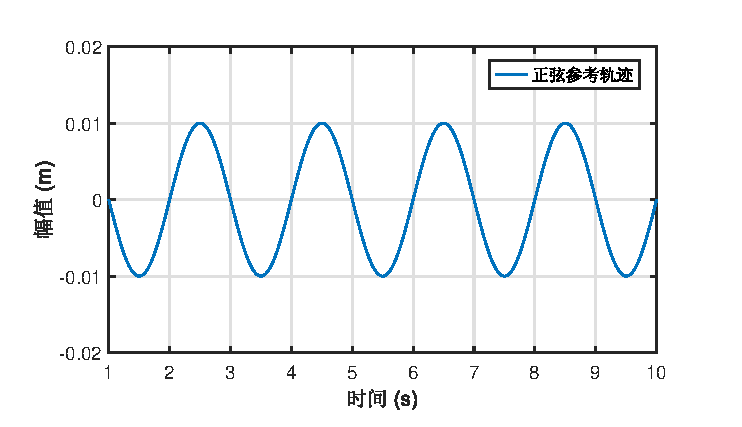
\includegraphics[width=12cm]{figures/正弦参考轨迹.eps}
%	\caption{正弦参考轨迹}
%	\label{正弦参考轨迹}
	\subfloat[0.5\,Hz]
	{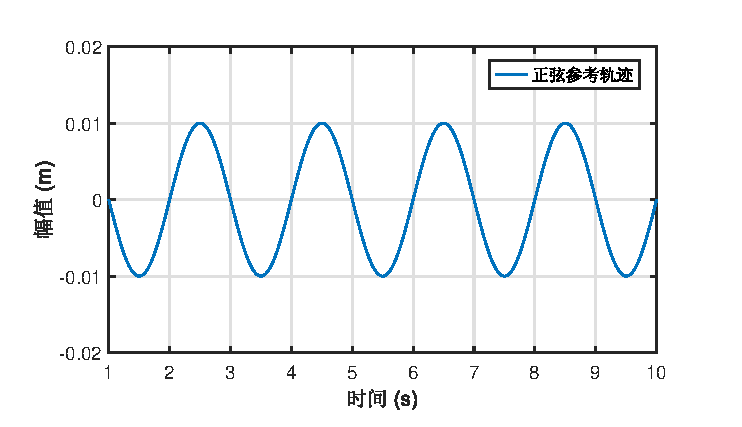
\includegraphics[width=12cm]{figures/正弦参考轨迹.eps}
		\label{Sin1} }\\
	\subfloat[1\,Hz]
	{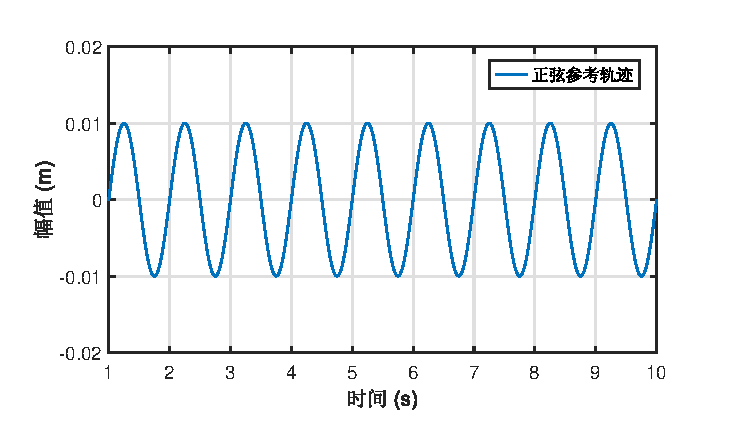
\includegraphics[width=12cm]{figures/正弦参考轨迹1.eps}
		\label{Sin2} }
	\caption{两组不同频率的正弦参考轨迹}
	\label{正弦参考轨迹}
\end{figure}
2)三组三阶轨迹,如图\ref{3组三阶轨迹}所示。具体参数为:

(a) 位移100$\,\text{mm}$,最大速度分别为100$\,\text{mm$/$s}$,最大加速度为4000$\,\text{mm/s$^2$}$;

(b) 位移100$\,\text{mm}$,最大速度分别为150$\,\text{mm$/$s}$,最大加速度为4000$\,\text{mm/s$^2$}$;

(c) 位移100$\,\text{mm}$,最大速度分别为200$\,\text{mm$/$s}$,最大加速度为4000$\,\text{mm/s$^2$}$。

这里为了使得实验结果更加充分,考虑了三种不同的实验设置情况,分别为:

\textbf{实验A.} 无负载情况下对名义模型进行实验测试;

\textbf{实验B.} 有$0.437\,\text{kg}$负载情况下测试对模型参数变化的鲁棒性;

\textbf{实验C.} 在稳态条件下在控制器输出加入$0.5\,\text{V}$持续时间$1\,\text{s}$的外部阶跃扰动(仅正弦输入情况下 5s$\sim$6s)。


\begin{figure}[H]
	\centering
%	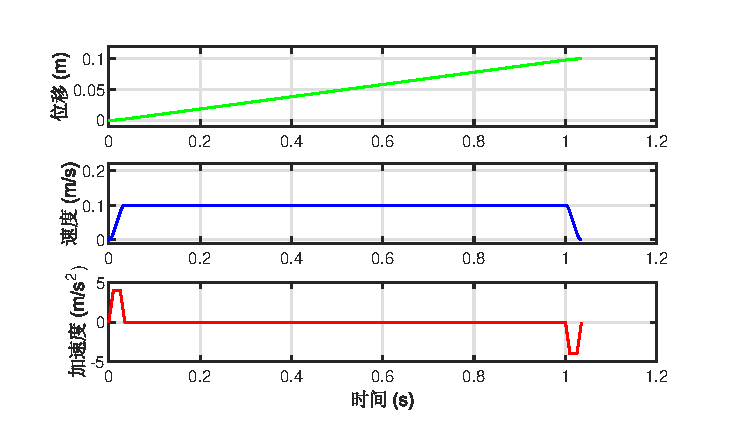
\includegraphics[width=12cm]{figures/三阶轨迹.eps}
%	\caption{三阶S轨迹}\\
    \subfloat[100$\,\text{mm/s}$]
	{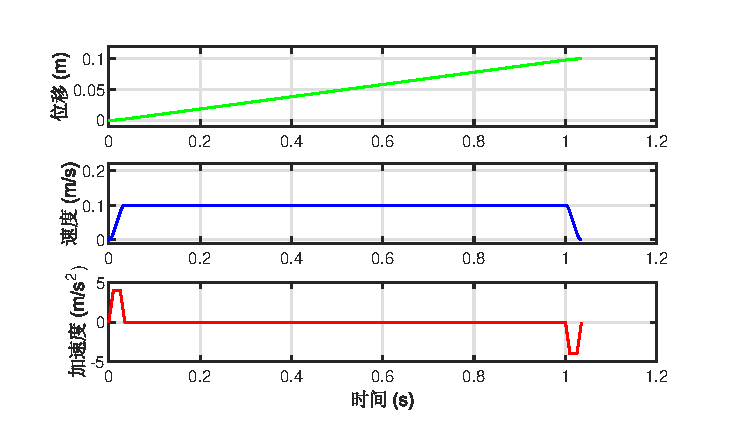
\includegraphics[width=12cm]{figures/三阶轨迹.eps}
		\label{S1} }\\
	\subfloat[150$\,\text{mm/s}$]
	{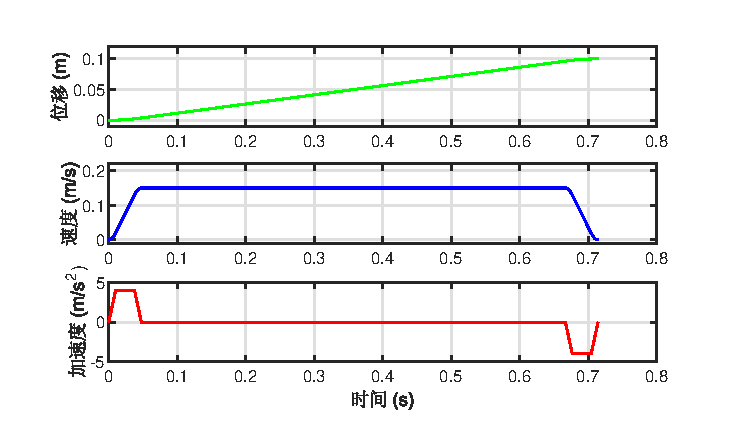
\includegraphics[width=12cm]{figures/三阶轨迹1.eps}
		\label{S2} }\\
	\subfloat[200$\,\text{mm/s}$]
	{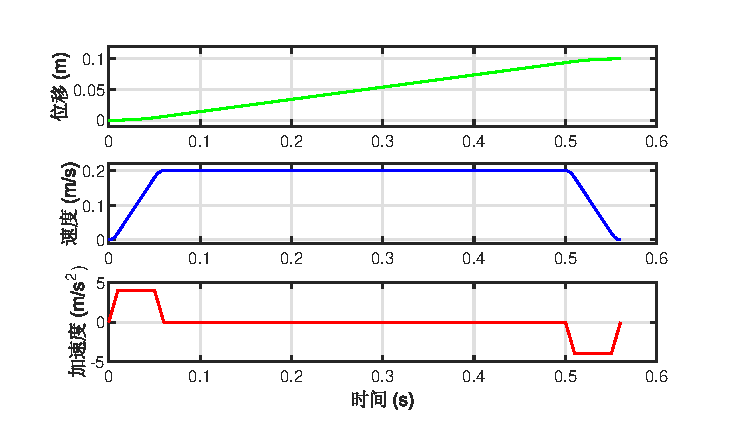
\includegraphics[width=12cm]{figures/三阶轨迹2.eps}
		\label{S3} }
	\caption{不同最大速度的三阶轨迹}
	\label{3组三阶轨迹}
\end{figure}
\section{实验结果与分析}
\subsection{性能评价指标}
为了能够量化地表征控制系统的位置跟踪性能和扰动抑制能力,实验结果的具体性能评价指标设定如下:
\begin{comment}
\begin{enumerate}
	\item 均方根误差(Root Mean Square Error, RMSE):
	\begin{equation}
	\text{RMSE}=\sqrt{\frac{1}{N}\sum_{i=1}^{N}|e(i)|^{2}}
	\end{equation}
	式中,$N$为观测位置跟踪数据的总个数。
	\item 最大绝对误差(Maximum Absolute Error, MAE):
	\begin{equation}
	\text{MAE}=\text{max}\left|e(i)\right|,\,i \in\{1, \ldots, N\}
	\end{equation}
	式中,$N$为观测位置跟踪数据的总个数。
	\item 平均绝对误差(Mean Absolute Deviation, MAD):
	\begin{equation}
	\text{MAD}=\frac{1}{N}\sum_{i=1}^{N}|e(i)|, i \in\{1, \ldots, N\}
	\end{equation}
	式中,$N$为观测位置跟踪数据的总个数。
	\item 移动平均值(Moving Average, MA):
	\begin{equation}
	\text{MA}(i)=\frac{1}{n_e} \sum_{j=i-n_e / 2}^{i+n_e / 2-1} e(j), i \in\{1, \ldots, N\}
	\end{equation}
	移动标准差(Moving Standard Deviation, MSD)\cite{butler2011position}。
	\\
	\begin{equation}
	\text{MSD}(i)=\sqrt{\frac{1}{n_e} \sum_{j=i-n_e / 2}^{i+n_e / 2-1}\left[e(j)-\text{MA}(i)\right]^{2}}, i \in\{1, \ldots, N\}
	\end{equation}
	式中,$n_e\in N^{+}$表示曝光时间窗内的数据个数,其值等于曝光时间除以系统采样时间;$N$为观测位置跟踪数据的总个数。MA和MSD在实际半导体装备中,常用作评价系统位置跟踪性能的指标。以光刻机为例,MA用来表征曝光期间的平均位置误差,代表位置跟踪误差的低频成分;MSD用来表征运动台的定位精度,代表位置跟踪误差的高频成分。因为光刻机系统的关键尺寸和套刻精度都与MA和MSD相关,因此,MA和MSD指标性能至关重要。本文的实验平台虽然不是基于光刻机,但是仍然可以用MA和MSD来作为评价指标对所提方法在精密直线运动平台上跟踪三阶轨迹的位置跟踪性能进行表征\cite{付雪微0有铁芯直线电机推力波动的分析与补偿方法研究}。
	\begin{comment}
	\item 位置误差的方差($S^2$):
	\begin{equation}
	S^{2}=\sum_{i=1}^{N}|e(i)-\bar{e}|^{2}, \forall i \in\{1, \ldots, N\}, \bar{e}=\frac{1}{N} \sum_{i=1}^{N} e(i), \forall i \in\{1, \ldots, N\}
	\end{equation}
	$S^2$表征了所观测的位置跟踪误差的平均波动情况。
\end{enumerate}
\end{comment}

	1. 均方根误差(Root Mean Square Error, RMSE):
	\begin{equation}
	\text{RMSE}=\sqrt{\frac{1}{N}\sum_{i=1}^{N}|e(i)|^{2}}
	\end{equation}
	式中,
	
	$N$为所观测位置跟踪误差数据的总个数。
	
	2. 最大绝对误差(Maximum Absolute Error, MAE):
	\begin{equation}
	\text{MAE}=\text{max}\left|e(i)\right|,\,i \in\{1, \ldots, N\}
	\end{equation}
	式中,
	
	$N$为所观测位置跟踪误差数据的总个数。
	
	3. 平均绝对误差(Mean Absolute Deviation, MAD):
	\begin{equation}
	\text{MAD}=\frac{1}{N}\sum_{i=1}^{N}|e(i)|, i \in\{1, \ldots, N\}
	\end{equation}
	式中,
	
	$N$为所观测位置跟踪误差数据的总个数。
	
	4. 移动平均值(Moving Average, MA),
	\begin{equation}
	\text{MA}(i)=\frac{1}{n_e} \sum_{j=i-n_e / 2}^{i+n_e / 2-1} e(j), i \in\{1, \ldots, N\}
	\end{equation}
	
	移动标准差(Moving Standard Deviation, MSD)\cite{butler2011position}。	(MA和MAS指标仅用于三阶轨迹位置跟踪实验)
	\begin{equation}
	\text{MSD}(i)=\sqrt{\frac{1}{n_e} \sum_{j=i-n_e / 2}^{i+n_e / 2-1}\left[e(j)-\text{MA}(i)\right]^{2}}, i \in\{1, \ldots, N\}
	\end{equation}
	式中,
	
	$n_e\in N^{+}$表示曝光时间窗内的数据个数,其值等于曝光时间除以系统采样时间;
	
	$N$为所观测位置跟踪误差数据的总个数。MA和MSD在实际半导体装备中,常用作评价系统位置跟踪性能的指标。以光刻机为例,MA用来表征曝光期间的平均位置误差,代表位置跟踪误差的低频成分;MSD用来表征运动台的定位精度,代表位置跟踪误差的高频成分。因为光刻机系统的关键尺寸和套刻精度都与MA和MSD相关,因此,MA和MSD指标性能至关重要。本文的实验平台虽然不是基于光刻机,但是仍然可以用MA和MSD来作为评价指标对所提方法在精密直线运动平台上跟踪三阶轨迹的位置跟踪性能
	进行表征\cite{付雪微0有铁芯直线电机推力波动的分析与补偿方法研究}。
\begin{comment}
	\item 位置误差的方差($S^2$):
	\begin{equation}
	S^{2}=\sum_{i=1}^{N}|e(i)-\bar{e}|^{2}, \forall i \in\{1, \ldots, N\}, \bar{e}=\frac{1}{N} \sum_{i=1}^{N} e(i), \forall i \in\{1, \ldots, N\}
	\end{equation}
	$S^2$表征了所观测的位置跟踪误差的平均波动情况。
}
\end{comment}
\subsection{递推最小二乘积分滑模控制器实验结果分析}
基于RLS的积分滑模控制方法的主要优势就是能够实现自适应逆模型前馈控制以及定位力扰动主要成分的自适应前馈补偿,同时积分滑模反馈控制保证了闭环系统的渐近稳定性。这里为了体现逆模型前馈的性能,选择三阶轨迹作为输入参考信号进行实验验证,实验分别在实验A和实验B情况下完成,主要在于对比改进前和改进后二者的瞬态性能和跟踪精度,下面详细介绍实验情况并进行结果分析。

%为了公平地比较本文所提的基于改进型递推最小二乘的积分滑模控制方法(Improved Recursive Least Square Integral Sliding Mode Control, IRLSISMC)

为了公平地比较IRLSISMC与TRLSISMC的性能,将二者共有的参数保持一致,通过调试优化,这里分别将二者的参数设置如下:

1. TRLSISMC:
\begin{equation}
\lambda=800,\,\eta=3,\,\beta=20
\end{equation}



2. IRLSISMC:
\begin{equation}
\lambda=800,\,\eta=3,\,\beta=20,\,\zeta=0.999
\end{equation}
下面具体介绍两种实验情况下,TRLSISMC和IRLSISMC方法的实验情况。

(1)实验A

实验A中,系统名义模型采用事先辨识好的等效质量$M_e=\text{0.12$\,$Vs$^{2}$/m}$,测试TRLSISMC与提出的IRLSISMC在名义模型下的位置跟踪性能,其中,输入的参考轨迹为不同最大速度的三阶轨迹,得到的位置跟踪误差曲线如图\ref{不同最大速度三阶S轨迹名义模型情况下位置跟踪误1}所示。



这种情况下,影响系统位置跟踪性能的主要因素是系统的定位力、摩擦力以及机械系统本身的模态。从位置跟踪误差曲线可以看到,在相同最大速度情况下,两种方法在加减速段的位置跟踪误差没有明显区别,这是因为加减速段主要发挥作用的仍然是逆模型前馈部分。而IRLSISMC方法匀速段的位置跟踪误差明显小于TRLSISMC方法匀速段的位置跟踪误差,这是因为匀速阶段粘滞摩擦力近似为定值,定位力扰动是其扰动的主要来源,而前者在其回归向量中引入了定位力基频成分的扰动形式,能够有效地对定位力扰动进行实时在线补偿。纵向分析不同速度之间,可以发现随着速度的增大,加速段的误差峰值有一定的增加,这主要是因为精密直线运动平台系统的粘滞摩擦与速度相关,高速情况下系统的粘滞摩擦力会更加明显,而且在加速阶段,系统往往需要更大的推力,因此会导致系统高速情况下加速阶段的位置跟踪误差较低速情况时更大一些。
\begin{figure}[H]\centering
	\subfloat[100$\,\text{mm/s}$]
	{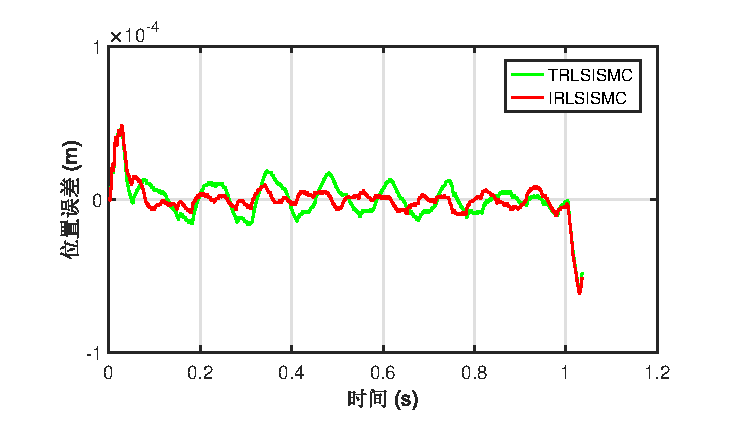
\includegraphics[width=12cm]{figures/rls100E.eps}
		\label{rls100mm} }\\
	\subfloat[150$\,\text{mm/s}$]
	{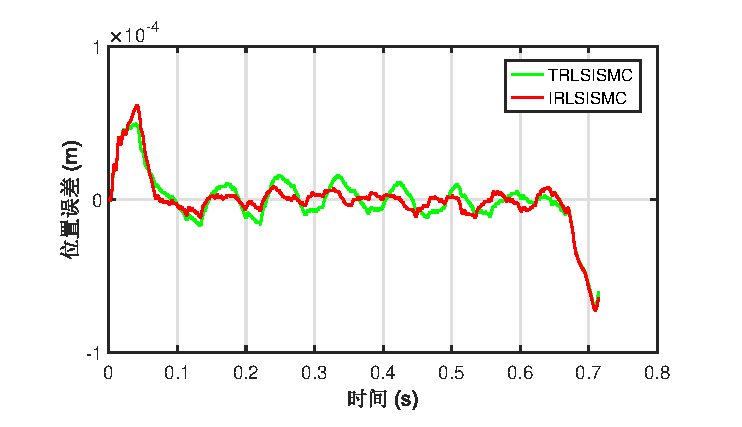
\includegraphics[width=12cm]{figures/rls150E.eps}
		\label{rls150mm} }\\
	\subfloat[200$\,\text{mm/s}$]
	{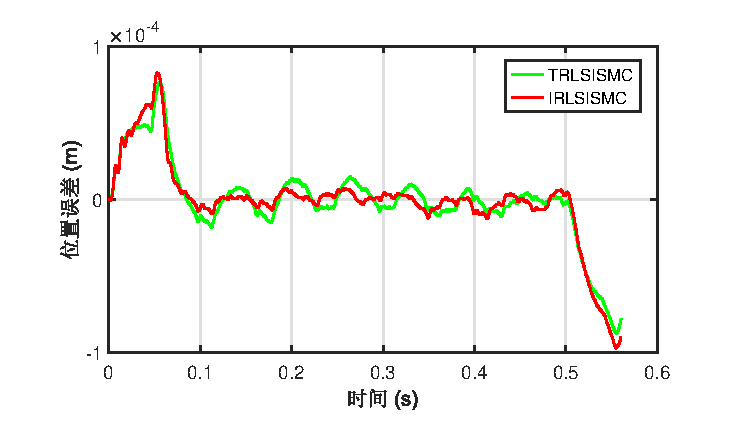
\includegraphics[width=12cm]{figures/rls200E.eps}
		\label{rls200mm} }
	\caption{不同最大速度三阶轨迹名义模型情况下位置跟踪误差}\label{不同最大速度三阶S轨迹名义模型情况下位置跟踪误1}
\end{figure}
为了进一步评价两种控制方法在精密直线运动平台上的控制性能,基于前面提到的性能评价指标对实验A中两种控制方法在匀速阶段的控制性能进行量化表征,具体的性能评价指标RMSE、MAE和MAD的结果如表\ref{实验A1}所示。需要说明的是,由于最大速度不同,因此三种速度情况下,用于计算性能评价指标的数据长度并不一致,具体为:1)100$\,\text{mm/s}$速度情况下,位置跟踪误差如图\ref{rls100mm}所示,选取0.1\,s$\sim$1\,s为所关心的数据段;2)150$\,\text{mm/s}$速度情况下,位置跟踪误差如图\ref{rls150mm}所示,选取0.1\,s$\sim$0.6\,s为所关心的数据段;3)200$\,\text{mm/s}$速度情况下,位置跟踪误差如图\ref{rls200mm}所示,选取0.1\,s$\sim$0.5\,s为所关心的数据段。
\begin{table}[H]
	\caption{实验A中不同最大速度三阶轨迹位置跟踪性能}
	\label{实验A1}
	\centering
	\setlength{\tabcolsep}{3mm} 
	\begin{tabular}{ccccc}
		\toprule[1.5pt]
		& \text{参考轨迹} & RMSE ($\text{$\upmu$m}$) & MAE ($\text{$\upmu$m}$) & $\text{MAD}$($\text{$\upmu$m}$)   \\ 
		\midrule
		\multirow{3}{*}{TRLSISMC}     
		%& C             & 9.57      & 41.4 &0  &0    \\
		& 100\,$\text{mm/s }$        & 8.37      & 18.6 &7.14   \\  
		& 150\,$\text{mm/s }$        & 8.27      & 16.8 &7.24     \\ 
		& 200\,$\text{mm/s }$        & 7.25      & 18.5 &6.06     \\
		\midrule
		\multirow{3}{*}{IRLSISMC} 
		& 100\,$\text{mm/s }$        & 4.28      & 10.8 &3.50  \\  
		& 150\,$\text{mm/s }$        & 4.43      & 11.7 &3.47     \\ 
		& 200\,$\text{mm/s }$        & 4.30      & 12.5 &3.37     \\
		\bottomrule[1.5pt]
	\end{tabular}
\end{table}

分析表格中的结果,可以发现,100\,$\text{mm/s}$三阶轨迹输入情况下,IRLSISMC方法的RMSE可以保持在4\,$\upmu$$\text{m}$附近,而TRLSISMC方法的MAE则在8\,$\upmu$$\text{m}$附近,说明前者的位置跟踪性能更加稳定,即位置跟踪误差的波动较小。IRLSISMC方法的MAE可以保持在11\,$\upmu$$\text{m}$附近,而TRLSISMC方法的MAE则在18\,$\upmu$$\text{m}$附近,说明IRLSISMC方法在匀速段的扰动抑制能力明显优于TRLSISMC方法,同时,MAD的结果也说明了IRLSISMC方法的位置跟踪误差整体较小。综合考虑不同速度下性能指标的变化情况,可以发现,随着速度的增加,两种控制方法的性能指标变化均不大,说明两种方法都比较能够适应速度变化的情况,不过IRLSISMC的位置跟踪精度和扰动抑制能力更好。

(2) 实验B

实验B中,在实验A的基础上添加了$0.437\,\text{kg}$负载,测试TRLSISMC与提出的IRLSISMC对系统模型参数变化的鲁棒性,得到的位置跟踪误差曲线如图\ref{不同最大速度三阶S轨迹有负载情况下位置跟踪误2}所示。定性分析,可以发现,当系统模型参数发生变化时,两种控制方法的位置跟踪性能仍然能够保持相对稳定的情况,与实验A中相比,可以清晰地看出,实验B中的位置跟踪误差曲线几乎维持在同一水平。

\begin{figure}[H]\centering
	\subfloat[100$\,\text{mm/s}$]
	{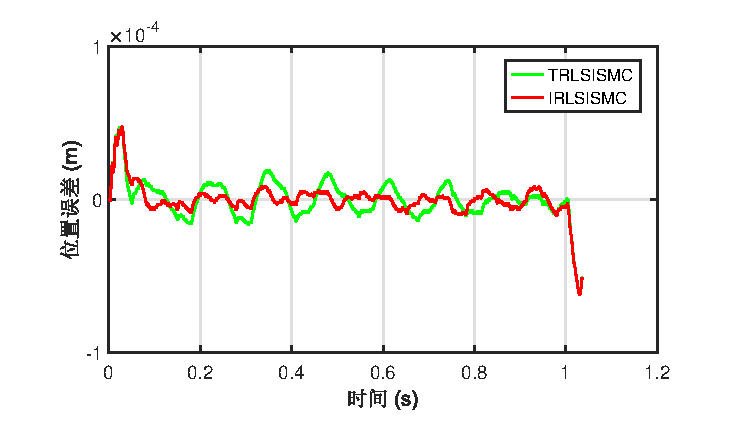
\includegraphics[width=12cm]{figures/rls100LoadE.eps}
		\label{rls100mmLoad} }\\
	\subfloat[150$\,\text{mm/s}$]
	{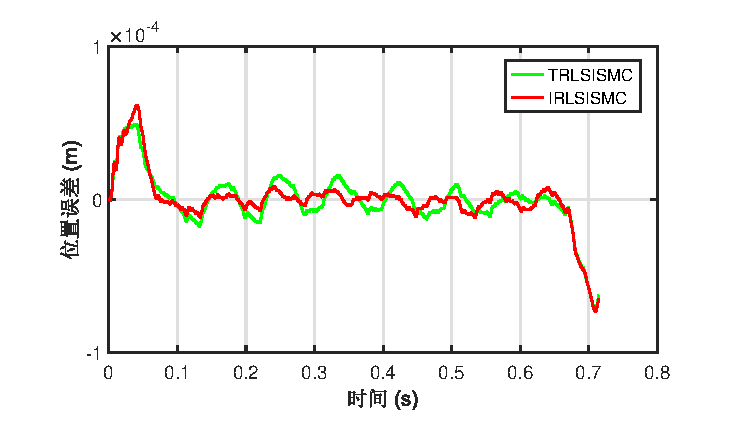
\includegraphics[width=12cm]{figures/rls150LoadE.eps}
		\label{rls150mmLoad} }\\
	\subfloat[200$\,\text{mm/s}$]
	{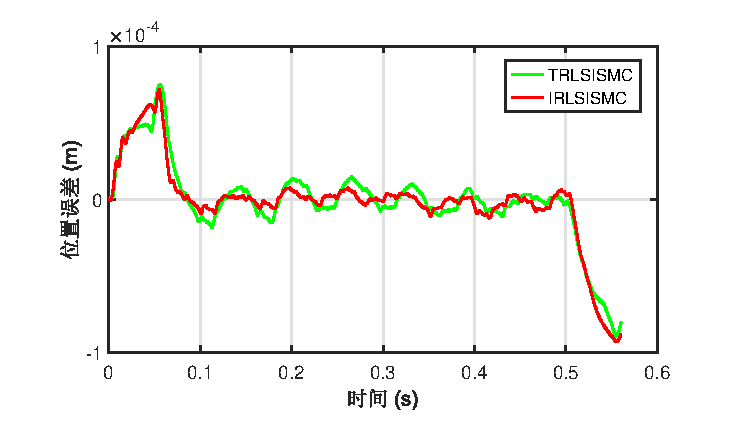
\includegraphics[width=12cm]{figures/rls200LoadE.eps}
		\label{rls200mmLoad} }
	\caption{不同最大速度三阶轨迹有负载情况下位置跟踪误差}\label{不同最大速度三阶S轨迹有负载情况下位置跟踪误2}
\end{figure}

为了更加清楚地认识两种控制方法对于系统模型参数变化的鲁棒性,还需要基于前面提到的性能指标对其位置跟踪误差曲线进行定量分析,
具体的性能评价指标与实验A中一致,结果如表\ref{实验B2}所示。
\begin{table}[H]
	\caption{实验B中不同最大速度三阶轨迹位置跟踪性能.}
	\label{实验B2}
	\centering
	\setlength{\tabcolsep}{3mm} 
	\begin{tabular}{ccccc}
		\toprule[1.5pt]
		& \text{参考轨迹} & RMSE ($\text{$\upmu$m}$) & MAE ($\text{$\upmu$m}$) & $\text{MAD}$($\text{$\upmu$m}$)   \\ 
		\midrule
		\multirow{3}{*}{TRLSISMC}     
		%& C             & 9.57      & 41.4 &0  &0    \\
		& 100\,$\text{mm/s }$        & 8.41      & 18.7 &7.15   \\  
		& 150\,$\text{mm/s }$        & 8.30      & 17.8 &7.25     \\ 
		& 200\,$\text{mm/s }$        & 7.27      & 18.5 &6.06     \\
		\midrule
		\multirow{3}{*}{IRLSISMC} 
		& 100\,$\text{mm/s }$       & 4.26      & 10.8 &3.50  \\  
		& 150\,$\text{mm/s }$       & 4.37      & 11.7 &3.45     \\ 
		& 200\,$\text{mm/s }$       & 4.32      & 12.2 &3.43     \\
		\bottomrule[1.5pt]
	\end{tabular}
\end{table}



分析表格中的结果,容易发现,与实验A对比,实验B中的性能指标与实验A中的性能指标相差并不大,这充分说明了两种方法均能够很好地应对系统模型参数的摄动,但IRLSISMC方法的位置跟踪性能仍然优于TRLSISMC。

对实验A和实验B中的三阶轨迹匀速段位置跟踪误差进行了MA和MSD分析,结果如图\ref{不同速度情况下位置跟踪误差MA、MSD曲线2}所示。可以清楚地看到,当运行速度提高时,TRLSISMC方法的MA和MSD均有不同程度的增大,而IRLSISMC方法的MA和MSD都是稳定地维持在较低水平,这充分说明了IRLSISMC方法的位置跟踪性能优于TRLSISMC方法,位置跟踪精度以及位置跟踪误差的稳定性都有很大的提升。

从具体的数值角度来分析,在最大速度为100\,$\text{mm/s}$且无负载情况时,TRLSISMC方法匀速段跟踪误差的MA最大为8.93\,$\text{$\upmu$m}$,MSD最大为13.4\,$\text{$\upmu$m}$,而所提的IRLSISMC方法匀速段跟踪误差的MA最大为3.99\,$\text{$\upmu$m}$,MSD最大为6.27\,$\text{$\upmu$m}$,与TRLSISMC方法相比,IRLSISMC方法的位置跟踪性能得到了极大的提升。在有负载的情况下,MA和MSD的值也几乎保持一致,IRLSISMC方法的MA和MSD分别为4.00\,$\text{$\upmu$m}$和6.23\,$\text{$\upmu$m}$,这一结果从位置跟踪误差的整体性能层面也验证了所提IRLSISMC方法能够有效地提高系统位置跟踪精度,并对系统模型参数变化有一定的鲁棒性。

在最大速度为200\,$\text{mm/s}$且无负载情况时,TRLSISMC方法匀速段跟踪误差的MA最大为8.11\,$\text{$\upmu$m}$,MSD最大为10.7\,$\text{$\upmu$m}$,而所提的IRLSISMC方法匀速段跟踪误差的MA最大为6.31\,$\text{$\upmu$m}$,MSD最大为5.13\,$\text{$\upmu$m}$。纵向对比不同速度情况下匀速段跟踪误差的MA和MSD的变化,可以发现系统运行速度从100\,$\text{mm/s}$到200\,$\text{mm/s}$时,系统的MA和MSD并不是都随着速度的提高而增大的,这主要是因为实验所用精密直线运动平台的摩擦力中包含的Stribeck效应导致系统在高速运行情况下,如第二章公式(\ref{2.11})表示的摩擦力模型所示,摩擦力的非线性特性会相对降低,但是粘滞摩擦力的值仍然是较低速情况下更大一些,这才导致了高速情况下系统的MA会有所增加,而MSD反而会有一定程度的降低,说明这时位置跟踪误差虽然值有所增加,但是却更加均匀,离散程度更小。

\begin{figure}[H]
	\centering
	\subfloat[100$\,\text{mm/s}$三阶S轨迹无负载]{\label{rlsMAMSD100mm无负载}%%
		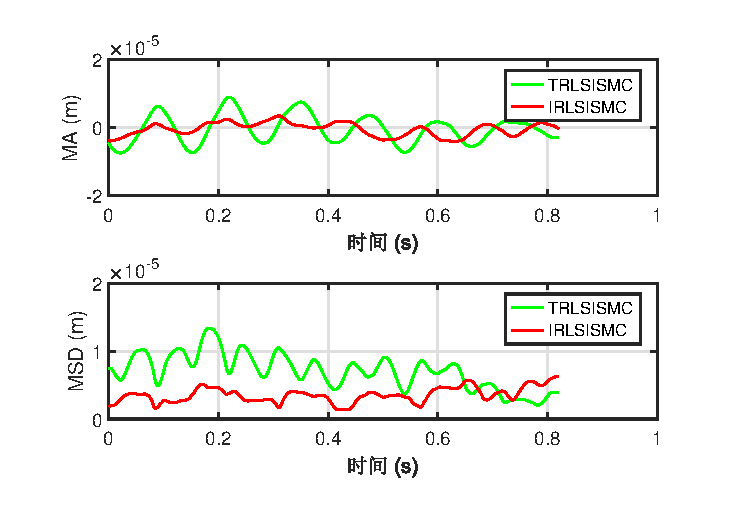
\includegraphics[width=7.6cm]{figures/rlsMAMSD100mm无负载.eps}} 	
	\subfloat[100$\,\text{mm/s}$三阶S轨迹有负载]{\label{rlsMAMSD100mm有负载}%%
		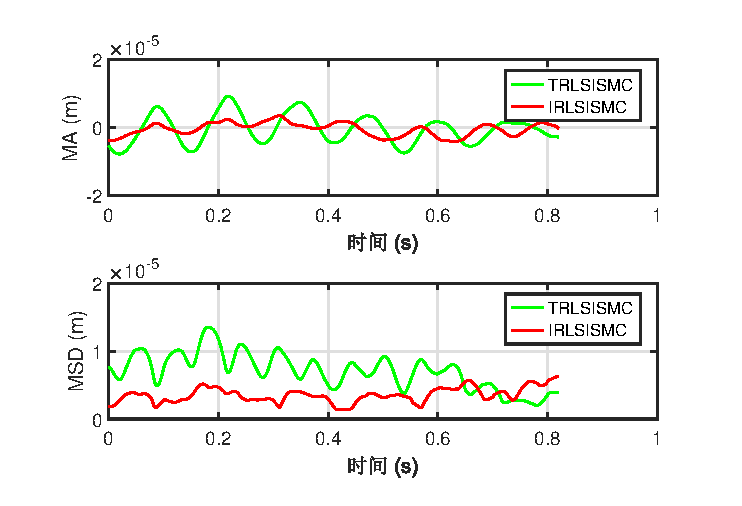
\includegraphics[width=7.6cm]{figures/rlsMAMSD100mm有负载.eps}} \\
	\subfloat[150$\,\text{mm/s}$三阶S轨迹无负载]{\label{rlsMAMSD150mm无负载}%%
		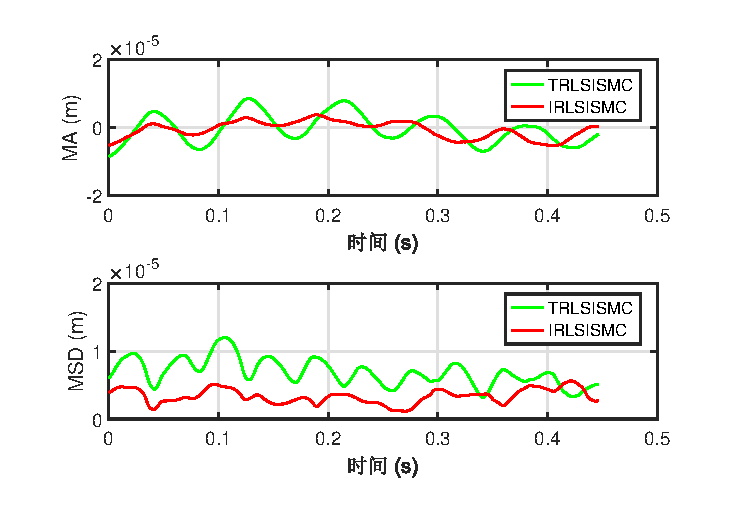
\includegraphics[width=7.6cm]{figures/rlsMAMSD150mm无负载.eps}} 	
	\subfloat[150$\,\text{mm/s}$三阶S轨迹有负载]{\label{rlsMAMSD150mm有负载}%%
		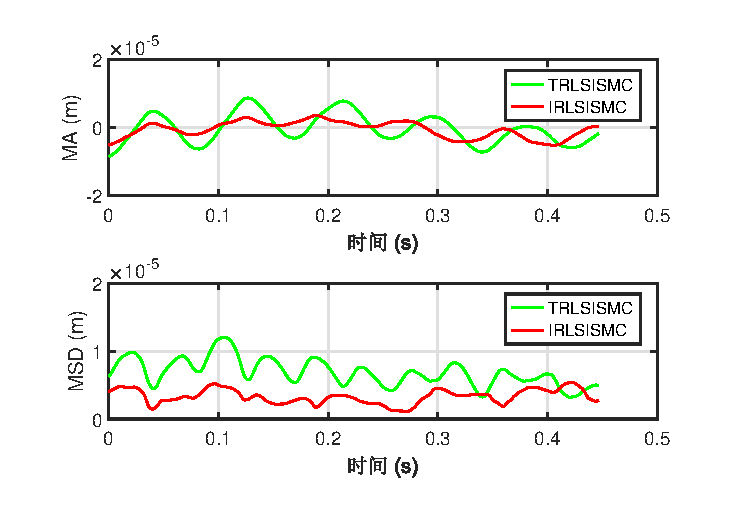
\includegraphics[width=7.6cm]{figures/rlsMAMSD150mm有负载.eps}} \\
	\subfloat[200$\,\text{mm/s}$三阶S轨迹无负载]{\label{rlsMAMSD200mm无负载}%%
		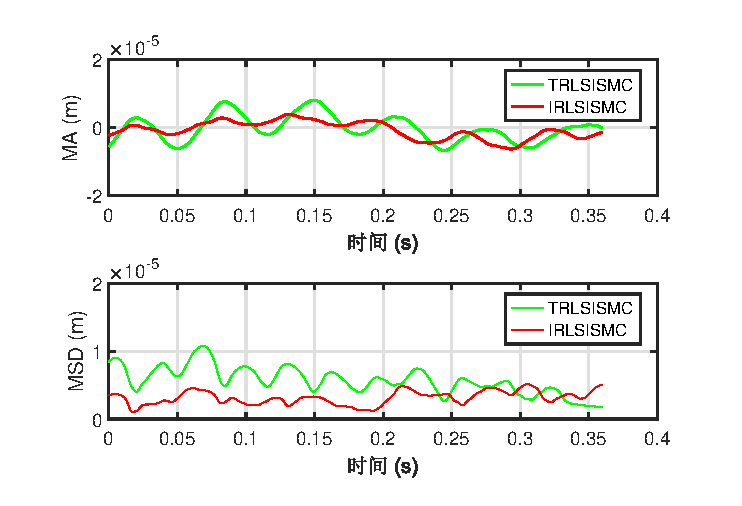
\includegraphics[width=7.6cm]{figures/rlsMAMSD200mm无负载.eps}} 	
	\subfloat[200$\,\text{mm/s}$三阶S轨迹有负载]{\label{rlsMAMSD200mm有负载}%%
		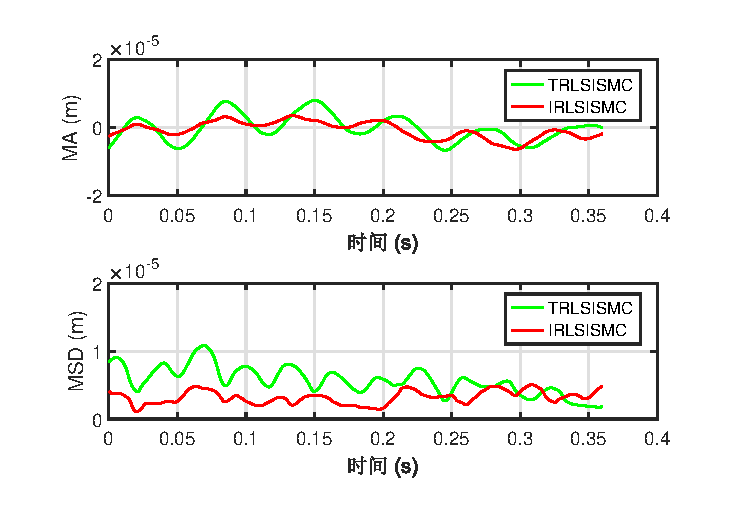
\includegraphics[width=7.6cm]{figures/rlsMAMSD200mm有负载.eps}} \\
	\caption{不同速度情况下位置跟踪误差MA、MSD曲线}
	\label{不同速度情况下位置跟踪误差MA、MSD曲线2}
\end{figure}





\subsection{多核神经网络动态边界层滑模控制器实验结果分析}
多核神经网络动态边界层滑模控制方法的提出主要是为了提高精密直线运动平台的位置跟踪性能和扰动抑制能力,这里为了更有力地表明所提方法的有效性以及设计参数对于整个控制系统性能的影响,在两种参考轨迹的输入情况下分别就三种实验情况都与传统RBF神经网络滑模控制进行了对比实验,下面详细介绍实验情况并进行结果分析。

为了公平地比较所提出的多核神经网络动态边界层滑模控制方法(Multi-Kernel Neural Network Sliding Mode Control, MNNSMC)与传统RBF神经网络自适应滑模控制方法(Adaptive Sliding Mode Control, ASMC),将二者共同的参数设置一致,只保留所提出的方法的特有的参数设置可调。通过调试优化,这里分别将二者的参数设置如下:
\begin{enumerate}
	\item 传统ASMC:
	\begin{equation}
	\lambda =800\text{,}\,\eta =3\text{,}\,\gamma =2\cdot\text{exp}(-4)\text{,}\,\Delta =0.005
	\end{equation}
	\item MNNSMC:
	\begin{equation}
	\begin{aligned}
	&\lambda=800\text{,}\,\eta =3\text{,}\,{{\Delta}_{0}}=0.005\text{,}\,\alpha=3\text{,} \\ 
	&\textbf{ }\!\!{\gamma}=\text{diag}([\underbrace{2\text{,}\cdots\text{,}\,2}_{N_h}\text{,}\underbrace{1\text{,}\cdots\text{,}\,1}_{2N_t}\text{,}\,0.5]\cdot\exp(-4)) \\ 
	\end{aligned}
	\end{equation}
	式中, $N_h$\,=\,$5$,即高斯核函数的节点有5个;$N_t$\,=\,$4$,即三角核函数的节点有4对,分别对应4个定位力主要频率;Sigmoid核函数的节点只有1个。
\end{enumerate}

三种实验设置下,对本文所提出的MNNSMC方法与传统ASMC方法在精密直线运动平台上的控制性能进行了验证,下面介绍具体的实验情况。

(1) 实验A

实验A中,系统名义模型仍采用事先辨识好的等效质量$M_e=\text{0.12$\,$Vs$^{2}$/m}$,测试传统ASMC与提出的MNNSMC在名义模型下的位置跟踪性能,不同频率的正弦参考轨迹与不同最大速度的三阶轨迹作为位置参考输入信号,得到的位置跟踪误差曲线如图\ref{不同频率正弦参考轨迹名义模型情况下位置跟踪误差}和图\ref{不同最大速度三阶S轨迹名义模型情况下位置跟踪误}所示。
如前面提到的,实验A的设置下,影响系统位置跟踪性能的主要因素是系统的定位力、摩擦力以及机械系统本身的模态。

当输入正弦变化的位置参考轨迹时,得到的位置跟踪误差曲线如图\ref{不同频率正弦参考轨迹名义模型情况下位置跟踪误差}所示,可以发现,本文提出的MNNSMC方法的位置跟踪误差明显小于ASMC方法,而且对比两种不同频率的正弦信号时能够发现,正弦信号的频率越高,即参考轨迹的速度、加速度越大时,MNNSMC方法的优势体现的越明显,这是因为MNNSMC方法中引入了精密直线运动平台的定位力和摩擦力模型,这种多核神经网络模型能够更有效地适应高速高精度运行要求。可以看到,在正弦频率较高的时,MNNSMC方法的暂态和ASMC相当,但是稳态性能远远优于ASMC方法,这是因为神经网络权重的调节都需要一定的时间,这在实际工程应用对于整定时间要求不太严苛时,是完全可以接受的。


\begin{figure}[H]\centering
	\subfloat[0.5$\,\text{Hz}$]
	{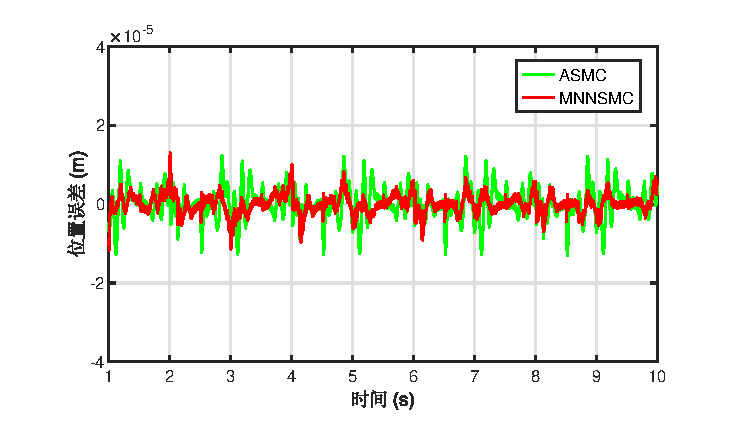
\includegraphics[width=12cm]{figures/正弦05Hz无负载.eps}
		\label{正弦05无负载} }\\
	\subfloat[1$\,\text{Hz}$]
	{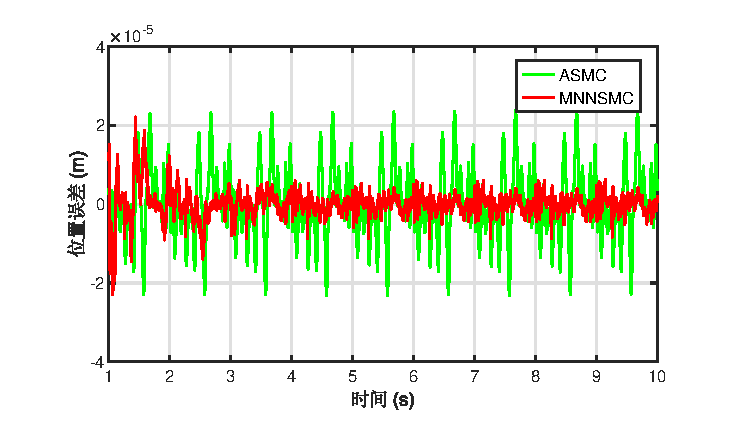
\includegraphics[width=12cm]{figures/正弦1Hz无负载.eps}
		\label{正弦1Hz无负载} }
	\caption{不同频率正弦参考轨迹名义模型情况下位置跟踪误差}\label{不同频率正弦参考轨迹名义模型情况下位置跟踪误差}
\end{figure}
当系统输入不同最大速度的三阶轨迹时,系统位置跟踪误差如图\ref{不同最大速度三阶S轨迹名义模型情况下位置跟踪误}所示,可以发现,本文提出的MNNSMC方法较传统的ASMC方法在加减速段和匀速段的位置跟踪性能方面都有明显的提升。而且随着速度的增加,MNNSMC方法比ASMC方法能够更好地适应高速的情况。仔细对比不同速度情况下的位置跟踪误差曲线,不难发现,MNNSMC方法在加速阶段的位置跟踪误差曲线的峰值有一定的增加,但是仍远小于传统ASMC方法。在匀速阶段,传统ASMC的误差随着速度的增加而增加的较为明显,提出的MNNSMC方法的位置跟踪误差则有减小的趋势,这是因为MNNSMC中提出的动态边界层与速度相关,能够较好地适应高速的情况,而神经网络补偿部分则能够更好地抑制系统内部和外部的总扰动,从而能够提高高速运行情况下的位置跟踪精度和扰动抑制能力。
\\
\begin{figure}[H]\centering
	\subfloat[100$\,\text{mm$/$s}$]
	{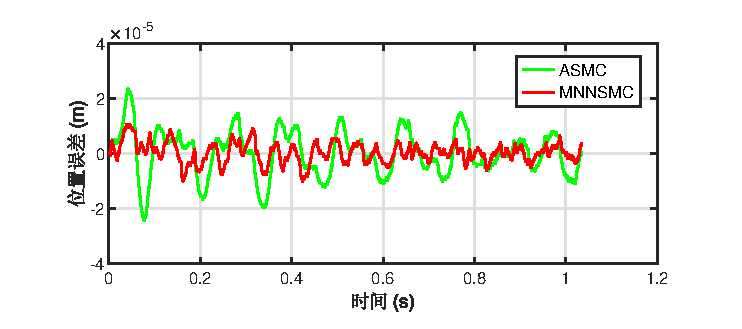
\includegraphics[width=12cm]{figures/S轨迹100无负载.eps}
		\label{S轨迹100无负载} }\\
	\subfloat[150$\,\text{mm$/$s}$]
	{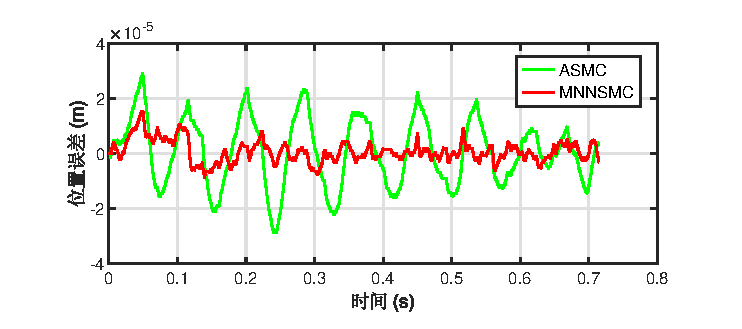
\includegraphics[width=12cm,height=5cm]{figures/S轨迹150无负载.eps}
		\label{S轨迹150无负载} }\\
	\subfloat[200$\,\text{mm$/$s}$]
	{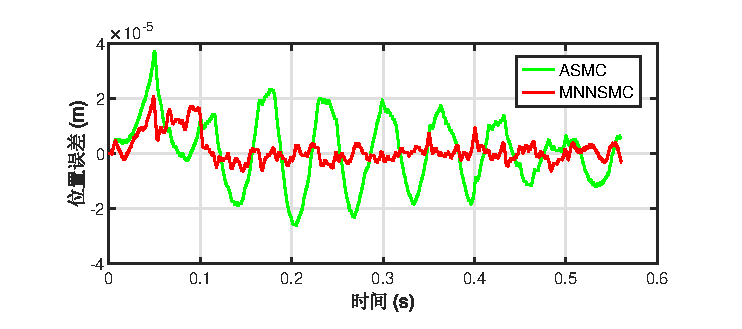
\includegraphics[width=12cm]{figures/S轨迹200无负载.eps}
		\label{S轨迹200无负载} }
	\caption{不同最大速度三阶轨迹名义模型情况下位置跟踪误}\label{不同最大速度三阶S轨迹名义模型情况下位置跟踪误}
\end{figure}

\begin{comment}
\begin{figure}[H]
	\centering
	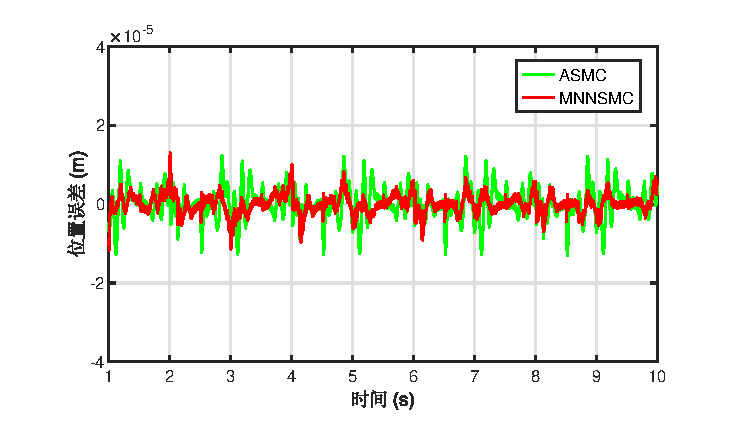
\includegraphics[width=12cm]{figures/正弦05Hz无负载.eps}
	\caption{0.5$\,\text{Hz}$正弦参考轨迹名义模型情况下位置跟踪误差}
	\label{正弦05无负载}
\end{figure}
\begin{figure}[H]
	\centering
	\includegraphics[width=12cm]{figures/正弦1Hz无负载.eps}
	\caption{1$\,\text{Hz}$正弦参考轨迹名义模型情况下位置跟踪误差}
	\label{正弦1Hz无负载}
\end{figure}
\end{comment}



\begin{comment}
\begin{figure}[H]
	\centering
	\includegraphics[width=12cm]{figures/S轨迹100无负载.eps}
	\caption{最大速度为100$\,\text{mm$/$s}$的三阶S轨迹名义模型情况下位置跟踪误差}
	\label{S轨迹100无负载}
\end{figure}
\begin{figure}[H]
	\centering
	\includegraphics[width=12cm]{figures/S轨迹150无负载.eps}
	\caption{最大速度为150$\,\text{mm$/$s}$的三阶S轨迹名义模型情况下位置跟踪误差}
	\label{S轨迹150无负载}
\end{figure}
\begin{figure}[H]
	\centering
	\includegraphics[width=12cm]{figures/S轨迹200无负载.eps}
	\caption{最大速度为200$\,\text{mm$/$s}$的三阶S轨迹名义模型情况下位置跟踪误差}
	\label{S轨迹200无负载}
\end{figure}
\end{comment}


为了进一步评价两种基于神经网络的控制方法在精密直线运动平台上的控制性能,这里对实验A中两种控制方法在匀速阶段的控制性能进行量化表征,具体的性能评价指标RMSE、MAE和MAD的结果如表\ref{实验A}所示。需要说明的是,当系统输入三阶轨迹时,由于最大速度不同,用于计算性能评价指标的数据长度并不一致,具体为:1)100$\,\text{mm/s}$速度情况下,位置跟踪误差如图\ref{S轨迹100无负载}所示,选取0.2\,s$\sim$1\,s为所关心的数据段;2)150$\,\text{mm/s}$速度情况下,位置跟踪误差如图\ref{S轨迹150无负载}所示,选取0.2\,s$\sim$0.6\,s为所关心的数据段;3)200$\,\text{mm/s}$速度情况下,位置跟踪误差如图\ref{S轨迹200无负载}所示,选取0.2\,s$\sim$0.5\,s为所关心的数据段。
\begin{table}[H]
	\caption{实验A中不同参考轨迹位置跟踪性能.}
	\label{实验A}
	\centering
	\setlength{\tabcolsep}{3mm} 
	\begin{tabular}{ccccc}
		\toprule[1.5pt]
		& \text{参考轨迹} & RMSE ($\text{$\upmu$m}$) & MAE ($\text{$\upmu$m}$) & $\text{MAD}$($\text{$\upmu$m}$)   \\ 
		\midrule
		\multirow{5}{*}{ASMC}     
		& 0.5Hz         & 4.08      & 13.1 &2.97     \\ 
		& 1Hz           & 8.94      & 23.6 &6.70     \\ 
		%& C             & 9.57      & 41.4 &0  &0    \\
		& 100\,$\text{mm/s }$            & 7.55      & 19.5 &6.13   \\  
		& 150\,$\text{mm/s }$             & 13.1      & 28.6 &11.3     \\ 
		& 200\,$\text{mm/s }$             & 12.2      & 26.0 &10.4     \\
		\midrule
		\multirow{5}{*}{MNNSMC} 
		& 0.5Hz           & 2.37      & 13.1 &1.73    \\ 
		& 1Hz             & 3.47      & 23.0 &2.19     \\ 
		& 100\,$\text{mm/s }$            & 3.31      & 10.1 &2.63  \\  
		& 150\,$\text{mm/s }$             & 2.73      & 9.23 &2.10     \\ 
		& 200\,$\text{mm/s }$             & 2.38      & 9.40 &1.87    \\
		\bottomrule[1.5pt]
	\end{tabular}
\end{table}

分析表格中的结果,可以发现,正弦信号输入情况下,频率为0.5\,Hz时,ASMC与MNNSMC的MAE都为13.1\,$\upmu$$\text{m}$,RMSE和MAD也都相差不大,但是当频率为1Hz时,虽然两种方法MAE的值仍然相差不大,但是MNNSMC方法的RMSE和MAD都小于ASMC方法的一半。这主要是因为当正弦信号频率变高,即参考轨迹的速度变快,扰动带来的影响也会更加明显,主要是粘滞摩擦力近似与速度成正比,而基于传统RBF的ASMC扰动补偿的能力有限,所提出的MNNSMC方法因为在核函数的设计中考虑了摩擦力的模型,因此MNN神经网络的收敛速度会更快,扰动补偿能力也会因此而显著提高。

最大速度为100\,$\text{mm/s}$的三阶轨迹输入情况下,MNNSMC方法的MAE可以保持在10\,$\upmu$$\text{m}$附近,而ASMC方法的MAE则在20\,$\upmu$$\text{m}$附近。前者的RMSE和MAD的值远远低于后者,这充分表明了本文所提MNNSMC方法在提高精密直线运动平台位置跟踪性能方面优于传统ASMC方法。此外,纵向对比不同速度情况下的位置跟踪性能,可以发现,随着速度的增加,ASMC位置跟踪性能的三项评价指标均有一定的恶化,但是MNNSMC方法的各项性能指标则相对较为稳定,这进一步表明MNNSMC的控制性能更优。

(2) 实验B

实验B中,在实验A的基础上添加了$0.437\,\text{kg}$负载,测试传统ASMC与提出的MNNSMC对系统模型参数变化的鲁棒性,得到的位置跟踪误差曲线如图\ref{不同频率正弦参考轨迹有负载情况下位置跟踪误差}和图\ref{不同最大速度三阶S轨迹有负载情况下位置跟踪误}所示。

当不同频率的正弦参考轨迹输入时,得到的系统位置跟踪误差曲线如图\ref{不同频率正弦参考轨迹有负载情况下位置跟踪误差}所示,与实验A相比,可以直观地看到,实验B的位置跟踪误差曲线没有明显的变化,这充分说明了两种基于神经网络的控制方法对于均能够很好地应对系统模型参数摄动,即鲁棒性好。

\begin{figure}[H]\centering
	\subfloat[0.5$\,\text{Hz}$]
	{\includegraphics[width=12cm]{figures/正弦05Hz有负载.eps}
		\label{正弦05有负载} }\\
	\subfloat[1$\,\text{Hz}$]
	{\includegraphics[width=12cm]{figures/正弦1Hz有负载.eps}
		\label{正弦1Hz有负载} }
	\caption{不同频率正弦参考轨迹有负载情况下位置跟踪误差}\label{不同频率正弦参考轨迹有负载情况下位置跟踪误差}
\end{figure}
当不同最大速度的三阶轨迹输入时,得到的系统位置跟踪误差曲线如图\ref{不同最大速度三阶S轨迹有负载情况下位置跟踪误}所示,仔细观察可以发现,与实验A相比,实验B中传统ASMC方法在加速阶段的位置跟踪误差峰值有略微的增加,这是因为加速阶段需要的推力有略微的增加,而本文提出的MNNSMC方法在加速阶段的位置跟踪误差则没有明显的变化。此外,在匀速阶段,两种方法的位置跟踪误差曲线均无明显变化,这同样说明了所提方法对于系统模型参数摄动具有较好的鲁棒性。


\begin{figure}[H]\centering
	\subfloat[100$\,\text{mm$/$s}$]
	{\includegraphics[width=12cm]{figures/S轨迹100有负载.eps}
		\label{S轨迹100有负载} }\\
	\subfloat[150$\,\text{mm$/$s}$]
	{\includegraphics[width=12cm]{figures/S轨迹150有负载.eps}
		\label{S轨迹150有负载} }\\
	\subfloat[200$\,\text{mm$/$s}$]
	{\includegraphics[width=12cm]{figures/S轨迹200有负载.eps}
		\label{S轨迹200有负载} }
	\caption{不同最大速度三阶轨迹有负载情况下位置跟踪误}\label{不同最大速度三阶S轨迹有负载情况下位置跟踪误}
\end{figure}
为了更具体地表征实验B中精密直线运动平台的位置跟踪性能,将定量分析的性能指标数据总结在表\ref{不同最大速度三阶S轨迹有负载情况下位置跟踪误}中,关心的数据段与实验A中一致:1)100$\,\text{mm/s}$速度情况下,位置跟踪误差如图\ref{S轨迹100无负载}所示,选取0.2\,s$\sim$1\,s为所关心的数据段;2)150$\,\text{mm/s}$速度情况下,位置跟踪误差如图\ref{S轨迹150无负载}所示,选取0.2\,s$\sim$0.6\,s为所关心的数据段;3)200$\,\text{mm/s}$速度情况下,位置跟踪误差如图\ref{S轨迹200无负载}所示,选取0.2\,s$\sim$0.5\,s为所关心的数据段。
\begin{comment}
\begin{figure}[H]
	\centering
	\includegraphics[width=12cm]{figures/正弦05Hz有负载.eps}
	\caption{0.5$\,\text{Hz}$正弦参考轨迹有负载情况下位置跟踪误差}
	\label{正弦05有负载}
\end{figure}
\begin{figure}[H]
	\centering
	\includegraphics[width=12cm]{figures/正弦1Hz有负载.eps}
	\caption{1$\,\text{Hz}$正弦参考轨迹有负载情况下位置跟踪误差}
	\label{正弦1Hz有负载}
\end{figure}
\begin{figure}[H]
	\centering
	\includegraphics[width=12cm]{figures/S轨迹100有负载.eps}
	\caption{最大速度为100$\,\text{mm$/$s}$的三阶S轨迹有负载情况下位置跟踪误差}
	\label{S轨迹100有负载}
\end{figure}
\begin{figure}[H]
	\centering
	\includegraphics[width=12cm]{figures/S轨迹150有负载.eps}
	\caption{最大速度为150$\,\text{mm$/$s}$的三阶S轨迹有负载情况下位置跟踪误差}
	\label{S轨迹150有负载}
\end{figure}
\begin{figure}[H]
	\centering
	\includegraphics[width=12cm]{figures/S轨迹200有负载.eps}
	\caption{最大速度为200$\,\text{mm$/$s}$的三阶S轨迹有负载情况下位置跟踪误差}
	\label{S轨迹200有负载}
\end{figure}
\end{comment}

\begin{table}[H]
	\caption{实验B中不同参考轨迹位置跟踪性能.}
	\label{实验B}
	\centering
	\setlength{\tabcolsep}{3mm} 
	\begin{tabular}{ccccc}
		\toprule[1.5pt]
		& \text{参考轨迹} & RMSE ($\text{$\upmu$m}$) & MAE ($\text{$\upmu$m}$) & $\text{MAD}$($\text{$\upmu$m}$)   \\ 
		\midrule
		\multirow{5}{*}{ASMC}     
		& 0.5Hz           & 4.13      & 14.2 &3.00   \\ 
		& 1Hz             & 9.06      & 23.2 &6.89   \\ 
		%& C             & 9.57      & 41.4 &0  &0    \\
		& 100\,$\text{mm/s }$            & 7.53      & 19.5 &6.12   \\  
		& 150\,$\text{mm/s }$             & 13.2      & 29.6 &11.5    \\ 
		& 200\,$\text{mm/s }$             & 12.3      & 26.0 &10.5     \\
		\midrule
		\multirow{5}{*}{MNNSMC} 
		& 0.5Hz           & 2.44      & 13.8 &1.77    \\ 
		& 1Hz             & 3.86      & 27.4 &2.31    \\ 
		& 100\,$\text{mm/s }$            & 3.39      & 10.2 &2.70  \\  
		& 150\,$\text{mm/s }$             & 2.82      & 9.20 &2.16     \\ 
		& 200\,$\text{mm/s }$             & 2.41      & 9.40 &1.90     \\
		\bottomrule[1.5pt]
	\end{tabular}
\end{table}

分析表格中的结果,与实验A对比,容易发现,实验B中的各项性能指标与实验A中的各项性能指标仍然保持在同一水平,这充分说明了两种基于神经网络的控制方法对于均能够很好地应对系统模型参数摄动问题,但MNNSMC方法的位置跟踪性能仍然优于ASMC。

对实验A和实验B中不同最大速度的三阶轨迹位置跟踪误差进行了MA和MSD分析,结果如图\ref{不同速度情况下位置跟踪误差MA、MSD曲线}所示。可以清楚地看到,当运行速度提高时,ASMC方法的MA和MSD均有不同程度的增大,而MNNSMC方法的MA和MSD都是稳定地维持在较低水平,这充分说明了MNNSMC方法的位置跟踪性能优于ASMC方法,平均位置误差和定位精度都有很大的提升。

从具体的数值角度来分析,在最大速度为100\,$\text{mm/s}$且无负载情况时,ASMC方法匀速段跟踪误差的MA最大为5.83\,$\text{$\upmu$m}$,MSD最大为11.9\,$\text{$\upmu$m}$,而所提的MNNSMC方法匀速段跟踪误差的MA最大为2.69\,$\text{$\upmu$m}$,MSD最大为4.95\,$\text{$\upmu$m}$,与ASMC方法相比,MNNSMC方法的位置跟踪性能得到了极大的提升。在有负载的情况下,MA和MSD的值也几乎保持一致,MNNSMC方法的MA和MSD分别为2.71\,$\text{$\upmu$m}$和5.07\,$\text{$\upmu$m}$,这一结果从位置跟踪误差的整体性能层面也验证了所提IRLSISMC方法能够有效地提高系统位置跟踪精度,并对系统模型参数摄动有一定的鲁棒性。


\begin{figure}[!t]
	\centering
	\subfloat[100$\,\text{mm/s}$三阶S轨迹无负载]{\label{100mm无负载}%%
		\includegraphics[width=7.5cm]{figures/100mm无负载.eps}} 	
	\subfloat[100$\,\text{mm/s}$三阶S轨迹有负载]{\label{100mm有负载}%%
		\includegraphics[width=7.5cm]{figures/100mm有负载.eps}} \\
	\subfloat[150$\,\text{mm/s}$三阶S轨迹无负载]{\label{150mm无负载}%%
		\includegraphics[width=7.5cm]{figures/150mm无负载.eps}} 	
	\subfloat[150$\,\text{mm/s}$三阶S轨迹有负载]{\label{150mm有负载}%%
		\includegraphics[width=7.5cm]{figures/150mm有负载.eps}} \\
	\subfloat[200$\,\text{mm/s}$三阶S轨迹无负载]{\label{200mm无负载}%%
		\includegraphics[width=7.5cm]{figures/200mm无负载.eps}} 	
	\subfloat[200$\,\text{mm/s}$三阶S轨迹有负载]{\label{200mm有负载}%%
		\includegraphics[width=7.5cm]{figures/200mm有负载.eps}} \\
	\caption{不同速度情况下位置跟踪误差MA、MSD曲线}
	\label{不同速度情况下位置跟踪误差MA、MSD曲线}
\end{figure}


在最大速度为200\,$\text{mm/s}$且无负载情况时,ASMC方法匀速段跟踪误差的MA最大为10.4\,$\text{$\upmu$m}$,MSD最大为17.9\,$\text{$\upmu$m}$,而所提的MNNSMC方法匀速段跟踪误差的MA最大为2.23\,$\text{$\upmu$m}$,MSD最大为3.05\,$\text{$\upmu$m}$,说明本文所提的MNNSMC方法较传统ASMC方法有着更好的位置跟踪性能,主要表现在位置跟踪精度高、误差波动范围小以及收敛速度快。纵向对比不同速度情况下匀速段跟踪误差的MA和MSD的变化,可以发现系统运行速度从100\,$\text{mm/s}$到200\,$\text{mm/s}$时,ASMC方法的MA和MSD呈现增长的趋势,但是本文提出的MNNSMC反而有减小的趋势,这主要也是因为动态边界层与速度相关,同时结合多核神经网络的扰动补偿作用,能较好地适应高速高精度的要求。

\begin{comment}
\begin{figure}[H]
	\centering
	\includegraphics[width=12cm]{figures/100mm无负载.eps}
	\caption{100$\,\text{mm/s}$三阶S轨迹无负载情况下位置跟踪误差MA、MSD曲线}
	\label{100mm无负载}
\end{figure}
\begin{figure}[H]
	\centering
	\includegraphics[width=12cm]{figures/100mm有负载.eps}
	\caption{100$\,\text{mm/s}$三阶S轨迹有负载情况下位置跟踪误差MA、MSD曲线}
	\label{100mm有负载}
\end{figure}
\begin{figure}[H]
	\centering
	\includegraphics[width=12cm]{figures/150mm无负载.eps}
	\caption{150$\,\text{mm/s}$三阶S轨迹无负载情况下位置跟踪误差MA、MSD曲线}
	\label{150mm无负载}
\end{figure}
\begin{figure}[H]
	\centering
	\includegraphics[width=12cm]{figures/150mm有负载.eps}
	\caption{150$\,\text{mm/s}$三阶S轨迹有负载情况下位置跟踪误差MA、MSD曲线}
	\label{150mm有负载}
\end{figure}
\begin{figure}[H]
	\centering
	\includegraphics[width=12cm]{figures/200mm无负载.eps}
	\caption{200$\,\text{mm/s}$三阶S轨迹无负载情况下位置跟踪误差MA、MSD曲线}
	\label{200mm无负载}
\end{figure}
\begin{figure}[H]
	\centering
	\includegraphics[width=12cm]{figures/200mm有负载.eps}
	\caption{200$\,\text{mm/s}$三阶S轨迹有负载情况下位置跟踪误差MA、MSD曲线}
	\label{200mm有负载}
\end{figure}
\end{comment}
(3) 实验C

实验C是在正弦参考轨迹输入情况下,在5\,s时刻加入0.5\,V阶跃扰动并在6\,s时刻移除,用来测试传统ASMC方法与本文提出的MNNSMC方法对系统外界扰动的抑制能力和系统的鲁棒性,其位置跟踪误差如图\ref{不同频率正弦参考轨迹有阶跃扰动情况下位置跟踪误差}所示,可以看到,当系统受到阶跃扰动影响时,所提MNNSMC方法的位置跟踪误差明显低于ASMC方法,具体的各项性能指标如表\ref{实验C}所示。
\begin{figure}[H]\centering
	\subfloat[0.5$\,\text{Hz}$]{\includegraphics[width=12cm]{figures/正弦05Hz有扰动.eps}\label{正弦05Hz有扰动} }\\
	\subfloat[1$\,\text{Hz}$]{\includegraphics[width=12cm]{figures/正弦1Hz有扰动.eps}\label{正弦1Hz有扰动} }
	\caption{不同频率正弦参考轨迹有阶跃扰动情况下位置跟踪误差}\label{不同频率正弦参考轨迹有阶跃扰动情况下位置跟踪误差}
\end{figure}

\begin{comment}
\begin{figure}[H]
	\centering
	\includegraphics[width=12cm]{figures/正弦05Hz有扰动.eps}
	\caption{0.5$\,\text{Hz}$正弦参考轨迹有阶跃扰动情况下位置跟踪误差}
	\label{正弦05Hz有扰动}
\end{figure}
\begin{figure}[H]
	\centering
	\includegraphics[width=12cm]{figures/正弦1Hz有扰动.eps}
	\caption{1$\,\text{Hz}$正弦参考轨迹有阶跃扰动情况下位置跟踪误差}
	\label{正弦1Hz有扰动}
\end{figure}
\end{comment}

\begin{table}[H]
	\caption{实验C中不同参考轨迹位置跟踪性能.}
	\label{实验C}
	\centering
	\setlength{\tabcolsep}{3mm} 
	\begin{tabular}{ccccc}
		\toprule[1.5pt]
		& \text{参考轨迹} & RMSE ($\text{$\upmu$m}$) & MAE ($\text{$\upmu$m}$) & $\text{MAD}$($\text{$\upmu$m}$)   \\ 
		\midrule
		\multirow{2}{*}{ASMC}     
		& 0.5\,Hz           & 5.12      & 50.4 &3.22  \\ 
		& 1\,Hz             & 9.57      & 41.4 &7.07  \\ 
		%& C             & 9.57      & 41.4 &0  &0  \\
		\midrule
		\multirow{2}{*}{MNNSMC} 
		& 0.5\,Hz           & 3.36      & 25.9 &2.45  \\ 
		& 1\,Hz             & 5.03      & 27.6 &3.36  \\ 
		\bottomrule[1.5pt]
	\end{tabular}
\end{table}

分析表格中的结果,容易发现,ASMC方法在低速情况下受到阶跃扰动的影响,使得MAE为$50.4\,\upmu$$\text{m}$,这一结果要比高速情况下受到阶跃扰动的影响更大,这是由于ASMC方法在低速情况下虽然也能够保证系统的位置跟踪精度,比如RMSE和MAD也都维持在较低水平,但是对于阶跃扰动的补偿需要一定的时间。而高速情况下,由于系统本身扰动影响较大,ASMC的补偿项稳定情况下已经发挥较大作用,因此在同样幅值的阶跃扰动影响下,MAE的值影响较低速情况略微缓和。而MNNSMC方法在低速和高速情况下的位置跟踪性能指标均维持相对稳定的水平,这进一步表明MNNSMC方法拥有较好的扰动抑制能力。

(4)为了验证动态边界层的效果,在不同边界层情况下对提出的MNNSMC方法进行了实验验证,为了方便,这里仅在最大速度为$200\,\text{mm/s}$的三阶轨迹输入时进行测试,得到的位置跟踪误差曲线如图\ref{不同边界层}所示。显然,动态边界层能够进一步提高系统的位置跟踪精度。
\begin{figure}[H]
	\centering
	\includegraphics[width=12cm]{figures/不同边界层.eps}
	\caption{不同边界层情况下$200\,\text{mm/s}$三阶轨迹的位置跟踪误差曲线}
	\label{不同边界层}
\end{figure}
\begin{comment}
实验B中,在实验A的基础上添加了$0.437\,\text{kg}$负载,测试传统RBF神经网络滑模控制方法(ASMC)与提出的多核神经网络动态边界层滑模控制方法(MNNSMC)对系统参数变化的鲁棒性,其位置跟踪误差如图\ref{正弦05有负载}所示。
\begin{figure}[H]
	\centering
	\includegraphics[width=12cm]{figures/正弦05Hz有负载.eps}
	\caption{0.5$\,\text{Hz}$正弦参考轨迹有负载情况下位置跟踪误差}
	\label{正弦05有负载}
\end{figure}
实验C中,添加了$0.5\,\text{V}$阶跃扰动,测试传统RBF神经网络滑模控制方法(ASMC)与提出的多核神经网络动态边界层滑模控制方法(MNNSMC)对系统外界扰动的鲁棒性,其位置跟踪误差如图\ref{正弦05Hz有扰动}所示。
\begin{figure}[H]
	\centering
	\includegraphics[width=12cm]{figures/正弦05Hz有扰动.eps}
	\caption{0.5$\,\text{Hz}$正弦参考轨迹有阶跃扰动情况下位置跟踪误差}
	\label{正弦05Hz有扰动}
\end{figure}


(2) 1$\,\text{Hz}$正弦参考轨迹

实验A中,系统名义模型采用事先辨识好的等效质量$M=\text{0.12$\,$Vs$^{2}$/m}$,测试传统RBF神经网络滑模控制方法(ASMC)与提出的多核神经网络动态边界层滑模控制(MNNSMC)在名义模型下的位置跟踪性能,其位置跟踪性能如图\ref{正弦1Hz无负载}所示。
\begin{figure}[H]
	\centering
	\includegraphics[width=12cm]{figures/正弦1Hz无负载.eps}
	\caption{1$\,\text{Hz}$正弦参考轨迹名义模型情况下位置跟踪误差}
	\label{正弦1Hz无负载}
\end{figure}
实验B中,在实验A的基础上添加了$0.437\,\text{kg}$负载,测试传统RBF神经网络滑模控制方法(ASMC)与提出的多核神经网络动态边界层滑模控制方法(MNNSMC)对系统参数变化的鲁棒性,其位置跟踪误差如图\ref{正弦1Hz有负载}所示。
\begin{figure}[H]
	\centering
	\includegraphics[width=12cm]{figures/正弦1Hz有负载.eps}
	\caption{1$\,\text{Hz}$正弦参考轨迹有负载情况下位置跟踪误差}
	\label{正弦1Hz有负载}
\end{figure}
实验C中,添加了$0.5\,\text{V}$阶跃扰动,测试传统RBF神经网络滑模控制方法(ASMC)与提出的多核神经网络动态边界层滑模控制方法(MNNSMC)对系统外界扰动的鲁棒性,其位置跟踪误差如图\ref{正弦1Hz有扰动}所示。
\begin{figure}[H]
	\centering
	\includegraphics[width=12cm]{figures/正弦1Hz有扰动.eps}
	\caption{1$\,\text{Hz}$正弦参考轨迹有阶跃扰动情况下位置跟踪误差}
	\label{正弦1Hz有扰动}
\end{figure}

(3) 最大速度为100$\,\text{mm$/$s}$的三阶S轨迹

实验A中,系统名义模型采用事先辨识好的等效质量$M=\text{0.12$\,$Vs$^{2}$/m}$,测试传统RBF神经网络滑模控制方法(ASMC)与提出的多核神经网络动态边界层滑模控制(MNNSMC)在名义模型下的位置跟踪性能,其位置跟踪性能如图\ref{S轨迹100无负载}所示。
\begin{figure}[H]
	\centering
	\includegraphics[width=12cm]{figures/S轨迹100无负载.eps}
	\caption{最大速度为100$\,\text{mm$/$s}$的三阶S轨迹名义模型情况下位置跟踪误差}
	\label{S轨迹100无负载}
\end{figure}

实验B中,在实验A的基础上添加了$0.437\,\text{kg}$负载,测试传统RBF神经网络滑模控制方法(ASMC)与提出的多核神经网络动态边界层滑模控制方法(MNNSMC)对系统参数变化的鲁棒性,其位置跟踪误差如图\ref{S轨迹100有负载}所示。
\begin{figure}[H]
	\centering
	\includegraphics[width=12cm]{figures/S轨迹100有负载.eps}
	\caption{最大速度为100$\,\text{mm$/$s}$的三阶S轨迹有负载情况下位置跟踪误差}
	\label{S轨迹100有负载}
\end{figure}

(4) 最大速度为150$\,\text{mm$/$s}$的三阶S轨迹

实验A中,系统名义模型采用事先辨识好的等效质量$M=\text{0.12$\,$Vs$^{2}$/m}$,测试传统RBF神经网络滑模控制方法(ASMC)与提出的多核神经网络动态边界层滑模控制(MNNSMC)在名义模型下的位置跟踪性能,其位置跟踪性能如图\ref{S轨迹150无负载}所示。
\begin{figure}[H]
	\centering
	\includegraphics[width=12cm]{figures/S轨迹150无负载.eps}
	\caption{最大速度为150$\,\text{mm$/$s}$的三阶S轨迹名义模型情况下位置跟踪误差}
	\label{S轨迹150无负载}
\end{figure}

实验B中,在实验A的基础上添加了$0.437\,\text{kg}$负载,测试传统RBF神经网络滑模控制方法(ASMC)与提出的多核神经网络动态边界层滑模控制方法(MNNSMC)对系统参数变化的鲁棒性,其位置跟踪误差如图\ref{S轨迹150有负载}所示。
\begin{figure}[H]
	\centering
	\includegraphics[width=12cm]{figures/S轨迹150有负载.eps}
	\caption{最大速度为150$\,\text{mm$/$s}$的三阶S轨迹有负载情况下位置跟踪误差}
	\label{S轨迹150有负载}
\end{figure}

(5) 最大速度为200$\,\text{mm$/$s}$的三阶S轨迹

实验A中,系统名义模型采用事先辨识好的等效质量$M=\text{0.12$\,$Vs$^{2}$/m}$,测试传统RBF神经网络滑模控制方法(ASMC)与提出的多核神经网络动态边界层滑模控制(MNNSMC)在名义模型下的位置跟踪性能,其位置跟踪性能如图\ref{S轨迹200无负载}所示。
\begin{figure}[H]
	\centering
	\includegraphics[width=12cm]{figures/S轨迹200无负载.eps}
	\caption{最大速度为200$\,\text{mm$/$s}$的三阶S轨迹名义模型情况下位置跟踪误差}
	\label{S轨迹200无负载}
\end{figure}

实验B中,在实验A的基础上添加了$0.437\,\text{kg}$负载,测试传统RBF神经网络滑模控制方法(ASMC)与提出的多核神经网络动态边界层滑模控制方法(MNNSMC)对系统参数变化的鲁棒性,其位置跟踪误差如图\ref{S轨迹200有负载}所示。
\begin{figure}[H]
	\centering
	\includegraphics[width=12cm]{figures/S轨迹200有负载.eps}
	\caption{最大速度为200$\,\text{mm$/$s}$的三阶S轨迹有负载情况下位置跟踪误差}
	\label{S轨迹200有负载}
\end{figure}
\end{comment}
\section{本章小结}
本章对所提控制方法进行了实验验证,实验对象为精密直线运动平台,通过4种位置跟踪误差性能评价指标对实验结果进行了分析,充分表明了所提方法在精密直线运动平台上良好的控制性能。通过输入不同的三阶轨迹对提出的IRLSISMC方法进行了实验验证,实验结果表明了引入定位力主要成分的改进型RLS能够有效地提高三阶轨迹匀速段的跟踪性能,与传统的TRLSISMC方法相比,其RMSE能够维持在4\,$\upmu$m附近,MAE能够维持在11\,$\upmu$m附近,200\,$\upmu$m三阶轨迹跟踪实验中,MA、MSD也能够保持较好的水平。通过输入不同频率的正弦参考轨迹和不同速度的三阶轨迹对提出的MNNSMC方法进行了实验验证,并与传统ASMC方法进行比较,实验结果表明,本文提出的MNNSMC方法能够更有效地提高系统的位置跟踪性能和抗干扰能力。
%\newpage
%\mbox{}
%\newpage
\chapter{全文总结与展望}
\section{本文工作总结}
%\section{论文创新点总结}
本文以光刻机工件台为研究背景,以永磁同步直线电机为例,针对精密直线运动平台的定位力、摩擦力、电磁非线性以及模型参数摄动等问题,研究了滑模控制在精密直线运动平台控制系统中的应用潜力,分别从系统动力学建模与参数辨识、基于递推最小二乘的滑模控制以及基于神经网络的滑模控制方法等方面展开了研究,研究工作中主要取得了以下成果:


1) 建立了精密直线运动平台详细的动力学模型,分析了其扰动类型和经典的定位力与摩擦力的模型,并进一步地根据扰动的特性将扰动分为时变的和时不变的两部分,作为后续控制方法设计的基础。同时用白噪声辨识的方法对实验所用精密直线运动平台进行了系统辨识,得到了系统模型参数,这为控制方法设计提供了一定的依据。

3) 提出了一种基于改进型RLS的积分滑模控制方法。该方法利用RLS能够实时在线估计参数的优势,对精密直线运动平台系统逆模型进行实时估计,并引入定位力模型对定位力主要成分进行自适应补偿,显著提高了精密直线运动平台控制系统的控制性能,实现了更高的位置跟踪精度和扰动抑制能力。

4) 提出了一种多核神经网络动态边界层滑模控制方法。该方法充分考虑了精密直线运动平台的系统特性,尤其是其定位力与摩擦力的扰动形式,并将其考虑到神经网络核函数的设计中,除了高斯核函数,引入了三角核函数和sigmoid核函数分别拟合和补偿定位力和摩擦力带来的影响,显著地提高了系统的扰动抑制能力。提出的动态边界层滑模控制避免了固定边界层滑模控制不能使系统状态轨迹渐近收敛到滑模流形的问题,有效地提高了精密直线运动平台的位置跟踪精度。

5) 搭建了基于精密直线运动平台的控制系统原理验证硬件平台,对所提出的IRLSISMC方法和MNNSMC方法进行了实验验证与分析,结果表明所提方法与同类型的传统TRLSISMC方法和ASMC方法相比,能够极大地提高精密直线运动平台的位置跟踪精度和扰动抑制能力。其中IRLSISMC方法在不同速度的轨迹输入情况下,其RMSE能够维持在4\,$\upmu$m附近,MAE能够维持在11\,$\upmu$m,MA、MSD也能够保持较好的水平,200\,$\upmu$m三阶轨迹跟踪实验中,MA能够维持在6\,$\upmu$m附近,MSD能够维持在5\,$\upmu$m附近;MNNSMC方法在正弦参考轨迹输入与三阶S轨迹输入情况下都能有效地提高系统的跟踪性和鲁棒性,尤其是高速三阶轨迹跟踪情况下,与ASMC相比,MNNSMC方法在匀速段的位置跟踪精度显著提高,其MA可达$2.23\,\upmu$m、MSD可达$3.05\,\upmu$m,充分说明了所提方法的有效性。
\section{研究工作展望}
本文是以光刻机工件台的高性能运动控制为研究背景,以其核心零部件精密直线运动平台为研究对象,以解决实际工程应用难题为研究目标,所提出的控制方法在实验平台上取得了良好的效果,但是由于实验条件有限,未能够在实际工程应用装备中进行实验测试,因此,为了能够更有效地解决实际工程应用问题,后续可以在实际工程应用装备中对所提方法进行验证测试。此外,本文探索了基于递推最小二乘的积分滑模控制方法与基于神经网络的滑模控制方法在精密直线运动平台中的应用前景,提出的改进型RLS方法和MNNSMC方法仍然可以结合其他的控制理论进一步完善,比如可以充分考虑系统的特性,加入一些特定的模型到递推最小二乘的回归向量中,进一步提高系统的位置跟踪性能和扰动抑制能力。多核神经网络可以与其他控制方法相结合,充分发挥多核神经网络同时考虑无模型特性和有模型特性的优势。另外,动态边界层的设计也可以进一步优化,保证系统状态轨迹渐近收敛到滑模流形的同时,提高系统的抗干扰能力。


\backmatter

%\section{参考文献备份}
%[1]基于非线性和柔性特性分析及补偿的直线电机精密运动控制陈正[J](79-83)

\printbibliography
\begin{comment}
\chapter{致~谢}

三年硕士生涯似弹指一挥间,在上海的这段岁月里,我收获了知识、友谊、成长以及格局,更懂得了珍惜与感恩,在这里我要感谢每一位在我硕士生涯中给予过帮助的老师、同学和朋友。

本人的硕士课题是在杨晓峰教授的精心指导下完成的,在这里我要特别感谢杨老师的教导之恩。杨老师将我带入超精密运动控制领域,打开了我知识的另一扇门,让我有机会在解决国家重大需求的领域做一些研究工作。在这三年里,杨老师在科研和生活上都为我指明了进步的方向。他不仅学识渊博,更有着高瞻远瞩的视野和格局,每次与杨老师的倾心畅谈,都会让我有种醍醐灌顶的感觉,深深地被杨老师宽广的胸襟和宏大的格局所吸引。他在组会上时常教导我们要注重基础,只有扎实的基础才能有长远的发展,同时他以身作则地教导我们,做科研要勤奋,几乎不出差的时候,杨老师总是晚上11点才离开办公室。最后,大论文的撰写过程中,杨老师与我多次讨论行文逻辑与篇章安排,为我在科研的道路上继续奋斗打下了坚实的基础。我非常幸运作为杨老师的学生,因为他教会我们的东西,不只是论文中的知识,更是受用一生的宝贵财富。

另外,我还要感谢丁晨阳老师,在我科研初期,他带我参与实际的工程项目,帮我建立了很多实际工程应用中有意义的认识和一些工具的使用,这些对我后期的硕士课题非常有帮助。同时,我还要感谢殳峰老师,感谢他在英文写作方面给予我的惴惴教诲,让我对于英文写作有了更加深刻的认识,尤其是学术英语的逻辑方面,这将对我学术生涯的长期发展非常有意义,在此表达诚挚的谢意。此外,我还要感谢张志平老师,感谢他在光学领域为我答疑解惑,让我能够对所研究的整个光机电系统工作有更加全面的认识。同时,我还应该感谢微电子学院的纪新明老师和卢洪亮老师,感谢他们在我硕士生涯的最伊始给予的帮助和建议。

我还要感谢复旦大学、工程与应用技术研究院为我提供的广阔平台和众多磨炼机会,作为学院第一届学生,我见证了学院的快速发展进步,我也坚信学院未来的发展会越来越好,期待更加辉煌的明天。我还要感谢学院的石丽君老师、尹娜老师、姚明远老师和赵玮杰老师,感谢他们为全院研究生工作付出的日日夜夜和对我学习科研工作提出的宝贵意见和建议,尤其是疫情期间,学院的老师们牺牲了太多自己的时间,在此向你们表示深深的敬意。我还要感谢国家重大科技专项02专项子课题的支持,也是我硕士研究课题的来源。

在这匆匆逝去的三年里,实验室的大师兄徐云浪对我研究课题提供了极大的帮助,在我科研遇到问题的时候,他总是会设身处地地替我考虑解决办法,在完成实验研究和科研论文撰写的过程中,更是给予了我极大的帮助,在此由衷地感谢徐师兄。此外,实验室的刘维珂师兄和丁润泽师兄,在我科研最艰难的时候也是鼎力相助,帮助我解决了很多实际问题,使我能够顺利完成硕士课题,非常感谢丁师兄和刘师兄。我也要感谢我的同窗张佩瑾和师妹苏新艺,大家一起交流讨论的岁月是最难忘的。另外还有师弟刘子东、廖永超、姜龙滨和张阳、师妹郁思熠和李福,感谢你们在我科研最忙的时候给予的协助,感谢你们。还有超精密运动控制与检测实验室的其他师兄师姐师弟师妹们,在此一并感谢你们。还要感谢上海隐冠半导体技术有限公司的技术总监吴立伟,以及张东、黄传和陈椿元等工程师,感谢你们在工程问题上给予的热情帮助。

最后,我还要感谢我的妻子季慧女士以及我所有的家人,在这三年里你们的支持和付出是我强大的精神后盾。还有太多需要感谢的人无法一一列出,在此向你们表示衷心的感谢,感谢你们一直以来的关心、支持和帮助。
\end{comment}

\chapter{攻读硕士期间发表的学术论文}

\begin{comment}
\begin{enumerate}
	\renewcommand{\labelenumi}{[\theenumi].}
    \item \textbf{Pan Wang}, Yunlang Xu, Runze Ding, Weike Liu, Steve Shu, and Xiaofeng Yang. Multi-Kernel Neural Network Sliding Mode Control for Permanent Magnet Linear Synchronous Motors[J]. IEEE Access (under review)
\end{enumerate}


\begin{enumerate}
\renewcommand{\labelenumi}{[\theenumi].}
\item \textbf{XXX}, XXX, XXX, et al. Multi-Kernel Neural Network Sliding Mode Control for Permanent Magnet Linear Synchronous Motors[J]. IEEE Access (under review)
\end{enumerate}
\end{comment}
第一作者,IEEE Access (under review)


\end{document}
